\documentclass[a4paper,14pt]{extreport}

% ==================================================
% КОМПИЛЯТОР: XeLaTeX
% ==================================================

\usepackage{polyglossia}
\setdefaultlanguage{russian}
\setotherlanguage{english}


\usepackage{fontspec}
\defaultfontfeatures{Ligatures=TeX}

% Установка Times New Roman для всех типов текста
\setmainfont{Times New Roman}[Script=Cyrillic]
\setsansfont{Arial}[Script=Cyrillic]
\setmonofont{Courier New}[Script=Cyrillic] % Исправляет ошибку polyglossia

% Принудительно используем Times New Roman для заголовков
\newfontfamily\cyrillicfont{Times New Roman}[Script=Cyrillic]
\newfontfamily\cyrillicfonttt{Courier New}[Script=Cyrillic]

% -------------------------------
% Геометрия страницы (стр. 12 методички)
% -------------------------------
\usepackage[
left=30mm,
right=15mm,
top=20mm,    
bottom=20mm,
footskip=10mm,
nomarginpar % Отключаем поля для заметок, чтобы не мешали рамке
]{geometry}

% -------------------------------
% Отрисовка РАМКИ (стр. 12 методички)
% -------------------------------
\usepackage{tikz}
\usetikzlibrary{calc}
\usepackage{atbegshi}


% -------------------------------
% Интервалы и абзацы
% -------------------------------
\usepackage{setspace}
\setstretch{1.5} % Межстрочный интервал 1.5 (даст примерно 30 строк)

\setlength{\parindent}{1.25cm} % Абзацный отступ (5 знаков)
\setlength{\parskip}{0pt}

% -------------------------------
% Заголовки (стр. 12-13 методички)
% -------------------------------
\usepackage[tiny,center,uppercase]{titlesec}

% Настройка для ГЛАВ (ГЛАВА 1)
\titleformat{\chapter}[block]
{\centering\bfseries\normalsize}
{\MakeUppercase{\chaptertitlename} \thechapter}
{1em}
{\MakeUppercase}

% Отступы для глав: сверху 0, после заголовка 3 интервала (ок. 18-20 пт)
\titlespacing*{\chapter}{0pt}{0pt}{20pt}

% Настройка для ПАРАГРАФОВ (1.1)
\titleformat{\section}[block]
{\bfseries\normalsize}
{\thesection}
{1em}
{}
\titlespacing*{\section}{\parindent}{12pt}{12pt}

% Команда для элементов БЕЗ нумерации (ВВЕДЕНИЕ, ЗАКЛЮЧЕНИЕ)
% Они должны быть ПРОПИСНЫМИ, по центру и начинаться с новой страницы
\newcommand{\specialchapter}[1]{%
	\clearpage
	\begin{center}
		\bfseries\MakeUppercase{#1}
	\end{center}
	\addcontentsline{toc}{chapter}{\MakeUppercase{#1}}
	\vspace{20pt}
}

% -------------------------------
% Нумерация страниц
% -------------------------------
\usepackage{fancyhdr}
\pagestyle{fancy}
\fancyhf{}
\fancyfoot[C]{\thepage} % Номер внизу по центру
\renewcommand{\headrulewidth}{0pt} % Убираем линейку сверху


% -------------------------------
% Математика
% -------------------------------
\usepackage{amsmath, amssymb}

\setlength{\abovedisplayskip}{10pt}
\setlength{\belowdisplayskip}{10pt}


% -------------------------------
% Изображения
% -------------------------------
\usepackage{graphicx}    % для вставки картинок
\usepackage{subcaption}  % для подписи под подрисунками
\usepackage{multirow} % вставить в преамбулу
\usepackage{adjustbox} % для масштабирования таблицы
\usepackage{float} 
\usepackage{url}

\usepackage{caption}

% Настройка подписей для рисунков
\captionsetup[figure]{
	name=Рисунок,
	labelsep=period,         % Заменяет двоеточие на точку: "Рисунок 1. "
	justification=centering, % Выравнивание всей надписи по центру
	singlelinecheck=false,   % Принудительно центрировать, даже если подпись короткая
	position=bottom,         % Указывает, что подпись снизу
	skip=10pt                % Отступ между картинкой и подписью
}

% Настройка отступов для плавающих объектов (рисунков [H])
\setlength{\intextsep}{20pt} % Отступ сверху и снизу рисунка от текста

\usepackage{caption}

% Общие настройки для таблиц
\captionsetup[table]{
	name=Таблица,
	labelsep=period,         % Заменяет двоеточие на точку: "Таблица 1. "
	justification=centering, % Центрирование заголовка
	singlelinecheck=false,   % Центрировать даже короткие строки
	position=top,            % Подпись над таблицей
	skip=10pt                % Отступ между подписью и таблицей
}

% -------------------------------
% Код для приложения
% -------------------------------
\usepackage{listings}
\usepackage{xcolor}

\definecolor{codebg}{RGB}{245,245,244}
\definecolor{codegreen}{RGB}{34,139,34}
\definecolor{codeblue}{RGB}{0,0,180}
\definecolor{codegray}{RGB}{120,120,120}
\definecolor{codered}{RGB}{180,0,0}

\lstdefinestyle{modern}{
	inputencoding=utf8,
	extendedchars=true,
	backgroundcolor=\color{gray!8},
	basicstyle=\ttfamily\small,
	keywordstyle=\color{purple}\bfseries,
	commentstyle=\color{teal},
	stringstyle=\color{orange},
	numbers=left,
	numberstyle=\tiny\color{gray},
	frame=none,
	rulecolor=\color{gray!40},
	breaklines=true,
	columns=fullflexible
}
\lstset{style=modern}

% -------------------------------
% Оглавление
% -------------------------------
\usepackage{tocloft}
\usepackage{ragged2e}

\renewcommand{\cftchappresnum}{ГЛАВА~}
\renewcommand{\cftchapnumwidth}{6em}

\usepackage{url}


% -------------------------------
% Подпись "ОГЛАВЛЕНИЕ" по центру
% -------------------------------
\addto\captionsrussian{%
  \renewcommand{\contentsname}{СОДЕРЖАНИЕ}
}

% -------------------------------
% Оглавление (настройка через tocloft)
% -------------------------------
\usepackage{tocloft}

% 1. Настройка шрифта заголовка: normalsize (14pt), жирный, прописные
\renewcommand{\cfttoctitlefont}{\hspace*{\fill}\bfseries\normalsize\MakeUppercase}
\renewcommand{\cftaftertoctitle}{\hspace*{\fill}}

% 2. Отступы заголовка (соответствуют вашим \titlespacing для глав)
\setlength{\cftbeforetoctitleskip}{0pt}
\setlength{\cftaftertoctitleskip}{20pt} 

% 3. Настройка оформления строк в самом оглавлении
\renewcommand{\cftchappresnum}{ГЛАВА~}
\renewcommand{\cftchapnumwidth}{6em}
\renewcommand{\cftchapfont}{\normalfont} % Названия глав в списке обычным шрифтом (если нужно)
\renewcommand{\cftchappagefont}{\normalfont} % Номера страниц обычным шрифтом

% -------------------------------
% Настройка точек (отточий)
% -------------------------------
% Для глав (CHAPTER)
\renewcommand{\cftchapleader}{\cftdotfill{\cftdotsep}} 

% Для подразделов (SECTION), если они вдруг пропали
\renewcommand{\cftsecleader}{\cftdotfill{\cftdotsep}}

% Можно настроить плотность точек (опционально)
% \renewcommand{\cftdotsep}{1} % Чем меньше число, тем гуще точки

% Название
\addto\captionsrussian{%
	\renewcommand{\contentsname}{Содержание} % Пишем строчными, \MakeUppercase сделает их заглавными
}

\usepackage{longtable}
\usepackage{rotating} % для rotatebox

% Настройка для ОБЫЧНЫХ ПАРАГРАФОВ (слева, с отступом)
\titleformat{\section}[block]
{\bfseries\normalsize}
{\thesection}
{1em}
{}
\titlespacing*{\section}{\parindent}{12pt}{12pt}

% Команда для ЦЕНТРИРОВАННОГО НУМЕРОВАННОГО заголовка
\newcommand{\sectionc}[1]{%
	\refstepcounter{section} % Увеличиваем номер раздела
	\vspace{12pt} % Отступ сверху
	\begin{center}
		\bfseries\normalsize \thesection\quad #1 % Номер и название
	\end{center}
	\addcontentsline{toc}{section}{\protect\numberline{\thesection}#1} % Добавляем в оглавление
	\vspace{12pt} % Отступ снизу
}

% ==================================================
% ДОКУМЕНТ
% ==================================================
\begin{document}

% -------------------------------
% Нумерация страниц
% -------------------------------
\pagenumbering{arabic}
\setcounter{page}{1}

\addto\captionsrussian{%
	\renewcommand{\bibname}{СПИСОК ЛИТЕРАТУРЫ}%
}

% ===============================
% ТИТУЛЬНЫЙ ЛИСТ
% ===============================
\begin{titlepage}
	\thispagestyle{empty}
	\singlespacing
	
	\begin{center}
		{\bfseries
			\MakeUppercase{Московский государственный университет}\\
			\MakeUppercase{имени М.В.\,Ломоносова}
			
			\vspace{0.6\baselineskip}
			ФИЛИАЛ В ГОРОДЕ ДУШАНБЕ
			
			\vspace{2\baselineskip}
			Естественно-научный факультет\\
			направление подготовки 01.03.02 Прикладная математика и информатика
		}
		
		\vspace{1.5\baselineskip}
		% Вставьте логотип. Если файла нет, закомментируйте строку ниже знаком %
		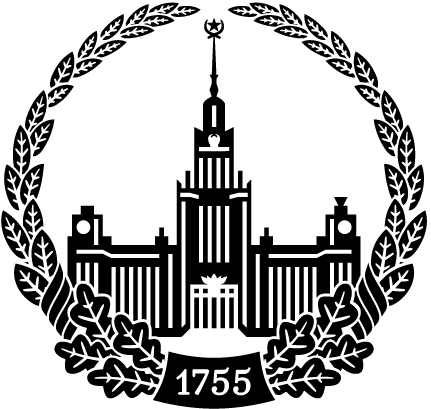
\includegraphics[width=4cm]{Logo1.png} 
		
		\vspace{1.5\baselineskip}
		\textbf{\MakeUppercase{Выпускная квалификационная работа}}
		
		\vspace{\baselineskip}
		на тему: \textbf{«Сравнение явных и неявных разностных схем для уравнения переноса»}
	\end{center}
	
	\vspace{2\baselineskip}
	
	\hfill
	\begin{minipage}{0.6\textwidth}
		\justifying
		\setlength{\parindent}{0pt}
		\hyphenpenalty=10000          % запрещаем переносы
		\exhyphenpenalty=10000
		
		\textbf{Выполнил:}\par
		студент 4 курса естественно-научного факультета направления подготовки 01.03.02~Прикладная математика и информатика\par
		{Хайбулоев Дамир\,Ахлидинович}\par
		
		\vspace{\baselineskip}
		
		\textbf{Научный руководитель:}\par
		доктор физико-математических наук, профессор кафедры вычислительной математики МГУ имени М.\,В.\,Ломоносова\par
		{Кобельков Георгий Михайлович}
		
	\end{minipage}
		
	\vfill
	
	\begin{center}
		Душанбе – 2026
	\end{center}
\end{titlepage}

\clearpage
\setcounter{page}{2}

\tableofcontents
\thispagestyle{plain}
\newpage


% ===============================
% ВВЕДЕНИЕ
% ===============================
\chapter*{ВВЕДЕНИЕ}
\addcontentsline{toc}{chapter}{ВВЕДЕНИЕ}
Уравнение переноса описывает процесс перемещения некоторой величины
в пространстве с течением времени. Это может быть концентрация вещества,
температура, плотность или любой другой скаляр, который переносится
потоком.

Ключевая особенность данного уравнения заключается в том, что сама
величина никуда не исчезает и ниоткуда не возникает, а лишь перемещается.
Если рассматривать движение отдельной частицы, то значение функции,
определённой для этой частицы, остаётся постоянным; с течением времени
изменяется только её положение в пространстве.

Отсюда следует, что решение уравнения переноса можно интерпретировать
как движение начального профиля без изменения его формы (в идеальном
случае).

% ===============================
% ПОСТАНОВКА ЗАДАЧИ
% ===============================
\section*{{Постановка задачи и физическая интерпритация}}
Рассматривается одномерное уравнение переноса вида
\begin{equation}
\frac{\partial u}{\partial t}
+ a(x,t)\frac{\partial u}{\partial x} = 0,
\label{eq:transport}
\end{equation}
где
\begin{itemize}
\item $u(x,t)$ — переносимая величина;
\item $a(x,t)$ — скорость переноса.
\end{itemize}
Задача дополняется начальными условиями
\begin{equation}
u(x,0) = u_0(x).
\label{eq:start}
\end{equation}

В работе рассматриваются следующие случаи для скорости переноса $a(x,t)$. В зависимости от вида этого коэффициента изменяется физическая картина процесса


\section*{Случай постоянной скорости $(a = const)$}


При постоянном коэффиценте весь профиль движется равномерно. Каждый элемент
системы смещается на одно и то же расстояние за одинаковые промежутки
времени. Этот случай является базовым и часто используется в качестве
эталонного при сравнении численных методов.

\section*{Скорость, зависящая от координаты $(a = a(x))$}

Если коэффициент зависит от координаты, то разные участки профиля движутся с различными
скоростями. В результате профиль может сжиматься или растягиваться.
В данном случае особенно важно, насколько корректно численная схема
передаёт изменение формы решения.

\section*{Скорость, зависящая от времени $(a = a(t))$}

Если коэффициент зависит только от времени, то весь профиль движется синхронно, однако скорость его перемещения изменяется со временм. Такой перенос называется нестационарным по времени. Форма профиля сохраняется, но расстояние, пройденное элементами системы за единицу времени, меняется, что накладывает дополнительные требования на устойчивость и точность численных методов

\section*{Нестационарная скорость}

В случае
\begin{equation}
a(x,t) = x - t
\end{equation}
процесс переноса становится нестационарным. Скорость изменяется как по
пространству, так и по времени, что приводит к более сложной динамике
решения и повышенным требованиям к устойчивости и точности численных
методов.

\section*{Основные методы решения уравнения переноса}

Все численнные методы тестируются на ступенчатых начальных условиях, так как на них можно четко рассмотреть ошибки этих методов. Так же при необходимости используют граничные условия, хотя они уменьшают количество всевозможных существующих решений. Понимание физического смысла коэффициента переноса, для определенного случая, позволяет описать поведение решения. Для получения результатов решения уравнения переноса, как ранее уже уточнялось, применятся различные аналитические и численные методы.

Аналитические методы позволяют получить точное описание решения уравнения, данные методы в основном применяются в теоретическом анализе. Однако на практике, в большинстве случаев, особенно при переменном коэффициенте переноса или сложных начальных, граничных условиях, аналитическое решение либо отсутствует, либо процесс нахождения или само решение является неудобным для использования. В таких случаях используют численные методы \cite{bakhvalov, hakimzyanov}.

\section*{Метод характеристик}

Суть метода характеристик \cite{bakhvalov, popov, hakimzyanov} заключается в том, что уравнение переноса рассматривается не в фиксированной точке, а вдоль определенных кривых, по которым движется решение уравнения, называемых характеристиками. Эти кривые описывают движение частиц среды под влиянием уравнения переноса. Вдоль каждой характеристической линии значение функции остается неизменным. Благодаря именно данному методу можно установить, что решение уравнения переноса является переноса начального распределения вдоль траекторий, определяемых коэффициентом скорости. Вид и направление данных линий напрямую зависит от коэффициента скорости. Более сложные зависимости, определяемы для этого коэффициента, влекут за собой более сложно поведение решения уравнения переноса. Метод характеристик позволяет не только получать аналитическое решение, но и интерпретировать результаты численного моделирования. Он дает возможность заранее предугадать направление скорости переноса и так же является эталоном для оценки точности разностных схем.

\section*{Метод конечных разностей}

Метод конечных разностей \cite{bakhvalov, popov, hakimzyanov} является одним из наиболее распространенных численных методов для решения уравнения переноса. Его идея заключается в замене непрерывной области определения задачи на дискретную сетку по пространству и по времени, определяемой следующим образом, вводится равномерная сетка:
\begin{gather*}
x_m = m h, \quad t^n = n \tau \\
u_m^n \approx u(x_m, t^n)
\end{gather*}
Производные, включающиеся в уравнение, аппроксимируются конечными разностями, связывающими значение решения в соседних узлах сетки. По итогу исходная дифференциальная задача сводится к системе алгебраических уравнений, позволяющих пошагово вычислить приближенное решение.

\section*{Метод неопределенных коэффициентов}

В методе неопределенных коэффициентов \cite{bakhvalov, popov, hakimzyanov} аппроксимация производных реализуется в общем виде с неизвестными коэффициентами, которые в последствие подбираются так, чтобы схема обладала заданным порядком точности. Использование данного метода дает возможность систематически создавать различные вариации явных и неявных схем, а так анализировать воздействия выбора коэффициентов на устойчивость и точность численного решения.

\section*{Интерполяционно-характеристический метод (метод обратной характеристики)}

Интерполяционно-характеристический метод \cite{bakhvalov, hakimzyanov} занимает особое место при решении уравнения переноса. Он основан на сочетании идей метода прямой характеристики и численного интерполирования. Суть метода заключается в том, что значение решения в узле сетки на новом временном слое, определяется путем переноса информации вдоль характеристики назад во времени. В основном точка начала характеристики не совпадает с узлом сетки, значение решения восстанавливается с помощью интерполяции. Данный метод позволяет сокращать численную диффузию и более точно воспроизводить процесс переноса по сравнению с классическими разностными схемами, особенно полезно при наличии резких фронтов в начальных условиях.

\section*{Явные разностные схемы}

В явных разностных \cite{bakhvalov, popov, hakimzyanov} схемах значения решения на новом временном слое вычисляется непосредственно через значение на предыдущем слое. Это делает процесс нахождения решения более простым и удобным для реализации. Явные схемы хорошо отражают физический смысл переноса, однако они требуют строгого согласования шагов сетки по времени и по пространству, в основном берут мелкие шаги по пространству, что вынуждает брать, так же мелкие шаги по времени, благодаря этому и обеспечивается устойчивость.
 
Решение устойчиво только при выполнении условия Куранта:
\begin{equation}
|\lambda| \le 1,
\end{equation}
где
\begin{equation}
|\lambda| = \frac{a\tau}{h}.
\label{number:CFL}
\end{equation}

При нарушении условия устойчивости, то есть при увеличении шага сетки по пространству, происходит взрыв решения, что ограничивает область применения таких схем, так же при малых шагах сетки значительно увеличиваются затраты времени при вычислении решения на ЭВМ.

\section*{Неявные разностные схемы}

В неявных разностных схемах \cite{bakhvalov, popov, hakimzyanov} значение решения на новом временном слое определяется из системы алгебраических уравнений, связывающей все узлы сетки между собой. Это повышает устойчивость численного решения и позволяет использовать более крупные шаги по времени. Однако, неявные схемы могут вносить дополнительное сглаживание решения, что может приводить к размыванию фронта переноса. Так же на каждом временном слое приходиться решать систему уравнений. Таким образом, повышение устойчивости достигается ценой потери точности в передаче формы решения, а также увеличения количества операций вычисления от слоя к слою.

\textit{Таким образом, исходя из всего вышесказанного, можно заключить, что решение уравнения переноса – это модельная задача, которая демонстрирует связь между физическим смыслом коэффициента переноса, аналитическим описанием и его численной реализацией. Вид коэффициента переноса $a(x, t)$ определяет характер движения решения и структуру характеристик, определяемых решением уравнения, что существенно влияет на поведение численных схем.}

\textit{Аналитический подход, реализуемый при помощи метода характеристик, позволяет получить общее представление о свойствах решения для дальнейшего анализа численного метода.}

\textit{В работе рассматриваются точность, устойчивость, диссипативные и дисперсионные свойства \cite{goloviznin}, монотонность и численная диффузия разностных методов при решении уравнения переноса для трех видов коэффициента переноса. Анализ проводиться при ступенчатых начальных условиях, что позволяет наглядно выявить особенности поведения численного решения и различия между используемыми схемами.}\\

\chapter{АНАЛИТИЧЕСКОЕ РЕШЕНИЕ}

В большинстве задач переноса и дифференциальных уравнений в общем и целом аналитическое решение найти сложно или вообще невозможно. Именно по этой причине и применяются численные методы. Они позволяют приблеженно построить решение, когда нет явной формулы.

В данной работе ситуация немного иная: для выборанных случаев коэффициента переноса    $ a(x,t)$ аналитическое решение сществует. Это дает уникальную возможность использовать данное решение как математический эталон, относительно которого можно оценить критерии численных методов, описанных в введении, таких как точность, устойчивость, диссипативные и дисперсионные свойства, монотонность и численная диффузия.

Другими словами, основная цель - не просто получить численное решение, а исследовать поведение решения при использовании численных методов, то есть насколько хорошо разностные схемы воспроизводят физический смысл процесса переноса, когда форма профиля движется, деформируется или колеблется в зависимости от типа коэффициента $a$. Так же необходимо отметить, что точность аппроксимации оценивается через физическую интерпретацию решения: сжатие, растяжение, колебания, сдвиг всего профиля и т.д.

\sectionc{Общая формула аналитического решения}

Для аналитического решения рассматривают функцию $u(x,t)$ вдоль характеристической линии $x=x(t)$. Если взять полную производную по времени от функции $u(x,t)$
\begin{equation}
\frac{du}{dt} = \frac{\partial u}{\partial t} + \frac{\partial u}{\partial x}\frac{dx}{dt}.
\end{equation}
Сравнивая данное равенство с формулой \eqref{eq:transport}, следует что если выбрать траекторию так, чтобы выполнялось
\begin{equation}
\frac{dx}{dt} = a(x,t)
\end{equation}
то производная $du/dt$ вдоль этой характеристики обращается в ноль.

Это означает, что значение функции $u$ не изменяется вдоль характеристики, а его значение в любой точке и моменте времени определяется начальными условиями \eqref{eq:start}, где при $x=x_0$ - координата начала характеристики при $t=0$, а $u_0(x)$ начальное распределение функции.

Таким образом, общее аналитическое решения уравнения переноса с переменным коэффициентом $a(x,t)$ выражается через характеристические линии \cite{bakhvalov, popov}: сначала находят траектории, затем используется начальные условия для вычисления $u$ в любой точке.

\sectionc{{Случай постоянной скорости $(a=const)$}}

В случае постоянного коэффициента переноса $a=const$ характеристические линии представляют собой прямые линии в пространственно-временной плоскости, поскольку скорость движения каждого элемента профиля одинакова

Аналитическое решения для этого случая выглядит следующим образом:
\begin{equation}
u(x,t) = \phi(x-at),
\end{equation}
где $\phi$ - функция, определяемая начальным распределнием $u_0(x)$. Это форма отражает сдвиг всего профиля вдоль оси $x$ с постоянной скоростью $a$, без изменения его формы \cite{bakhvalov, popov, sorokin, hakimzyanov}.

Для наглядного представления решения можно использовать графики в двумерной и трехмерной формах:

\begin{figure}[H]
    % Первый подрисунок
    \vspace{10pt}
    \begin{subfigure}[b]{0.45\textwidth}
        \centering
        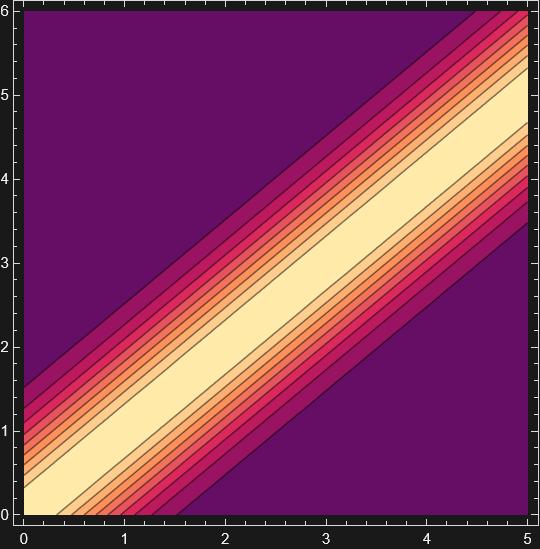
\includegraphics[width=\textwidth,height=7cm]{a_const_countur.jpg} % путь к первой картинке
        \caption{Контурный график}
        \label{fig:graph1}
    \end{subfigure}
    \hfill
    % Второй подрисунок
    \begin{subfigure}[b]{0.45\textwidth}
        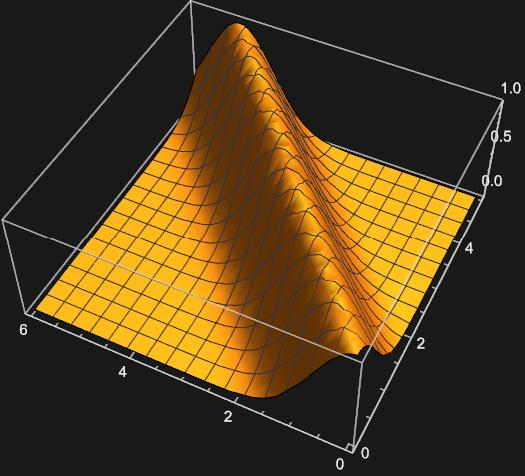
\includegraphics[width=\textwidth,height=7cm]{a_const_3d.jpg} % путь ко второй картинке
        \caption{Объёмный график}
        \label{fig:graph2}
    \end{subfigure}

    % Общая подпись для всей фигуры (если нужна)
    \caption{Характеристическое решение уравнения переноса для случая $a=const$}
    \label{fig:graphs}
\end{figure}


\sectionc{{Случая зависимости от координаты $(a = a(x))$}}

В данном случае коэффициент переноса зависит только от пространственной перенной. Из этого следует, что разные участки профиля могут двигаться с разной скоростью, даже в один и тот же момент времени. Вид изменения профиля зависит от вида коэффициента $a=a(x)$, например, профиль может растягиваться или сжиматься. Это говорит о том что перенос при данном коэфициенте является не равномерным.

Аналитическое решение будет иметь следующий вид:
\begin{equation}
u(x,t)=\phi\!\left(
\int_{1}^{x}\frac{d\theta}{a(\theta)}-t
\right)
\end{equation}

Как видно из данного равенства аналитическое решение зависит от интегрирования $1/a(x)$, получается чем сложнее будет функция $a(x)$, тем сложнее будет найти явное решение уравнения переноса при таком коэффициенте \cite{sorokin}, поэтому для дальнейшего исследования целесообразно выбирать такие функции коэффициента переноса, которые допускают явное или легкое вычисление аналитического решения.

В представленной работе будет фигурировать следующая функция коэффициента переноса:
\begin{equation}
a(x) = 1 + \frac{1}{2}\sin(x).
\end{equation}
Выбор такой функции обусловлен несколькими причинами, а именно, во-первых, она является гладкой и периодической, что соответствует физически реалистичной модели неоднородного переноса, во-вторых, при таком виде коэффициента уравнение переноса для характеристики допускает аналитическое интегрирование, вследствие чего можно явно выразить функцию $u(x,t)$.

\begin{figure}[H]
	% Первый подрисунок
	\vspace{10pt}
	\begin{subfigure}[b]{0.45\textwidth}
		\centering
		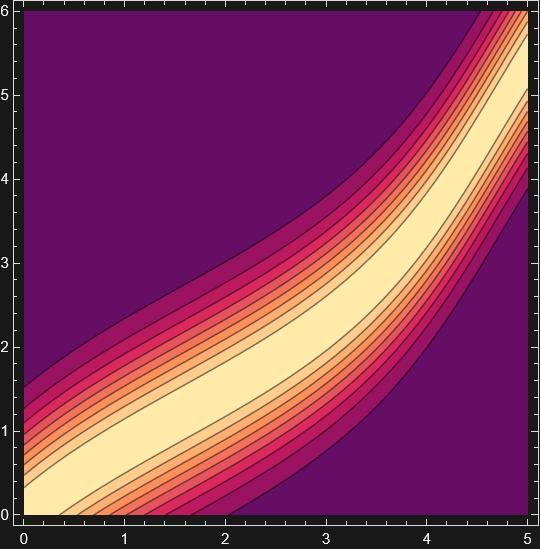
\includegraphics[width=\textwidth,height=7cm]{a_x_countur.jpg} % путь к первой картинке
		\caption{Контурный график}
		\label{fig:graph1_a_x}
	\end{subfigure}
	\hfill
	% Второй подрисунок
	\begin{subfigure}[b]{0.45\textwidth}
		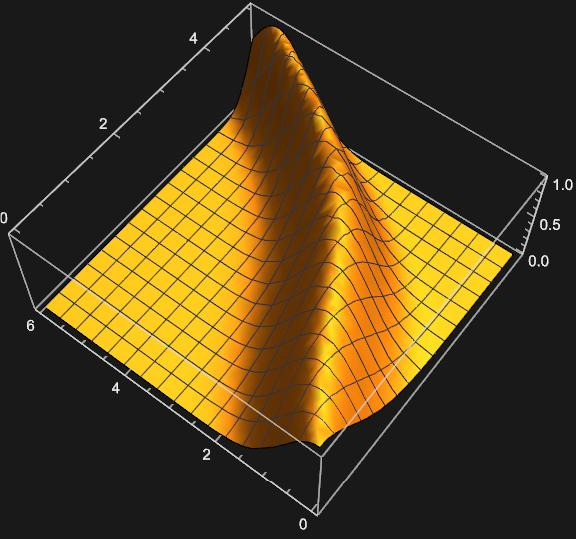
\includegraphics[width=\textwidth,height=7cm]{a_x_3d.jpg} % путь ко второй картинке
		\caption{Объёмный график}
		\label{fig:graph2_a_x}
	\end{subfigure}
	
	% Общая подпись для всей фигуры (если нужна)
	\caption{Характеристическое решение уравнения переноса для случая $a=a(x)$}
	\label{fig:graphs1}
\end{figure}

Так же важно продемонстрировать решение уравнения переноса при данном коэффициенте по характеристикам:
\begin{itemize}
	\item На контураном графике, рисунок \eqref{fig:graph1_a_x}, видно как профиль переносится и одновременно деформируется вдоль координаты $x$ в зависимости от локального значения скорости $a(x)$.
	\item На Объёмном графике, рисунок \eqref{fig:graph2_a_x}, же видно как профиль растягивается и сжимается при переносе в пространственно-временной области, что особенно важно для анализа точности численных схем.
\end{itemize}

\sectionc{{Случая зависимости от времени $(a = a(t))$}}

При таком представлении коэффициента переноса, уравнение будет зависеть только от временной пременны. Это означает что в определенный момент времени, весь профиль будет двигаться с одной и той же скоростью, однако эта скорость может меняться во времени. В отличие от предыдущего случая, здесь не возникают локальные деформации профиля относительно пространственной координаты, так как все точки профиля движутся синхронно.

Аналатическое решение для случая, зависящего от времени, выглядит следующим образом:
\begin{equation}
u(x,t)=\phi\!\left(
x -\int_{0}^{t}a(\theta)d\theta
\right)
\end{equation}

Из этого аналитического решения вытекает то что сдвиг начального профиля определяется интегралом от функции скорости $a=a(t)$.

Для дальнейшего исследования в работе будет использоваться функиция:
\begin{equation}
a(t) = (-1)^{\lfloor t \rfloor}
\end{equation}

Выбор этой функции обеспечивает периодические колебания скорости. На каждом временном интервале длины единица скорость принимает постоянное значение, последовательно меняя знак, в следствие этого профиль по очереди движется то вперед, то назад, что приводит к колебательному характеру переноса. 
\begin{figure}[H]
	\vspace{10pt}
    % Первый подрисунок
    \begin{subfigure}[b]{0.45\textwidth}
        \centering
        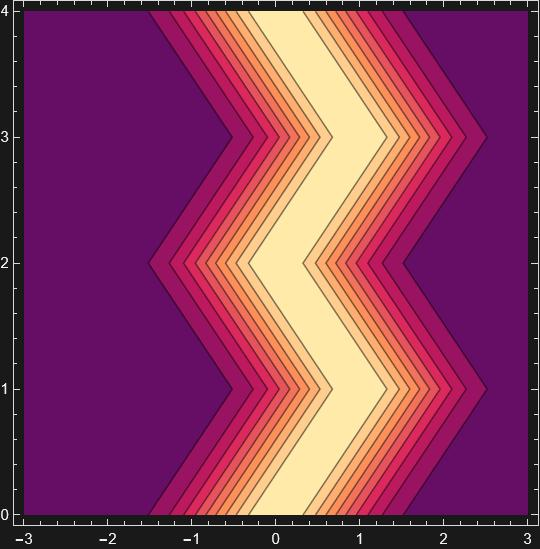
\includegraphics[width=\textwidth,height=7cm]{a_t_countur.jpg} % путь к первой картинке
        \caption{Контурный график}
        \label{fig:graph1_a_t}
    \end{subfigure}
    \hfill
    % Второй подрисунок
    \begin{subfigure}[b]{0.45\textwidth}
        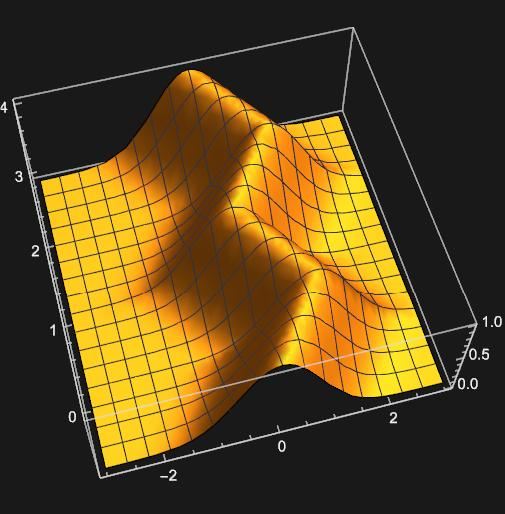
\includegraphics[width=\textwidth,height=7cm]{a_t_3d.jpg} % путь ко второй картинке
        \caption{Объёмный график}
        \label{fig:graph2_a_t}
    \end{subfigure}

    % Общая подпись для всей фигуры (если нужна)
    \caption{Характеристическое решение уравнения переноса для случая $a=a(t)$}
    \label{fig:graphs2}
\end{figure}

Данный случай представляет особый интерес при анализе численных схем, так как позволяет проверить их способность корректно воспроизводить смену направления движения.

\sectionc{{Случая нестационарной скорости $(a(x,t) = x-t)$}}

В данном случае коэффициент переноса зависит одновременно как от пространства, так и от времени. Такой тип скорости приводит к полностью нестационарному переносу, что объясняет движение и дифермацию профиля одновременно по двум этим переменным. В отличие от рассмотренных ранее случае, здесь скорость каждой точки изменяется как во времени, так и в пространстве.

Аналитика выглядит так:
\begin{equation}
u(x,t)=\phi\!\left(e^{-t}(x-t-1)\right)
\end{equation}

Полученное аналитическое решение \cite{glasner} содержит сдвиг аргумента начальной функции, в результате чего профиль в момент времени $t=0$ не проходит через начало координат. Для удобства в дальнейшем анализе выполняется эквивалентный сдвиг, позволяющий расположить профиль в нуле. Для этого можно прибавить $e^{-t}$, что даст:
\begin{equation}
u(x,t)=\phi\!\left(e^{-t}(x-t-1)+e^{-t}\right)=\phi\!\left(e^{-t}(x-t)\right)
\end{equation}

\begin{figure}[H]
	\vspace{10pt}
    % Первый подрисунок
    \begin{subfigure}[b]{0.45\textwidth}
        \centering
        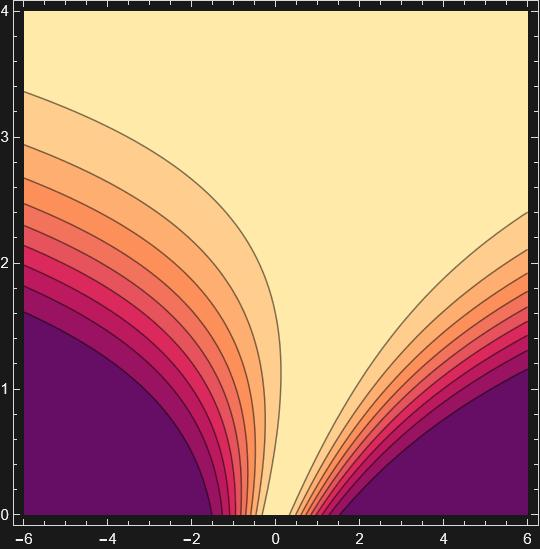
\includegraphics[width=\textwidth,height=7cm]{a_x_t_countur.jpg} % путь к первой картинке
        \caption{Контурный график}
        \label{fig:graph1_a_x_t}
    \end{subfigure}
    \hfill
    % Второй подрисунок
    \begin{subfigure}[b]{0.45\textwidth}
        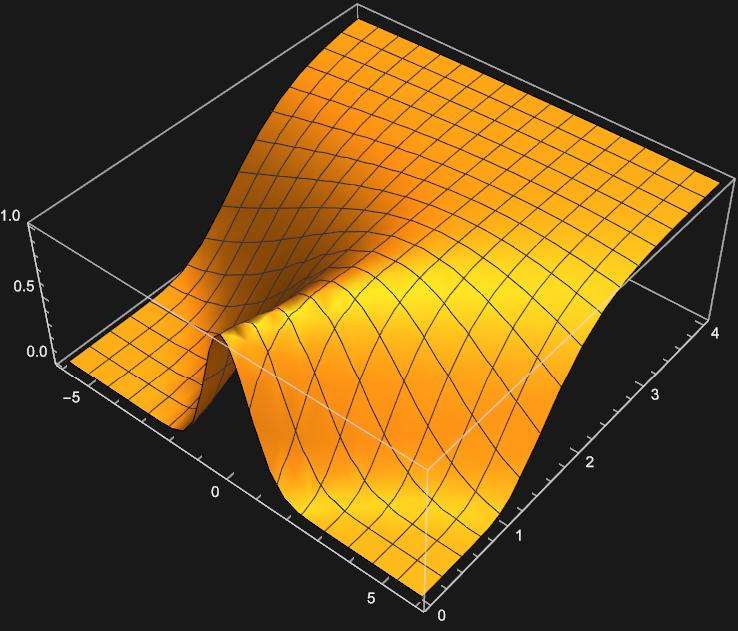
\includegraphics[width=\textwidth,height=7cm]{a_x_t_3d.jpg} % путь ко второй картинке
        \caption{Объёмный график}
        \label{fig:graph2_a_x_t}
    \end{subfigure}

    % Общая подпись для всей фигуры (если нужна)
    \caption{Характеристическое решение уравнения переноса для случая $a=x-t$}
    \label{fig:graphs3}
\end{figure}

Этот 4-ый случай является наиболее показательным для анализа численных схем, так как нестационарная скорость приводит к одновременному изменению профиля по обеим координатам. Данный аспект повышает требования к точности аппроксимации и устойчивости разностных схем. Акцент делается на возможности численных методов правильно воспроизвести сложную динамику переноса и минимизации накопления ошибок при длительных расчетах. 

\sectionc{{Итоги аналитического решения}}

В данной главе было вычисленно явное аналитическое представление для каждого из 4-ых коэффицентов переноса. Для каждого вида показано, что решение может быть получено методом характеристик и выражено через начальное условие функции.

Глава также не обошла стороной физическую интерпретацию полученных решений. В качестве примера были проиллюстрированы контурные и объёмные графики для каждого случая.
\begin{itemize}
\item Контураный график позволяет визуально оценить траектории постоянных уровней функции $u(x,t)$ и увидеть сдвиг профиля.
\item Объёмный график дает представление о рапсредлении $u(x,t)$ в пространственно --   временной области, показывая, как профиль смещается вдоль оси $x$.
\end{itemize}

Аналитические решения, полученные в этой главе будут использоваться в дальнейшем как эталон, относительно которого проводиться анализ точности, устойчивости и физической корректности разностных схем, что позволяет четко судить о качестве аппроксимации и выявлять особенности работы с тем или иным случаем коэффициента переноса.

\chapter{АППРОКСИМАЦИЯ РАЗНОСТНЫМИ СХЕМАМИ}
\sectionc{{Аппроксимация явными разностными схемами}}

В данном параграфе будет рассматриваться численная аппроксимация уравнения переноса при помощи явных разностных схем. Теоретические аспекты, а также постановка задачи были описаны во введении работы, исходя из этого основное внимание этого параграфа будет уделено практической реализации разностных схем и анализу полученных результатов.

В параграфе будут использоваться несколько различных явных разностных схем, отличающиеся различными свойствами, которые так же будут проанализированы. 

Численные эксперементы были проведены для всех видов коэффициента переноса. Такой подход позволяет проследить влияние выбора схемы на точность аппроксимации и характер численных искажений для уравнения переноса с различной сложностью коэффициента переноса.

Анализ результатов будет проводиться на основе визуального сравнения и расчета ошибки разностной аппроксимации относительно аналитического решения, что позволяет наглядно оценить качество аппроксимации и поведение явных схем при различных коэффициентах переноса.

Перед тем как дать перечень используемых явных схем, введем некоторые обозночения, посредствам которых будет легче и компактнее записывать формулы этих схем. Значение некоторой функции $u$ в узле $(m,n)$ пространственно-врменной сетки, будем обозначать через 
\[
u_m^n,
\]если индексы будут опущены, значит они равны $m$ и $n$ соответственно. Дальше, так же для сокращения, значение функции $u$ на временном слое $(n+1)$ обозначим как
\[
u_m^{n+1} = \hat{u}.
\]
Для разностных операторов применяются следующие обозначения \cite{popov}:
\begin{align}
u_t &= \frac{u_m^{\,n+1} - u_m^{\,n}}{\tau}, &
u_{\mathring{t}} &= \frac{u_m^{\,n+1} - u_m^{\,n-1}}{2\tau}, &
u_{\bar{t}} &= \frac{u_m^{\,n} - u_m^{\,n-1}}{\tau}, 
\label{form:oboz1}\\
u_x &= \frac{u_{m+1}^{\,n} - u_m^{\,n}}{h}, &
u_{\mathring{x}} &= \frac{u_{m+1}^{\,n} - u_{m-1}^{\,n}}{2h}, &
u_{\bar{x}} &= \frac{u_m^{\,n} - u_{m-1}^{\,n}}{h}.
\label{form:oboz2}
\end{align}

Теперь когда введены основные обозначения можно представить список явных разностных схем, по средствам которых проводилось исследование в данной работе.

\section*{Явная схема против потока}
\begin{equation}
u_t + a\,u_x^{\mathrm{up}} = 0,    
\end{equation}
где
\[
u_x^{\mathrm{up}} =
\begin{cases}
u_{\bar{x}} & a > 0, \\
u_x,      & a < 0.
\end{cases}
\]

\section*{Явная схема (Лакс–Фридрихс)}
\begin{equation}
    u_t
    +
    a\,u_{\mathring{x}}
    =
    \frac{1}{\tau}
    \left(
    \frac{u_{m+1}^{\,n}+u_{m-1}^{\,n}}{2}
    -
    u_m^{\,n}
    \right).
\end{equation}
откуда следует
\begin{equation*}
    \hat{u} = \frac{1}{2}\,\left(
        u_{m+1}^n + u_{m-1}^n \right) -
        a\,\frac{\tau}{2h}\,\left(
        u_{m+1}^n - u_{m-1}^n \right).
\end{equation*}

\section*{Явная схема (Лакс–Вендрофф)}
\begin{equation}
    \hat{u} = u_m^n - a\,\frac{\tau}{2h}\left(
        u_{m+1}^n-u_{m-1}^n \right)+
    a^2\,\frac{\tau^2}{2h^2}\left(
        u_{m+1}^{n} - 2\,u_m^n + u_{m-1}^n \right)
\end{equation}

\section*{Центральная явная схема с искусственной вязкостью}
\begin{equation}
    u_t + a\,u_{\mathring{x}}=\frac{h^4}{2}\,u_{\bar{x}x},
\end{equation}
где
\[
u_{\bar{x}x} =\frac{u_{m+1}^n - 2\,u_m^n + u_{m-1}^n}{h^2} 
\]
откуда получаем
\begin{equation*}
    \hat{u}=u_m^n + a\,\frac{\tau}{2h}\left(
        u_{m+1}^{n}-u_{m-1}^n \right)
    +\frac{h^2}{2}\left(
        u_{m+1}^n - 2\,u_m^n + u_{m-1}^n \right)
\end{equation*}

\section*{Явная схема Мак-Кормака}
Схема Мак-Кормака - это 2-х шаговая схема, состоящая из прогноза -- это явный шаг по прямой разности:
\begin{equation}
    u_m^* = u_m^n - a\, \frac{\tau}{h}\left(
        u_{m+1}^n-u_m^n\right)
\end{equation}
и коррекции -- это общая разность:
\begin{equation}
    \hat{u} = \frac{1}{2}\left(
        u_m^n + u_m^* - a\,  \frac{\tau}{h}\left(
            u_m^*-u_{m-1}^*\right)
        \right)
\end{equation}

\section*{Явная схема Русанова}
Основная идея схемы заключается в вычислении численных потоков на границах ячеек с использованием средних значений и диссипативного члена.
Численный поток в схеме Русанова зависит от знака скорости \(a_m\):\\
\[
f_{m+1/2} = \frac{a_{m/2}}{2} \,(u_m^n + u_{i+m}^n) - \frac{|a_{m/2}|}{2} \,(u_{m+1}^n - u_m^n),\]
\[
f_{m-1/2} = \frac{a_{m/2}}{2} \,(u_{m-1}^n + u_m^n) - \frac{|a_{m/2}|}{2} \,(u_m^n - u_{m-1}^n),
\]
Значение функции на следующем временном слое вычисляется по формуле:
\begin{equation}
    \hat{u} = u_m^n - \frac{\tau}{h}\,(f_{m+1/2} - f_{m-1/2}), 
\end{equation}

\section*{Явная схема Годунова}
Схема Годунова учитывает направление волны: численный поток на границе выбирает значение из ячейки, откуда "приходит" волна.  
Численный поток на правой границе \(m+1/2\) вычисляется как
\[
f_{m+1/2} =
\begin{cases}
a_{m+1/2}\, u_m^n, & a_{m+1/2} > 0,\\[2mm]
a_{m+1/2}\, u_{m+1}^n, & a_{m+1/2} < 0,
\end{cases}
\]
на левой границе \(m-1/2\) соответственно:
\[
f_{m-1/2} =
\begin{cases}
a_{m-1/2}\, u_{m-1}^n, & a_{m-1/2} > 0,\\[2mm]
a_{m-1/2}\, u_m^n, & a_{m-1/2} < 0.
\end{cases}
\]
Значение функции на следующем временном слое вычисляется по формуле
\begin{equation}
\hat{u} = u_m^n - \frac{\tau}{h}\,(f_{m+1/2} - f_{m-1/2}).
\end{equation}

\section*{TVD-схема}

TVD-схема (Total Variation Diminishing) \cite{popov} — это схема с ограничением вариации, которая предотвращает появление численных осцилляций вблизи разрывов и сохраняет монотонность решения.

Основная идея заключается в следующем: численный поток на границе ячейки корректируется с помощью лимитирующей функции \(\phi\), которая ограничивает перепад между соседними ячейками.Рассмотрим явную TVD-схему, учитывающую знак скорости \(a_m\).  
Для внутренней ячейки \(i\) вычисляются левые и правые разности:
\[
\Delta_- = u_i^n - u_{i-1}^n, \quad
\Delta_+ = u_{i+1}^n - u_i^n.
\]
В зависимости от направления потока (\(a_i > 0\) или \(a_i < 0\)) используются соответствующие разности для построения коэффициента градиента:
\[
r_i = \frac{\Delta_-}{\Delta_+}, \quad 
\phi_i = \max\bigl(0, \min(1, r_i)\bigr),
\]
аналогично для "левой" границы:
\[
r_{i-1} = \frac{\Delta_{\text{left}-}}{\Delta_{\text{left}+}}, \quad 
\phi_{i-1} = \max\bigl(0, \min(1, r_{i-1})\bigr).
\]
Численное обновление на следующем временном слое имеет вид:
\begin{equation}
\hat{u} = u_i^n 
- \operatorname{sign}(a_i)\,\lambda_i \,\Delta_- 
- \frac{\lambda_i (1-\lambda_i)}{2} \bigl(\phi_i \Delta_+ - \phi_{i-1} \Delta_-\bigr),
\end{equation}
где \(\lambda_i = |a_i|\tau/h\) — локальное число Куранта.

Эта схема объединяет устойчивость схемы против потока с высокоточной TVD-коррекцией, подавляя численные осцилляции около разрывов, но сохраняя точность для гладких участков.

\section*{MUSCL-схема}

MUSCL-схема (Monotonic Upstream-centered Scheme for Conservation Laws) \cite{popov} является развитием TVD-схем и обеспечивает высокий порядок аппроксимации (второй порядок) для гладких участков решения, сохраняя монотонность и подавляя численные осцилляции около разрывов.  

В отличие от стандартной TVD-схемы, MUSCL использует более гибкую функцию ограничения (лимитер), например, Superbee, которая позволяет усиливать градиенты в гладких областях и одновременно предотвращает появление новых экстремумов:
\[
\phi(r) = \max\big(0, \min(2r, 1), \min(r, 2)\big).
\]
Обновление решения на внутренней ячейке \(i\) с учётом направления скорости \(a_i\) имеет вид:
\begin{equation}
u_i^{n+1} = u_i^n 
- \operatorname{sign}(a_i)\,\lambda_i \,\Delta_- 
- \frac{\lambda_i (1-\lambda_i)}{2} \bigl(\phi_i \Delta_+ - \phi_{i-1} \Delta_-\bigr),
\end{equation}
где
\[
\Delta_- = u_i^n - u_{i-1}^n, \quad
\Delta_+ = u_{i+1}^n - u_i^n, \quad
\lambda_i = |a_i|\,\frac{\tau}{h}.
\]

Таким образом, MUSCL-схема сочетает устойчивость подхода против потока с высокой точностью второго порядка и улучшенным лимитером, что делает её более точной по сравнению с обычной TVD-схемой для гладких участков решения.

Теперь для дальнейших визуальных представлений данных схем, необходимо их определить какими-нибудь цветами, чтобы было отчетливо видно как та или иная схема аппроксимирует решение уравнения переноса.На рисунке \eqref{fig:example} будут названия и цвета схем, которые дальше будут применяться.

\begin{figure}[H]
	\vspace{10pt}
    \centering
    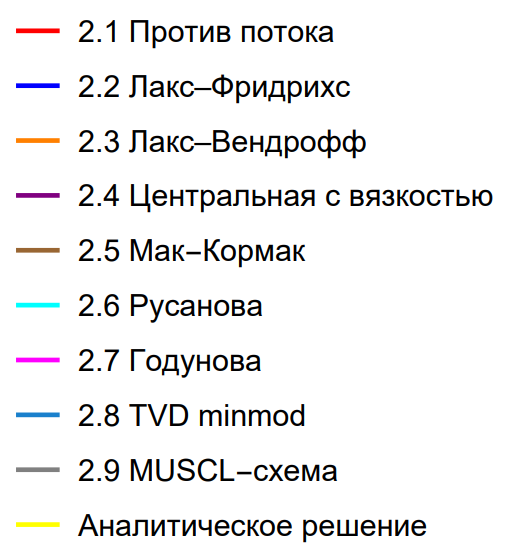
\includegraphics[width=0.45\textwidth,height=6cm,keepaspectratio]{image_2026-01-22_22-56-17.png}
    \caption{Дальнейшее обозначение явных разностных схем}
    \label{fig:example}
\end{figure}

\section*{{Случай постоянного коэффициента переноса $(a=const)$}}

Параметры аппроксимации для явных схем данного вида коэффициента переноса выглядят следующим образом:
\[
\begin{aligned}
a &= 1, \\
h &= 0.25, \\
\tau &= 0.05, \\
x &\in [-10,\,10], \\
N &= 200.
\end{aligned}
\]

Данные параметры полностью описывают пространственно -- временную сетку, так же по этим параметрам можно вычислить число Куранта по формуле \eqref{number:CFL}, применив эту формулу получим следующее значение:
 \[
 \lambda = \frac{|a|\tau}{h}=\frac{1 \cdot 0.05}{0.25} = 0.2\,<\,1
 \]
Полученное значение соответствует условию устойчивости для явных разностных схем.

Ниже будут приведены результаты численной аппроксимации вышеописанными явными схемами при постоянном коэффициенте переноса. В качестве функции для проверки явных схем  используется функция типа "ступенька". Выбор такой функции обусловлен тем, что при резких скачках численные схемы испытывают наибольшие трудности: именно при такой функции проявляются дисперсия, рассеевание и возможные осцилляции.

Визуальная состовляющая отлично отражает аппроксимацию всеми явными схемами и на рисунках это наглядно продемонстрированно. Для более объективной оценки, а не оценки на глаз, полезно рассчитать нормы ошибок явных схем относительно аналитического решения.

\begin{figure}[!ht]
	\vspace{10pt}
    \centering
    % Первая строка
    \begin{subfigure}[b]{0.45\textwidth}
        \centering
        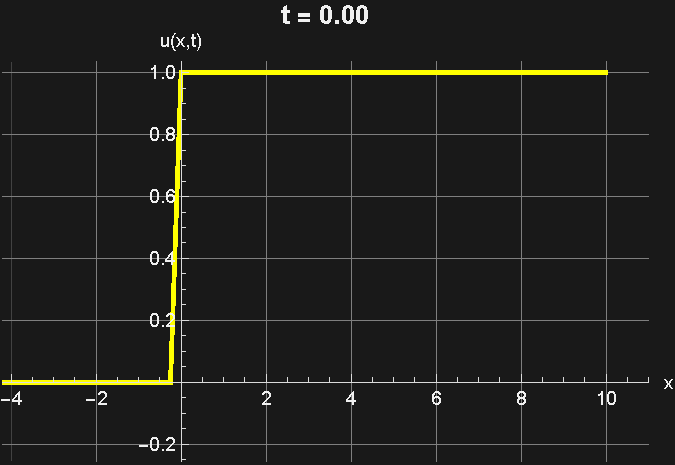
\includegraphics[height=5cm, keepaspectratio]{a_const_t_0.pdf}
        \caption{Момент времени t=0}
    \end{subfigure}
    \hspace{0.05\textwidth}
    \begin{subfigure}[b]{0.45\textwidth}
        \centering
        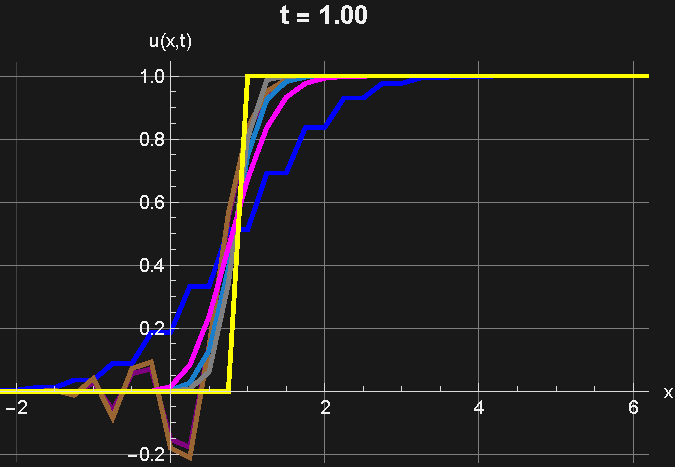
\includegraphics[height=5cm, keepaspectratio]{a_const_1.pdf}
        \caption{Момент времени t=T/10}
    \end{subfigure}

    \vspace{0.5cm}

    % Вторая строка
    \begin{subfigure}[b]{0.45\textwidth}
        \centering
        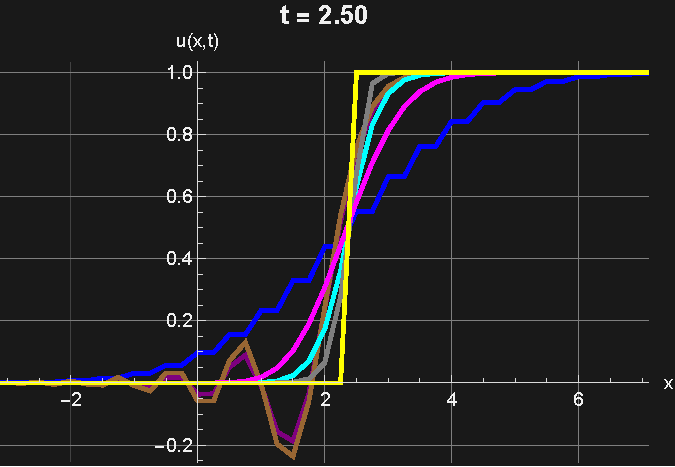
\includegraphics[height=5cm, keepaspectratio]{a_const_t_2_5.pdf}
        \caption{Момент времени t=T/4}
    \end{subfigure}
    \hspace{0.05\textwidth}
    \begin{subfigure}[b]{0.45\textwidth}
        \centering
        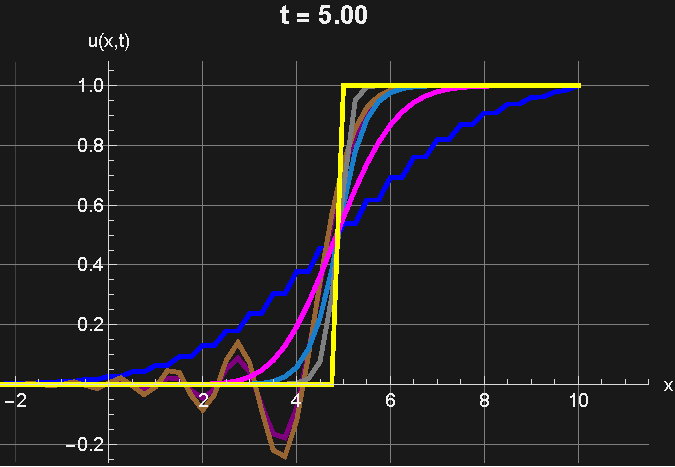
\includegraphics[height=5cm, keepaspectratio]{a_const_t_5.pdf}
        \caption{Момент времени t=T/2}
    \end{subfigure}

    \vspace{0.5cm}

    % Третья строка
    \begin{subfigure}[b]{0.45\textwidth}
        \centering
        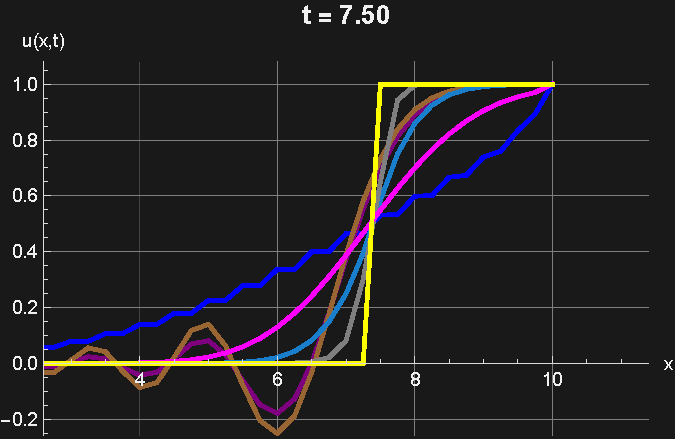
\includegraphics[height=5cm, keepaspectratio]{a_const_7_50.pdf}
        \caption{Момент времени t=3/4T}
    \end{subfigure}
    \hspace{0.05\textwidth}
    \begin{subfigure}[b]{0.45\textwidth}
        \centering
        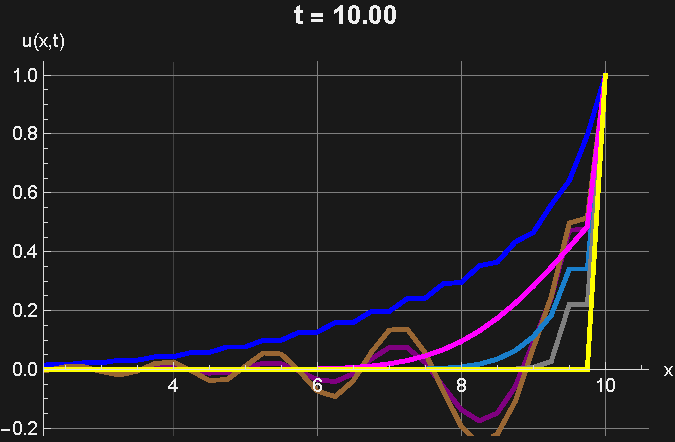
\includegraphics[height=5cm, keepaspectratio]{a_const_10.pdf}
        \caption{Момент времени t=T}
    \end{subfigure}

    \caption{Сравнение аппроксимаций для всех схем при $a=\text{const}$}
    \label{fig:all_schemes}
\end{figure}

В таблице \ref{tab:norms_compact3} приведены расчеты трех стандартных норм ошибок ($L_1$, $L_2$,$L_\infty$) для всех схем \cite{popov}. 

Средняя абсолютная ошибка ($L_1$)
\begin{equation}
	\| \text{err} \|_{L_1} = h\sum_{i} \big| u_i^{\text{num}} - u_i^{\text{exact}} \big|
\end{equation} 
показывает среднее отклонение численного решения от аналитического на всем пространстве, где определено решение. 

Среднеквадратичная ошибка ($L_2$)
\begin{equation}
		\| \text{err} \|_{L_2} = \sqrt{h\sum_{i} \big( u_i^{\text{num}} - u_i^{\text{exact}} \big)^2}
\end{equation}
учитывает квадратичное отклонение и более чувствительна к локальным ошибкам.

Максимальная ошибка ($L_\infty$) 
\begin{equation}
		\| \text{err} \|_{L_\infty} = \max_i \, \big| u_i^{\text{num}} - u_i^{\text{exact}} \big|
\end{equation}
показывает максимальное отклонение в любой точке сетки.
Тогда из таблицы \ref{tab:norms_compact3} можно сделать следующие выводы, а именно:
\begin{itemize}
	\item Малые значения $L_1$ и $L_2$ говорят о хорошей средней точности схем и малой рассеяности ошибки по всей сетке.
	\item Мало значение для нормы $L_\infty$ указывает на отсутствие крупных локальных ошибок, данный аспект важен при аппроксимации решений с резкими фронтами
\end{itemize}

Таблица \ref{tab:norms_compact3} дает возможность сравнивать решение по схемам не только по рисункам, а количественно их сопоставлять и определять, какие из них обеспечивают наименьшую ошибку в среднем и по максимуму, а так же выявить схемы с повышенной дисперсией или рассееванием численного решения.

\begin{table}[H]
\centering
\caption{Нормы ошибок для всех схем при $a=\text{const}$}
\label{tab:norms_compact3}
\small
\adjustbox{max width=\textwidth}{
\begin{tabular}{|c|c|*{10}{c|}}
\hline
\rotatebox{90}{Норма} & $t$ 
& \rotatebox{90}{Против Потока }
& \rotatebox{90}{ЛФ}
& \rotatebox{90}{ЛВ}
& \rotatebox{90}{Центр. Вязк.}
& \rotatebox{90}{Мак-Кормак}
& \rotatebox{90}{TVD}
& \rotatebox{90}{MUSCL}
& \rotatebox{90}{Русанов}
& \rotatebox{90}{Годунов} \\
\hline
\multirow{6}{*}{$L_1$}
 & 0       & 0     & 0     & 0     & 0     & 0     & 0     & 0     & 0     & 0 \\
 & $T/10$  & 0.349 & 0.863 & 0.386 & 0.355 & 0.386 & 0.224 & 0.152 & 0.349 & 0.349 \\
 & $T/4$   & 0.559 & 1.375 & 0.540 & 0.475 & 0.540 & 0.319 & 0.180 & 0.559 & 0.559 \\
 & $T/2$   & 0.792 & 1.931 & 0.726 & 0.616 & 0.726 & 0.411 & 0.198 & 0.792 & 0.792 \\
 & $3/4T$  & 0.963 & 1.987 & 0.830 & 0.682 & 0.830 & 0.476 & 0.205 & 0.963 & 0.963 \\
 & $T$     & 0.563 & 1.584 & 0.734 & 0.532 & 0.734 & 0.255 & 0.100 & 0.563 & 0.563 \\
\hline
\multirow{6}{*}{$L_2$}
 & 0       & 0     & 0     & 0     & 0     & 0     & 0     & 0     & 0     & 0 \\
 & $T/10$  & 0.317 & 0.499 & 0.314 & 0.299 & 0.314 & 0.238 & 0.192 & 0.317 & 0.317 \\
 & $T/4$   & 0.403 & 0.633 & 0.372 & 0.350 & 0.372 & 0.289 & 0.217 & 0.403 & 0.403 \\
 & $T/2$   & 0.482 & 0.759 & 0.444 & 0.412 & 0.444 & 0.332 & 0.233 & 0.482 & 0.482 \\
 & $3/4T$  & 0.533 & 0.795 & 0.458 & 0.421 & 0.458 & 0.358 & 0.236 & 0.533 & 0.533 \\
 & $T$     & 0.411 & 0.786 & 0.425 & 0.364 & 0.425 & 0.246 & 0.132 & 0.411 & 0.411 \\
\hline
\multirow{6}{*}{$L_\infty$}
 & 0       & 0     & 0     & 0     & 0     & 0     & 0     & 0     & 0     & 0 \\
 & $T/10$  & 0.317 & 0.416 & 0.493 & 0.479 & 0.493 & 0.325 & 0.283 & 0.317 & 0.317 \\
 & $T/4$   & 0.444 & 0.446 & 0.542 & 0.522 & 0.542 & 0.368 & 0.323 & 0.444 & 0.444 \\
 & $T/2$   & 0.480 & 0.505 & 0.608 & 0.582 & 0.608 & 0.423 & 0.364 & 0.480 & 0.480 \\
 & $3/4T$  & 0.467 & 0.468 & 0.582 & 0.553 & 0.582 & 0.416 & 0.350 & 0.467 & 0.467 \\
 & $T$     & 0.472 & 0.785 & 0.474 & 0.444 & 0.474 & 0.316 & 0.186 & 0.472 & 0.472 \\
\hline
\end{tabular}
}
\end{table}

Так же необходимо отметить то, что значения приведенные в таблице для некоторых схем являются одинаковыми, например, значения для схемы "Против потока", "Годунова", "Русанова". Это обусловлено тем, что схемы "Годунова" и "Русанова" являются схемами, которые аппроксимируют консервативные уравнения переноса, а при постоянном коэффициенте переноса консервативная форма $(a\,u)_x$ и неконсервативная равны $a\,u_x$, поэтому значения одинаковые.

Для большей наглядости так же будут приведены графики ошибок.
\begin{figure}[H]
	\vspace{10pt}
	\centering
	% Первая строка
	\begin{subfigure}[b]{0.45\textwidth}
		\centering
		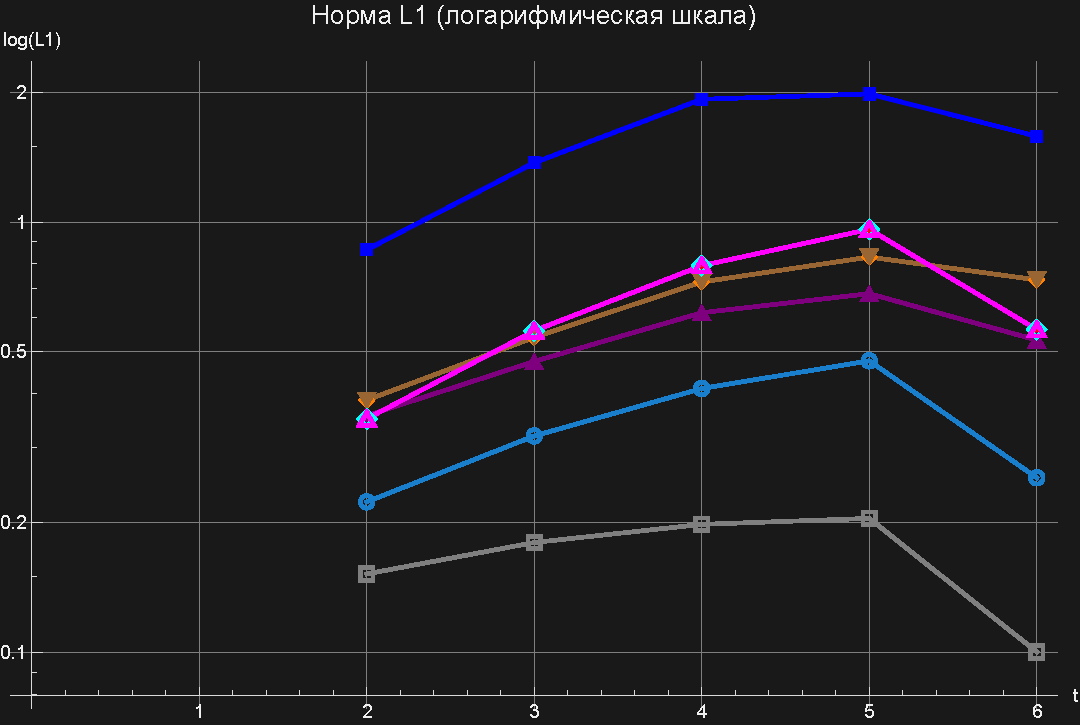
\includegraphics[height=5cm, keepaspectratio]{a_const_log_err_l1.pdf}
		\caption{Логарифмический график ошибок для нормы $L_1$}
	\end{subfigure}
	\hspace{0.05\textwidth}
	\begin{subfigure}[b]{0.45\textwidth}
		\centering
		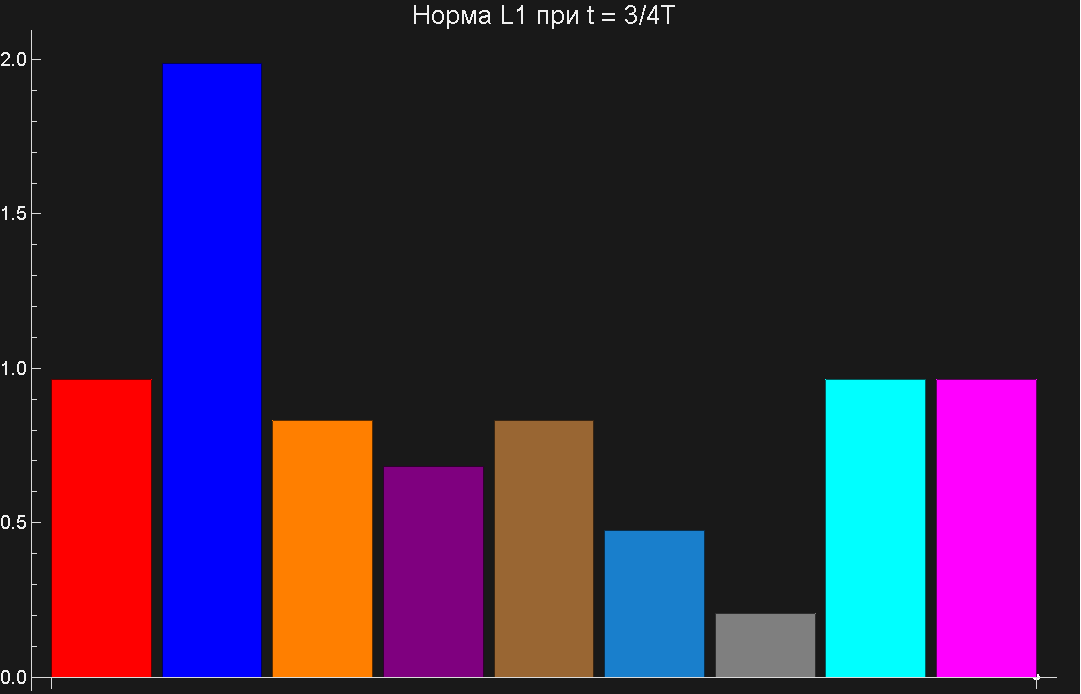
\includegraphics[height=5cm, keepaspectratio]{a_const_bar_err_l1.pdf}
		\caption{Столбчатая диаграмма ошибки для нормы $L_1$ при t=3/4T}
	\end{subfigure}
	
	\vspace{0.5cm}
	
	% Вторая строка
	\begin{subfigure}[b]{0.45\textwidth}
		\centering
		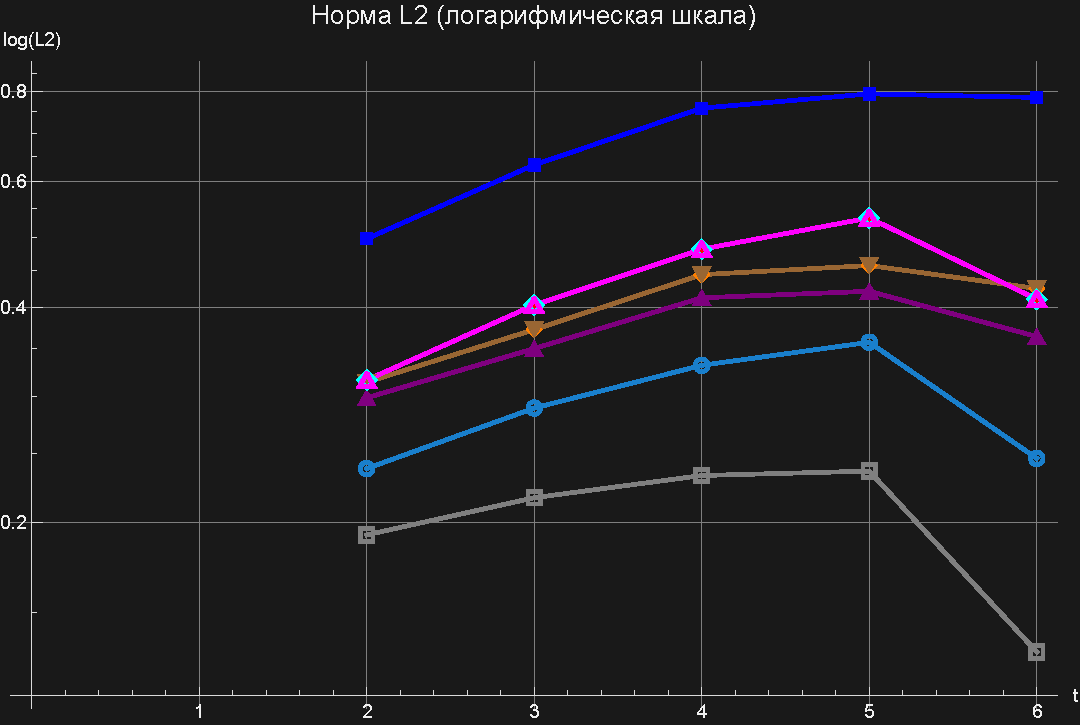
\includegraphics[height=5cm, keepaspectratio]{a_const_log_err_l2.pdf}
		\caption{Логарифмический график ошибок для нормы $L_2$}
	\end{subfigure}
	\hspace{0.05\textwidth}
	\begin{subfigure}[b]{0.45\textwidth}
		\centering
		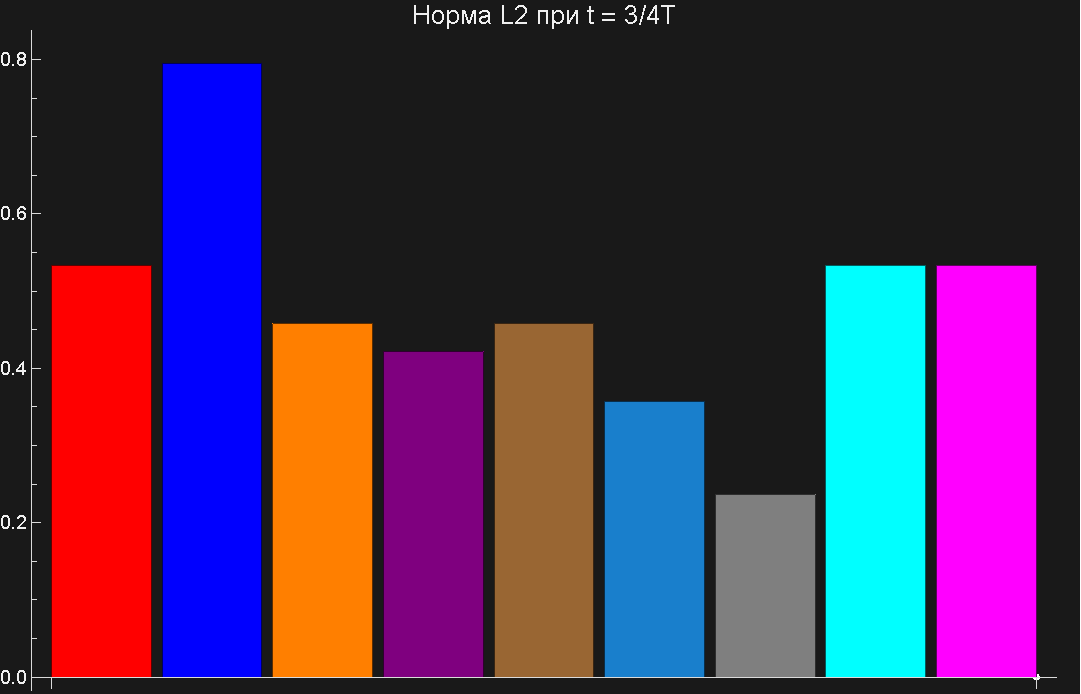
\includegraphics[height=5cm, keepaspectratio]{a_const_bar_err_l2.pdf}
		\caption{Столбчатая диаграмма ошибки для нормы $L_2$ при t=3/4T}
	\end{subfigure}
	
	\vspace{0.5cm}
	
	% Третья строка
	\begin{subfigure}[b]{0.45\textwidth}
		\centering
		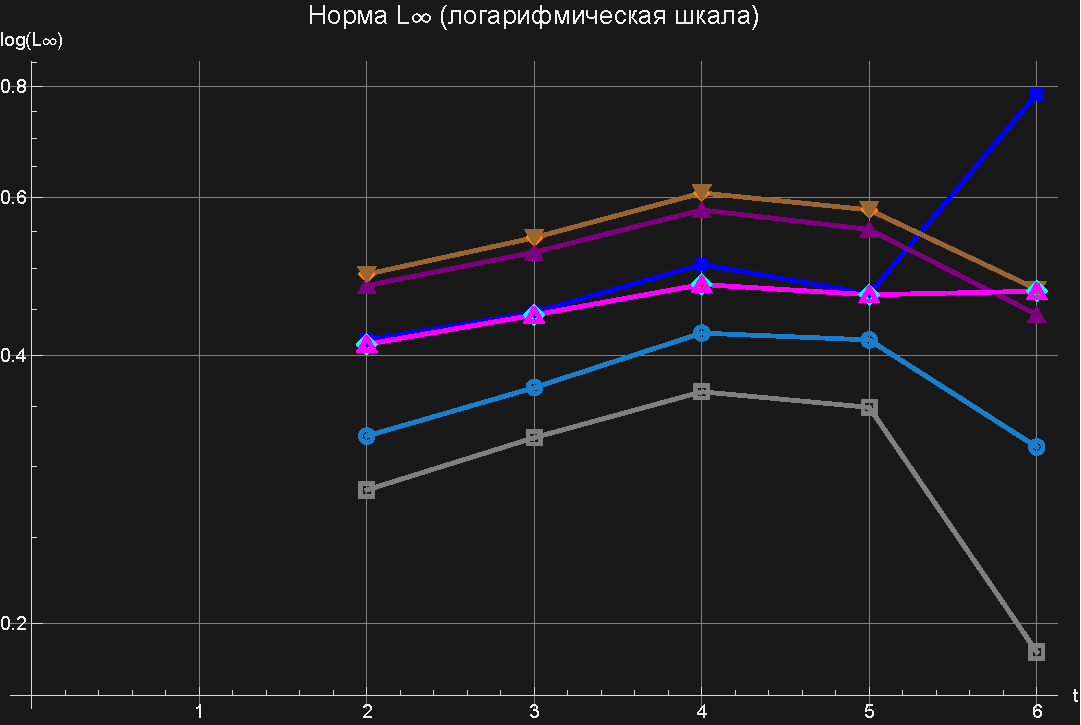
\includegraphics[height=5cm, keepaspectratio]{a_const_log_err_linf.pdf}
		\caption{Логарифмический график ошибок для нормы $L_\infty$}
	\end{subfigure}
	\hspace{0.05\textwidth}
	\begin{subfigure}[b]{0.45\textwidth}
		\centering
		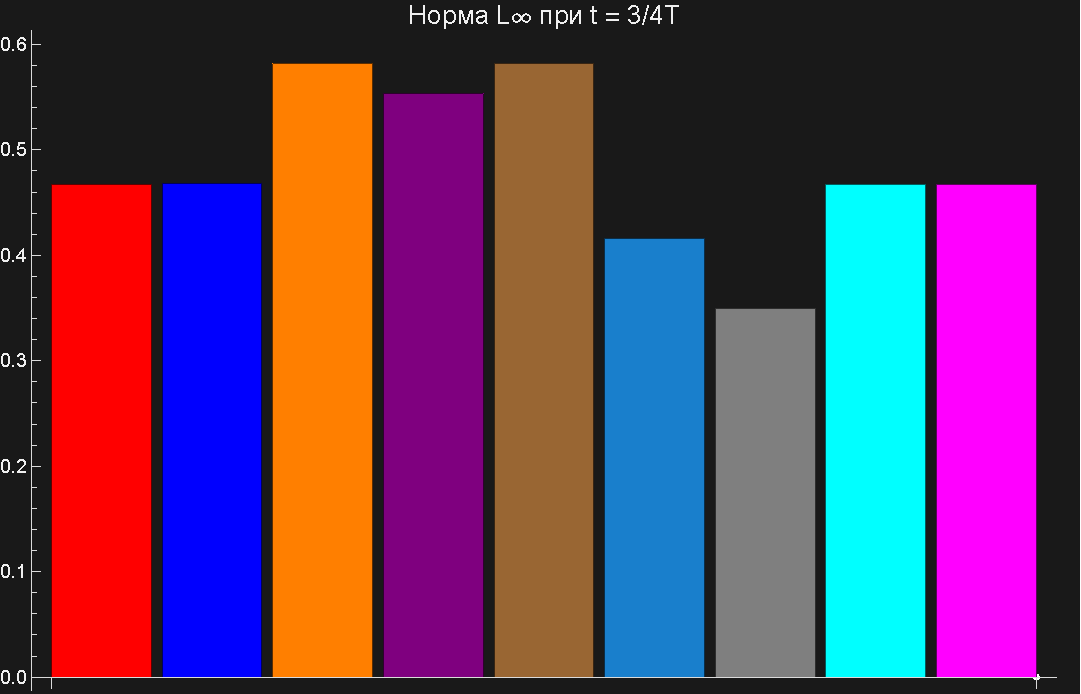
\includegraphics[height=5cm, keepaspectratio]{a_const_bar_err_linf.pdf}
		\caption{Столбчатая диаграмма ошибки для нормы $L_\infty$ при t=3/4T}
	\end{subfigure}
	
	\caption{Сравнение ошибок норм при $a=\text{const}$}
	\label{fig:all_schemes_err}
\end{figure}
На логарифмических графиках, изображенных в первом столбце, цифрами обозначены моменты времени, соответствующие данным в таблице \ref{tab:norms_compact3}.


\section*{{Случай коэффициента, зависящего от пространства $(a=a(x))$}}

Параметры аппроксимации для случая коэффициента, зависящего от пространства:
\[
\begin{aligned}
	a(x) &= 1\,+\,\frac{1}{2}\,\sin(x). \\
	h &= 0.25, \\
	\tau &= 0.05, \\
	x &\in [-20,\,20], \\
	N &= 500.
\end{aligned}
\]

Как ранее отмечалось данный случай характеризуется неравномерным переносом, отсюда следует что перенос при пространственно-зависящем коэффициенте, определяется локальными значениями скорости в каждой точке.

Визуальная составляющая приведенная на рисунке \ref{fig:all_schemes_a_x} демонстрирует неравномерный перенос профиля, локальные деформации профиля и изменение формы ступенчатой функции.

Из таблицы \ref{tab:norms_compact4} видна та же ситуация, что в прошлом случае, а именно, для трех схем "против потока", "Русанова", "Годунова" численная аппроксимация дает одинаковые значения, это обусловлено тем, что уравнение переноса, которое аппроксимируется является неконсервативным. В общем случае при пространственно коэффициенте $a=a(x)$ уравнение вида:
\begin{equation*}
	u_t\,+\,a(x)\,u_x=0
\end{equation*}
не является консервативным и не может быть приведено к дивергентной форме без добавления дополнительных членов. Схемы Годунова и Русанова, являясь методами для решения законов сохранения, применимы только для уравнений, записанных в консервативной форме, например:
\begin{equation*}
	u_t\,+\,(a(x)\,u)_x=0
\end{equation*}

\begin{figure}[H]
	\vspace{10pt}
	\centering
	% Первая строка
	\begin{subfigure}[b]{0.45\textwidth}
		\centering
		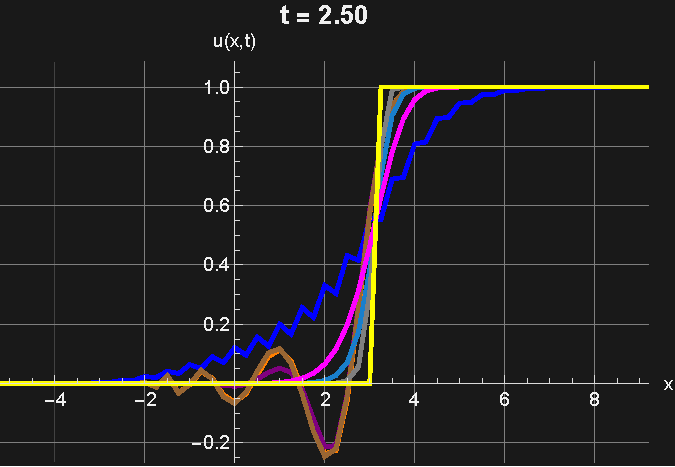
\includegraphics[height=5cm, keepaspectratio]{a_x_t_2_5.pdf}
		\caption{Момент времени t=2.5}
	\end{subfigure}
	\hspace{0.05\textwidth}
	\begin{subfigure}[b]{0.45\textwidth}
		\centering
		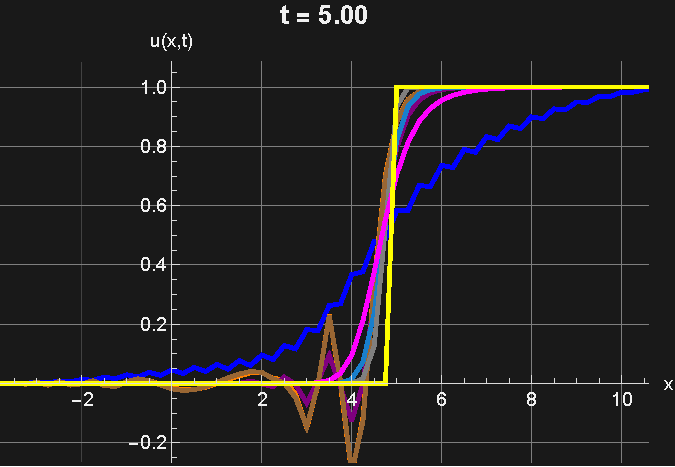
\includegraphics[height=5cm, keepaspectratio]{a_x_t_5.pdf}
		\caption{Момент времени t=5}
	\end{subfigure}
	
	\vspace{0.5cm}
	
	% Вторая строка
	\begin{subfigure}[b]{0.45\textwidth}
		\centering
		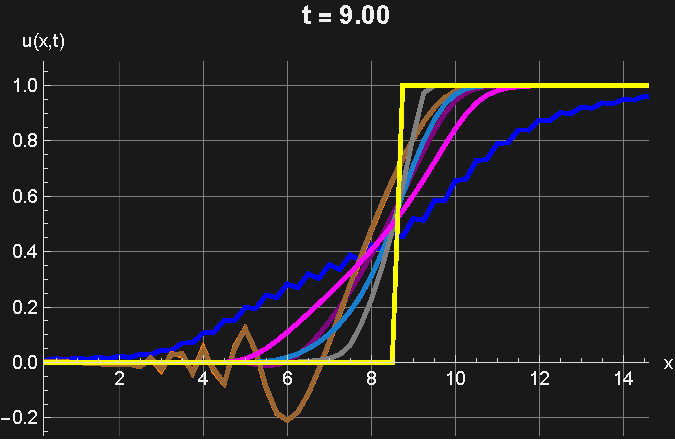
\includegraphics[height=5cm, keepaspectratio]{a_x_t_9.pdf}
		\caption{Момент времени t=9}
	\end{subfigure}
	\hspace{0.05\textwidth}
	\begin{subfigure}[b]{0.45\textwidth}
		\centering
		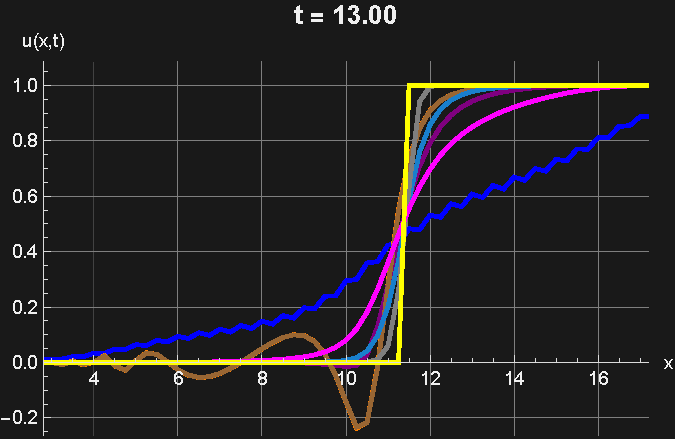
\includegraphics[height=5cm, keepaspectratio]{a_x_t_13.pdf}
		\caption{Момент времени t=13}
	\end{subfigure}
	
	\vspace{0.5cm}
	
	% Третья строка
	\begin{subfigure}[b]{0.45\textwidth}
		\centering
		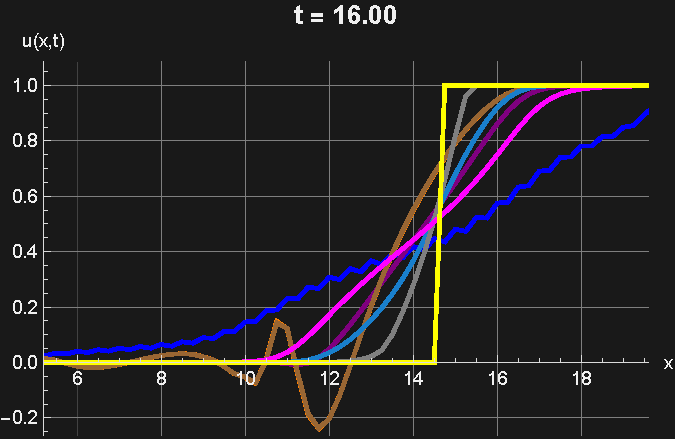
\includegraphics[height=5cm, keepaspectratio]{a_x_t_16.pdf}
		\caption{Момент времени t=16}
	\end{subfigure}
	\hspace{0.05\textwidth}
	\begin{subfigure}[b]{0.45\textwidth}
		\centering
		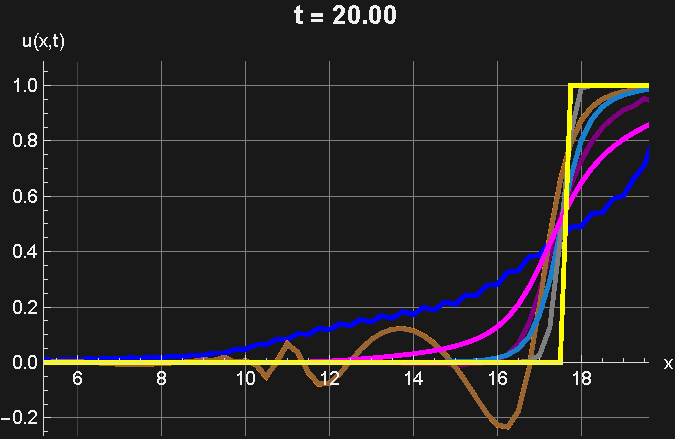
\includegraphics[height=5cm, keepaspectratio]{a_x_t_20.pdf}
		\caption{Момент времени t=20}
	\end{subfigure}
	
	\caption{Сравнение аппроксимаций для всех схем при $a=a(x)$}
	\label{fig:all_schemes_a_x}
\end{figure}
В связи с этим для численного решения данные схемы превращаются в схему "Против потока", аппроксимирующая член $a(x)\,u_x$, и учитывающая локальное напрвления переноса. Если аппроксимировать неконсервативную форму уравнения переноса схемами Годунова и Русанова, будут иметься колебания не только около разрыва, но и на всем интервале, где определена начальная функция.\\

\begin{table}[H]
	\centering
	\caption{Нормы ошибок для всех схем при $a=a(x)$}
	\label{tab:norms_compact4}
	\small
	\adjustbox{max width=\textwidth}{
		\begin{tabular}{|c|c|*{10}{c|}}
			\hline
			\rotatebox{90}{Норма} & $t$
			& \rotatebox{90}{Против Потока }
			& \rotatebox{90}{ЛФ}
			& \rotatebox{90}{ЛВ}
			& \rotatebox{90}{Центр. Вязк.}
			& \rotatebox{90}{Мак-Кормак}
			& \rotatebox{90}{TVD}
			& \rotatebox{90}{MUSCL}
			& \rotatebox{90}{Русанов}
			& \rotatebox{90}{Годунов} \\
			\hline
			\multirow{6}{*}{$L_1$}
			& 2.5  & 0.495 & 1.414 & 0.586 & 0.474 & 0.606 & 0.273 & 0.147 & 0.495 & 0.495 \\
			& 5    & 0.519 & 1.833 & 0.593 & 0.408 & 0.597 & 0.290 & 0.186 & 0.519 & 0.519 \\
			& 9    & 1.367 & 2.798 & 1.187 & 0.957 & 1.188 & 0.795 & 0.467 & 1.367 & 1.367 \\
			& 13   & 1.068 & 3.292 & 0.780 & 0.596 & 0.774 & 0.443 & 0.190 & 1.068 & 1.068 \\
			& 16   & 1.746 & 3.384 & 1.463 & 1.266 & 1.460 & 0.998 & 0.529 & 1.746 & 1.746 \\
			& 20   & 1.209 & 2.541 & 1.054 & 0.707 & 1.047 & 0.506 & 0.192 & 1.209 & 1.209 \\
			\hline
			\multirow{6}{*}{$L_2$}
			& 2.5  & 0.378 & 0.638 & 0.385 & 0.377 & 0.393 & 0.265 & 0.187 & 0.378 & 0.378 \\
			& 5    & 0.403 & 0.702 & 0.453 & 0.363 & 0.447 & 0.316 & 0.275 & 0.403 & 0.403 \\
			& 9    & 0.662 & 0.925 & 0.618 & 0.555 & 0.623 & 0.482 & 0.381 & 0.662 & 0.662 \\
			& 13   & 0.528 & 0.999 & 0.412 & 0.399 & 0.407 & 0.335 & 0.229 & 0.528 & 0.528 \\
			& 16   & 0.766 & 1.053 & 0.712 & 0.653 & 0.715 & 0.553 & 0.416 & 0.766 & 0.766 \\
			& 20   & 0.584 & 0.885 & 0.503 & 0.448 & 0.498 & 0.359 & 0.236 & 0.584 & 0.584 \\
			\hline
			\multirow{6}{*}{$L_\infty$}
			& 2.5  & 0.463 & 0.556 & 0.570 & 0.587 & 0.577 & 0.384 & 0.308 & 0.463 & 0.463 \\
			& 5    & 0.554 & 0.487 & 0.705 & 0.595 & 0.695 & 0.548 & 0.531 & 0.554 & 0.554 \\
			& 9    & 0.497 & 0.546 & 0.654 & 0.532 & 0.658 & 0.496 & 0.476 & 0.497 & 0.497 \\
			& 13   & 0.462 & 0.521 & 0.554 & 0.446 & 0.545 & 0.412 & 0.369 & 0.462 & 0.462 \\
			& 16   & 0.507 & 0.565 & 0.680 & 0.542 & 0.683 & 0.521 & 0.515 & 0.507 & 0.507 \\
			& 20   & 0.502 & 0.537 & 0.643 & 0.509 & 0.636 & 0.453 & 0.408 & 0.502 & 0.502 \\
			\hline
		\end{tabular}
	}
\end{table}

\begin{figure}[H]
	\vspace{10pt}
	\centering
	% Первая строка
	\begin{subfigure}[b]{0.45\textwidth}
		\centering
		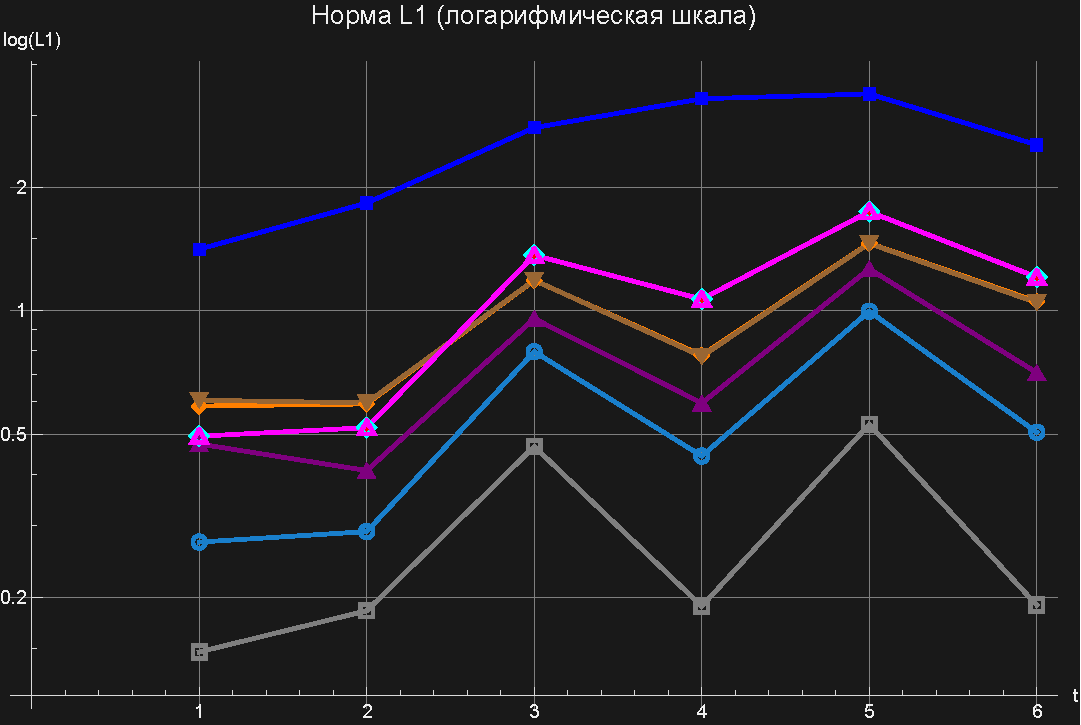
\includegraphics[height=5cm, keepaspectratio]{a_t_log_err_l1.pdf}
		\caption{Логарифмический график ошибок для нормы $L_1$}
	\end{subfigure}
	\hspace{0.05\textwidth}
	\begin{subfigure}[b]{0.45\textwidth}
		\centering
		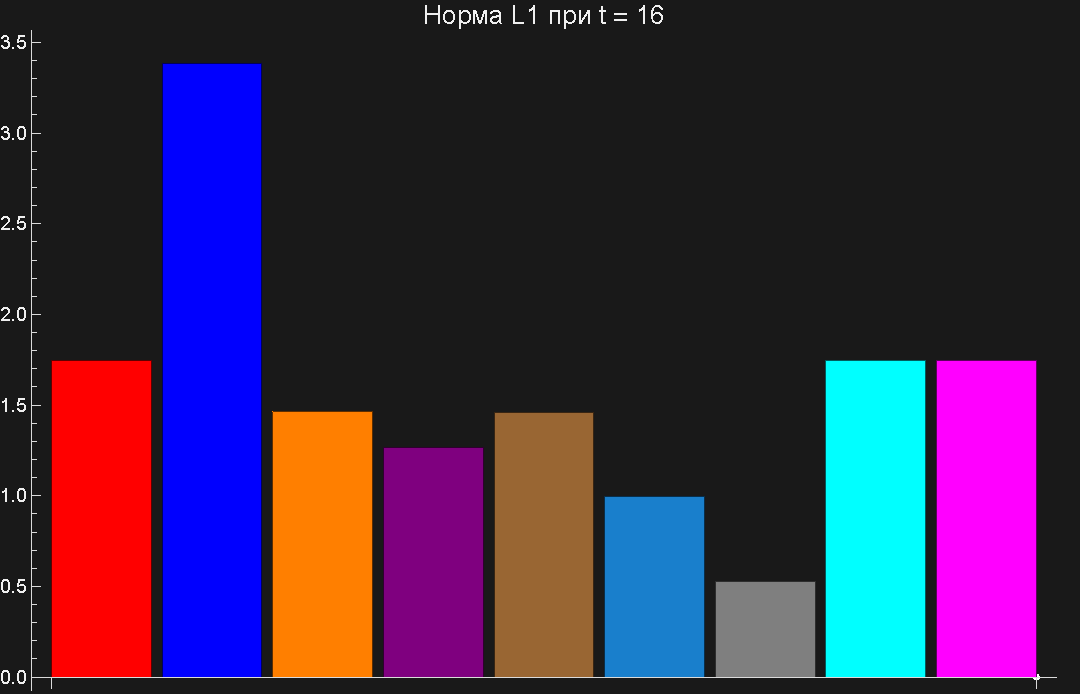
\includegraphics[height=5cm, keepaspectratio]{a_t_bar_err_l1.pdf}
		\caption{Столбчатая диаграмма ошибки для нормы $L_1$ при t=16}
	\end{subfigure}
	
	\vspace{0.5cm}
	
	% Вторая строка
	\begin{subfigure}[b]{0.45\textwidth}
		\centering
		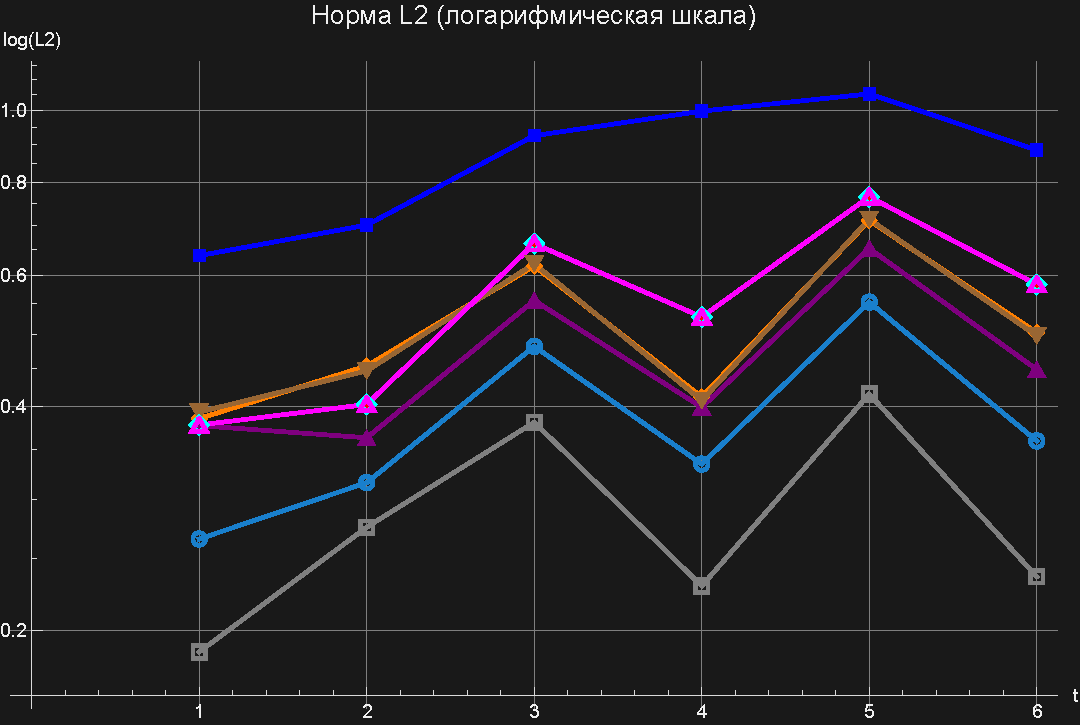
\includegraphics[height=5cm, keepaspectratio]{a_t_log_err_l2.pdf}
		\caption{Логарифмический график ошибок для нормы $L_2$}
	\end{subfigure}
	\hspace{0.05\textwidth}
	\begin{subfigure}[b]{0.45\textwidth}
		\centering
		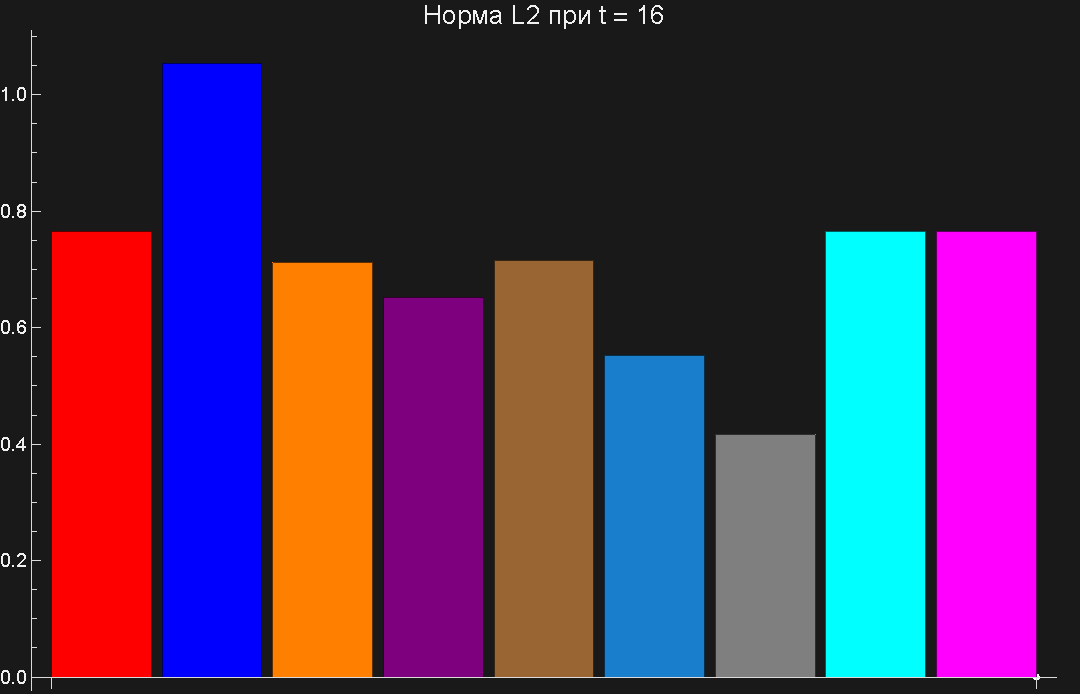
\includegraphics[height=5cm, keepaspectratio]{a_t_bar_err_l2.pdf}
		\caption{Столбчатая диаграмма ошибки для нормы $L_2$ при t=16}
	\end{subfigure}
	
	\vspace{0.5cm}
	
	% Третья строка
	\begin{subfigure}[b]{0.45\textwidth}
		\centering
		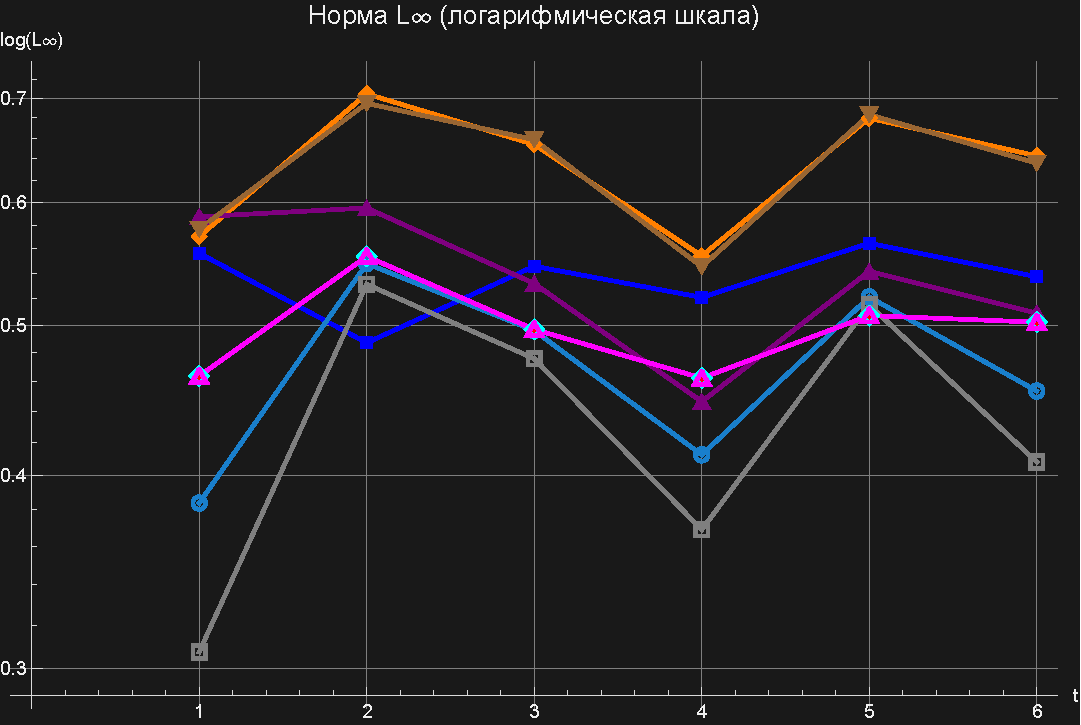
\includegraphics[height=5cm, keepaspectratio]{a_t_log_err_linf.pdf}
		\caption{Логарифмический график ошибок для нормы $L_\infty$}
	\end{subfigure}
	\hspace{0.05\textwidth}
	\begin{subfigure}[b]{0.45\textwidth}
		\centering
		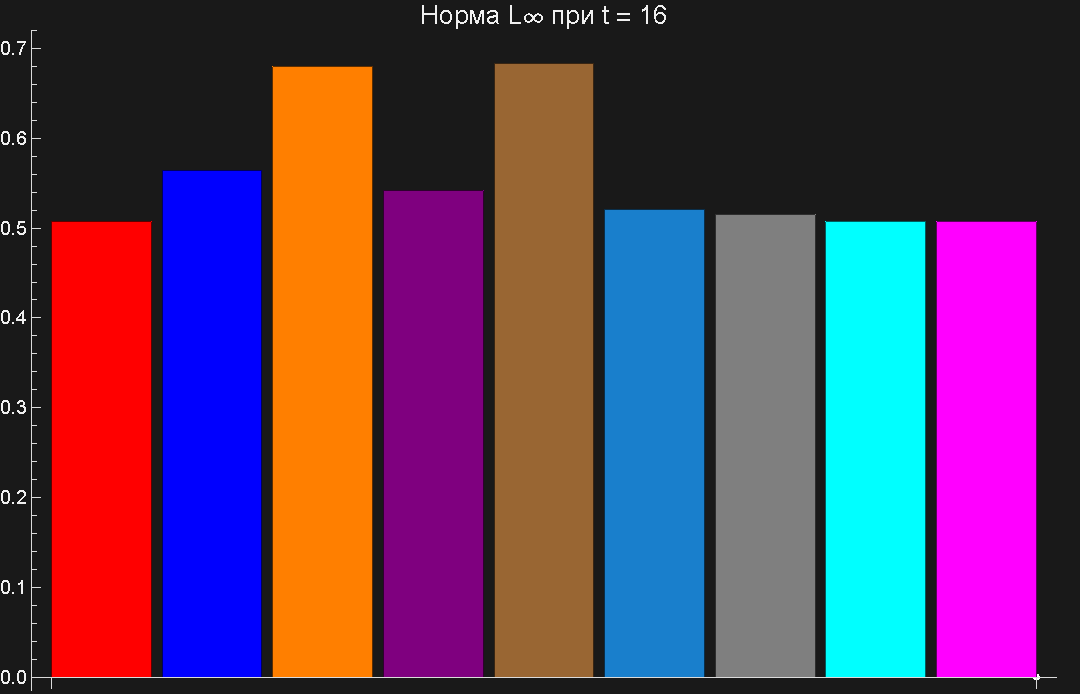
\includegraphics[height=5cm, keepaspectratio]{a_t_bar_err_linf.pdf}
		\caption{Столбчатая диаграмма ошибки для нормы $L_\infty$ при t=16}
	\end{subfigure}
	
	\caption{Сравнение ошибок норм при $a=a(x)$}
\end{figure}

Так же как и в предыдущем случае на логорифмических графиках цифрами обозначены соответствующие временные точки из таблицы.


\section*{{Случай коэффициента, зависящего от времени $(a=a(t))$}}

Параметры аппроксимации для этого случая:
\[
\begin{aligned}
	a(t) &= (-1)^{\lfloor t \rfloor}. \\
	h &= 0.25, \\
	\tau &= 0.05, \\
	x &\in [-10,\,10], \\
	N &= 500.
\end{aligned}
\]

Для данного случая рассматривается не обычная "ступенька", а функция, представляющая собой прямоугольный импульс конечной ширины. При таком коэффициенте скорости профиль не распространяется монотонно в одном направлении, а совершает возвратно-поступательные движения. Другими словами изначальный профиль переодически смещается и возвращается в исходную область. В данном случае использование прямоугольного импульса в качестве начального условия позволяет явно проследить влияние смены направления переноса на устойчивость и точность явных разностных схем.

% --- ЧАСТЬ 1: первые 2 графика ---
\begin{figure}[H]
	\vspace{10pt}
	\centering
	\begin{subfigure}[b]{0.45\textwidth}
		\centering
		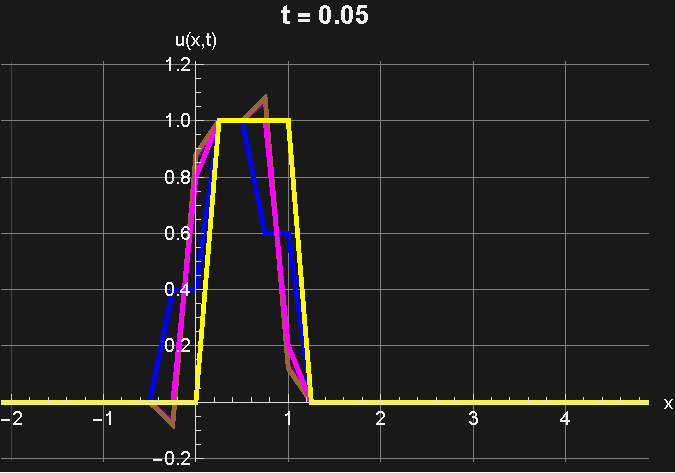
\includegraphics[height=5cm, keepaspectratio]{a_t_t_0_05.pdf}
		\caption{Момент времени t=0.05}
	\end{subfigure}
	\hspace{0.05\textwidth}
	\begin{subfigure}[b]{0.45\textwidth}
		\centering
		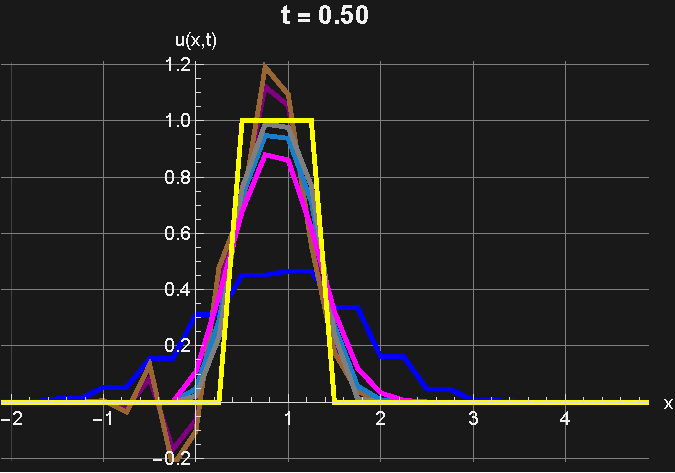
\includegraphics[height=5cm, keepaspectratio]{a_t_t_0_50.pdf}
		\caption{Момент времени t=0.50}
	\end{subfigure}
	
	\caption{Сравнение аппроксимаций для всех схем при $a=a(t)$}
\end{figure}

% --- ЧАСТЬ 2: оставшиеся 4 графика ---
\begin{figure}[H]
	\vspace{10pt}
	\ContinuedFloat % Обязательно: сохраняет номер рисунка прежним
	\centering
	% Вторая строка исходного рисунка
	\begin{subfigure}[b]{0.45\textwidth}
		\centering
		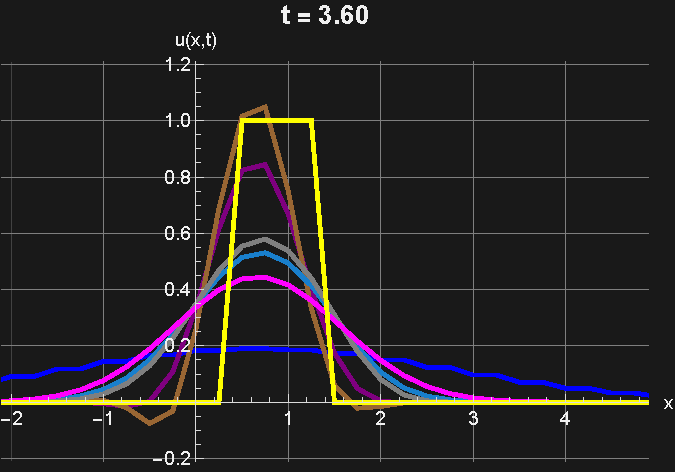
\includegraphics[height=5cm, keepaspectratio]{a_t_t_3_60.pdf}
		\caption{Момент времени t=3.6}
	\end{subfigure}
	\hspace{0.05\textwidth}
	\begin{subfigure}[b]{0.45\textwidth}
		\centering
		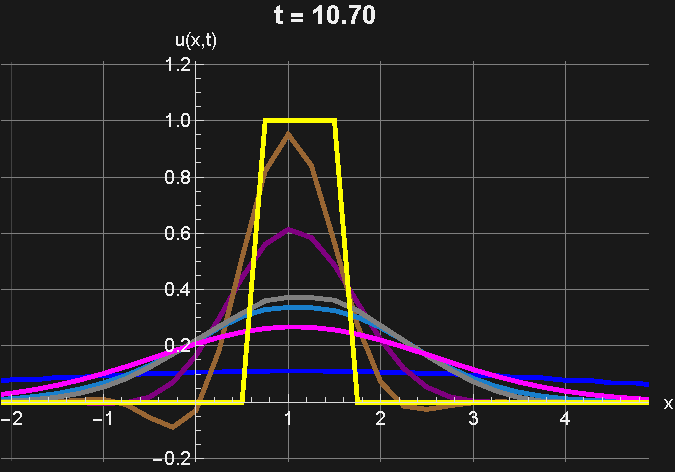
\includegraphics[height=5cm, keepaspectratio]{a_t_t_10_70.pdf}
		\caption{Момент времени t=10.7}
	\end{subfigure}
	
	\vspace{0.5cm}
	
	% Третья строка исходного рисунка
	\begin{subfigure}[b]{0.45\textwidth}
		\centering
		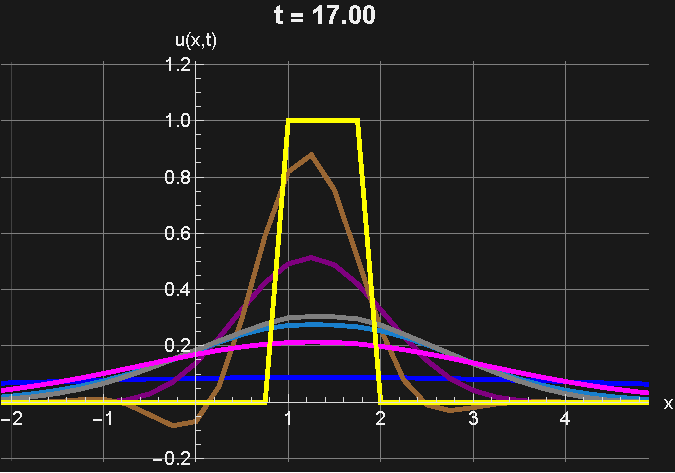
\includegraphics[height=5cm, keepaspectratio]{a_t_t_17.pdf}
		\caption{Момент времени t=17}
	\end{subfigure}
	\hspace{0.05\textwidth}
	\begin{subfigure}[b]{0.45\textwidth}
		\centering
		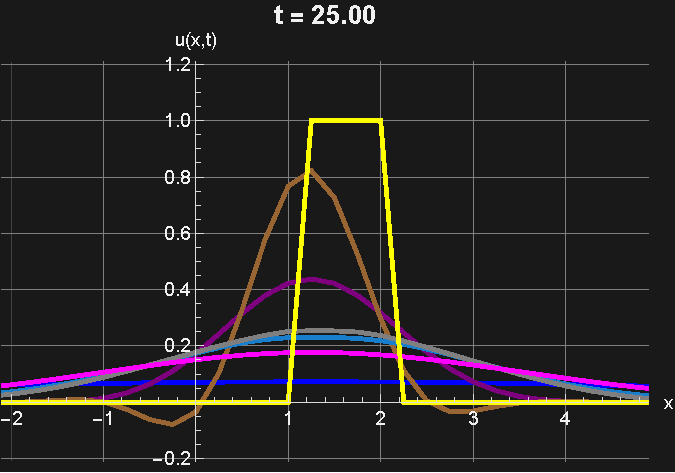
\includegraphics[height=5cm, keepaspectratio]{a_t_t_25.pdf}
		\caption{Момент времени t=25}
	\end{subfigure}
	
	\caption{Сравнение аппроксимаций для всех схем при $a=a(t)$ (продолжение)}
	\label{fig:all_schemes_a_t}
\end{figure}

В случае скорости переноса, переодически меняющей знак, импульс решения, действительно, возвращается в исходную точку по пространственной координате. Однако, такое движение происходит при возврастании времени и это не соответствует движению вдоль одной и той же характеристики в обратном направлении по времени. Отсда следует, что несмотря на возвращение профиля обратно в пространстве, эволюция движения остается однонаправленной по времени.

Важная особенность явных разностных схем заключается в том, что они развиваются строго вперед по времени и не имею возможности перейти обратно к предыдущему временному слою. В результате при каждом возвращении профиля происходит дополнительное накопление численной диссипации, что приводит к постепенному снижению амплитуды решения.

Данный эффект отражен на характеристическом решении рисунка \ref{fig:graph1_a_t}, где отражено, что возврат импульса в пространстве не сопроваждается возвратом по времени. Исходя из всего вышесказанного, можно заключить, что наблюдаемое расхождение с аналитическим решением не свидетельствует о некорректности аппроксимации, а показывает фундаментальное ограничение явных разностных схем при моделировании возвратно-поступательного процесса переноса.

В таблице \ref{tab:norms_small_t} фигурируют нормы ошибок численного решения относительно аналитического решения для различных явных разностных схем при коэффициенте переноса $a=a(t)$, полученные результаты полезны для сравнительного анализа устойчивости и точности схем.

% --- ПЕРВАЯ ЧАСТЬ ТАБЛИЦЫ (L1 и L2) ---
\begin{table}[H]
	\centering
	\caption{Нормы ошибок для всех схем при $a=a(t)$}
	\label{tab:norms_small_t}
	\small
	\adjustbox{max width=\textwidth}{
		\begin{tabular}{|c|c|*{10}{c|}}
			\hline
			\rotatebox{90}{Норма} & $t$
			& \rotatebox{90}{Против Потока }
			& \rotatebox{90}{ЛФ}
			& \rotatebox{90}{ЛВ}
			& \rotatebox{90}{Центр. Вязк.}
			& \rotatebox{90}{Мак-Кормак}
			& \rotatebox{90}{TVD}
			& \rotatebox{90}{MUSCL}
			& \rotatebox{90}{Русанов}
			& \rotatebox{90}{Годунов} \\
			\hline
			
			\multirow{6}{*}{$L_1$}
			& 0.05  & 0.400 & 0.400 & 0.480 & 0.469 & 0.480 & 0.400 & 0.400 & 0.400 & 0.400 \\
			& 0.50  & 0.483 & 1.083 & 0.561 & 0.480 & 0.561 & 0.337 & 0.253 & 0.483 & 0.483 \\
			& 3.60  & 1.170 & 1.624 & 0.543 & 0.644 & 0.543 & 1.023 & 0.944 & 1.170 & 1.170 \\
			& 10.70 & 1.474 & 1.765 & 0.530 & 0.883 & 0.530 & 1.337 & 1.267 & 1.474 & 1.474 \\
			& 17    & 1.578 & 1.760 & 0.655 & 1.046 & 0.655 & 1.456 & 1.399 & 1.578 & 1.578 \\
			& 25    & 1.653 & 1.705 & 0.960 & 1.223 & 0.960 & 1.547 & 1.503 & 1.653 & 1.653 \\
			\hline
			
			\multirow{6}{*}{$L_2$}
			& 0.05  & 0.566 & 0.400 & 0.625  & 0.616 & 0.625 & 0.566 & 0.566 & 0.566 & 0.566 \\
			& 0.50  & 0.373 & 0.652 & 0.413  & 0.372 & 0.413 & 0.285 & 0.236 & 0.373 & 0.373 \\
			& 3.60  & 0.697 & 0.871 & 0.516  & 0.515 & 0.516 & 0.635 & 0.603 & 0.697 & 0.697 \\
			& 10.70 & 0.814 & 0.926 & 0.399  & 0.567 & 0.399 & 0.762 & 0.734 & 0.814 & 0.814 \\
			& 17    & 0.854 & 0.941 & 0.469  & 0.643 & 0.469 & 0.809 & 0.787 & 0.854 & 0.854 \\
			& 25    & 0.882 & 0.950 & 0.689  & 0.732 & 0.689 & 0.845 & 0.828 & 0.882 & 0.882 \\
			\hline
		\end{tabular}
	}
\end{table}

% --- ВТОРАЯ ЧАСТЬ ТАБЛИЦЫ (L_inf) ---
\begin{table}[H]
	\ContinuedFloat % Сохраняет тот же номер таблицы
	\centering
	\caption{Нормы ошибок для всех схем при $a=a(t)$ (продолжение)}
	\small
	\adjustbox{max width=\textwidth}{
		\begin{tabular}{|c|c|*{10}{c|}}
			\hline
			\rotatebox{90}{Норма} & $t$
			& \rotatebox{90}{Против Потока }
			& \rotatebox{90}{ЛФ}
			& \rotatebox{90}{ЛВ}
			& \rotatebox{90}{Центр. Вязк.}
			& \rotatebox{90}{Мак-Кормак}
			& \rotatebox{90}{TVD}
			& \rotatebox{90}{MUSCL}
			& \rotatebox{90}{Русанов}
			& \rotatebox{90}{Годунов} \\
			\hline
			
			\multirow{6}{*}{$L_\infty$}
			& 0.05  & 0.800 & 0.400 & 0.880  & 0.869 & 0.880 & 0.800 & 0.800 & 0.800 & 0.800 \\
			& 0.50  & 0.382 & 0.549 & 0.479  & 0.440 & 0.479 & 0.289 & 0.240 & 0.382 & 0.382 \\
			& 3.60  & 0.638 & 0.814 & 0.690  & 0.617 & 0.690 & 0.586 & 0.560 & 0.638 & 0.638 \\
			& 10.70 & 0.743 & 0.890 & 0.512  & 0.513 & 0.512 & 0.675 & 0.640 & 0.743 & 0.743 \\
			& 17    & 0.793 & 0.912 & 0.592  & 0.580 & 0.592 & 0.733 & 0.704 & 0.793 & 0.793 \\
			& 25    & 0.832 & 0.929 & 0.767  & 0.683 & 0.767 & 0.782 & 0.763 & 0.832 & 0.832 \\
			\hline
		\end{tabular}
	}
\end{table}

% --- ПЕРВАЯ ЧАСТЬ (4 рисунка: L1 и L2) ---
\begin{figure}[H]
	\vspace{10pt}
	\centering
	% Первая строка (L1)
	\begin{subfigure}[b]{0.45\textwidth}
		\centering
		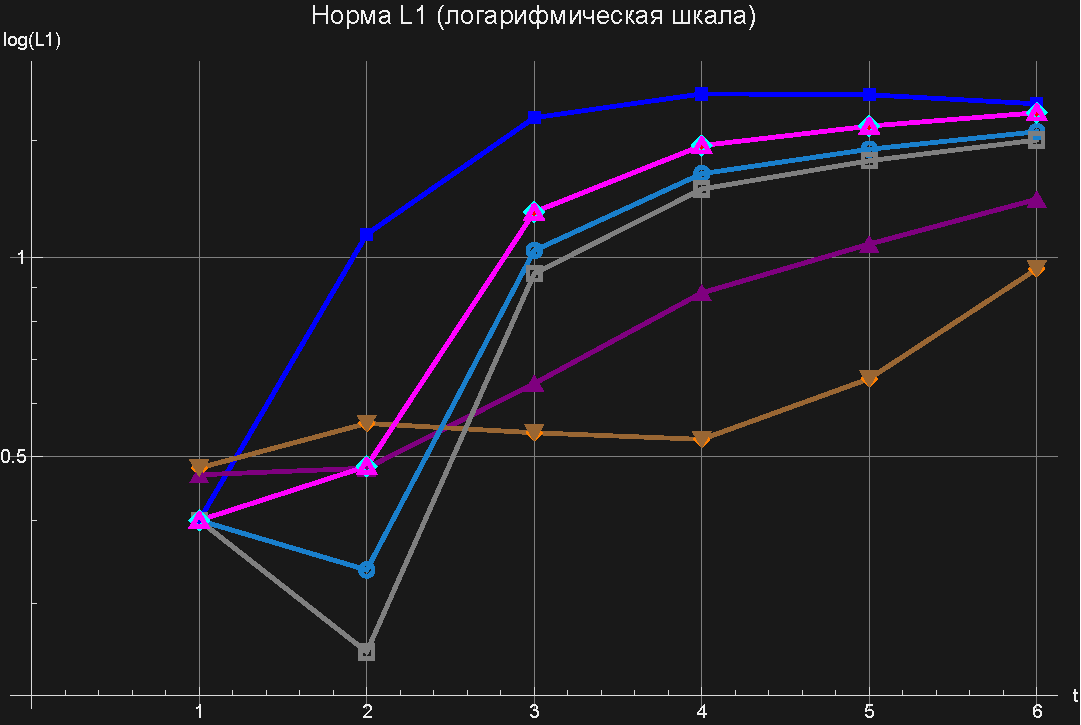
\includegraphics[height=5cm, keepaspectratio]{a_at_log_err_l1.pdf}
		\caption{Логарифмический график ошибок для нормы $L_1$}
	\end{subfigure}
	\hspace{0.05\textwidth}
	\begin{subfigure}[b]{0.45\textwidth}
		\centering
		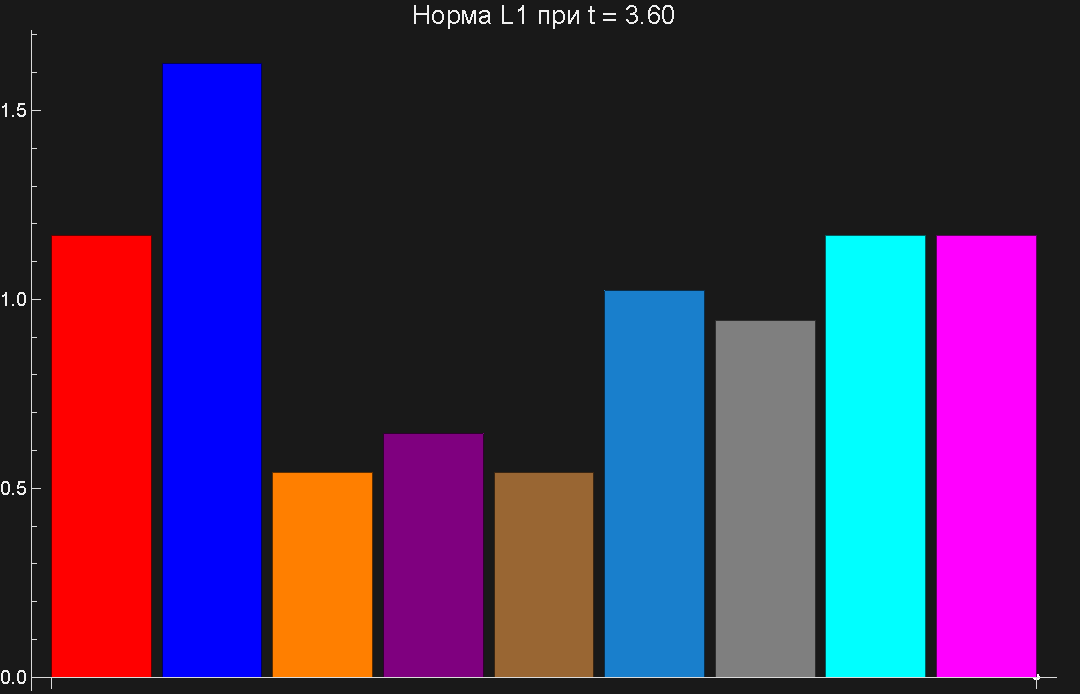
\includegraphics[height=5cm, keepaspectratio]{a_at_bar_err_l1.pdf}
		\caption{Столбчатая диаграмма ошибки для нормы $L_1$ при t=3.6}
	\end{subfigure}
	
	\vspace{0.5cm}
	
	% Вторая строка (L2)
	\begin{subfigure}[b]{0.45\textwidth}
		\centering
		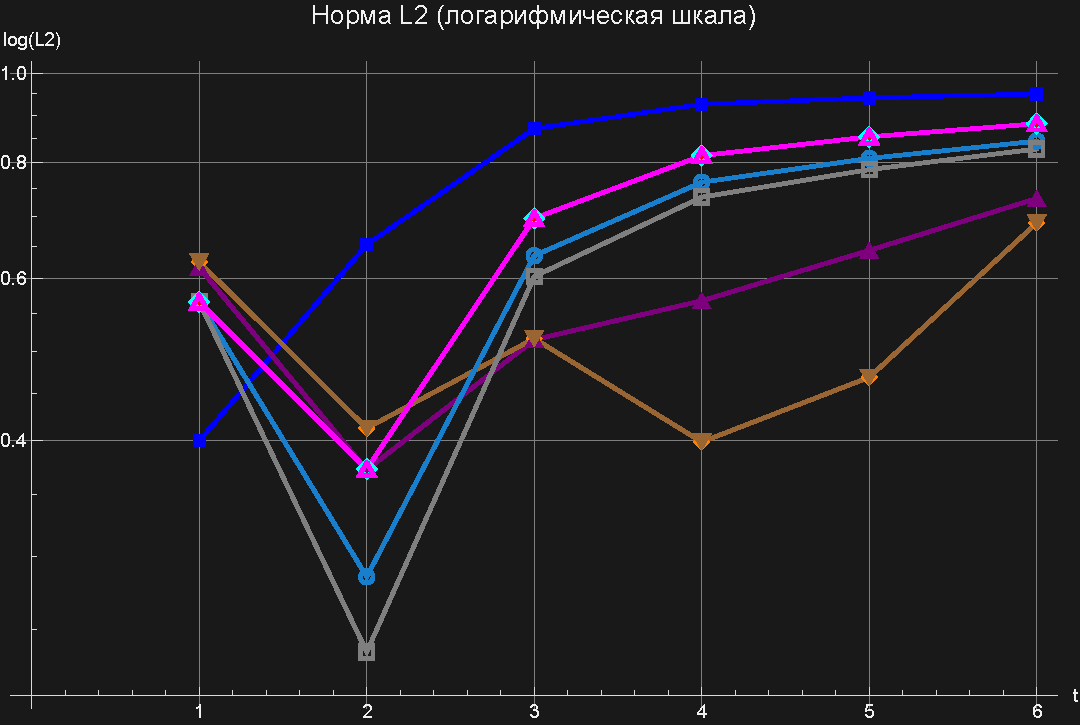
\includegraphics[height=5cm, keepaspectratio]{a_at_log_err_l2.pdf}
		\caption{Логарифмический график ошибок для нормы $L_2$}
	\end{subfigure}
	\hspace{0.05\textwidth}
	\begin{subfigure}[b]{0.45\textwidth}
		\centering
		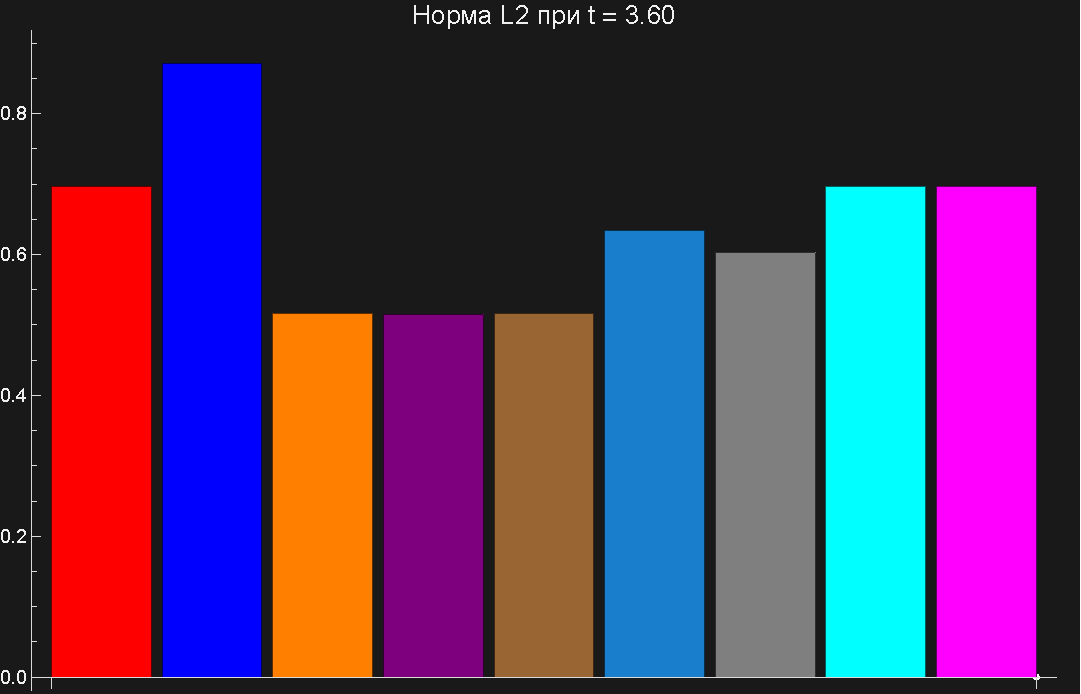
\includegraphics[height=5cm, keepaspectratio]{a_at_bar_err_l2.pdf}
		\caption{Столбчатая диаграмма ошибки для нормы $L_2$ при t=3.6}
	\end{subfigure}
	
	\caption{Сравнение ошибок норм при $a=a(t)$ }
\end{figure}

% --- ВТОРАЯ ЧАСТЬ (2 рисунка: Linf) ---
\begin{figure}[H]
	\vspace{10pt}
	\ContinuedFloat % Сохраняет тот же номер рисунка
	\centering
	% Третья строка (Linf)
	\begin{subfigure}[b]{0.45\textwidth}
		\centering
		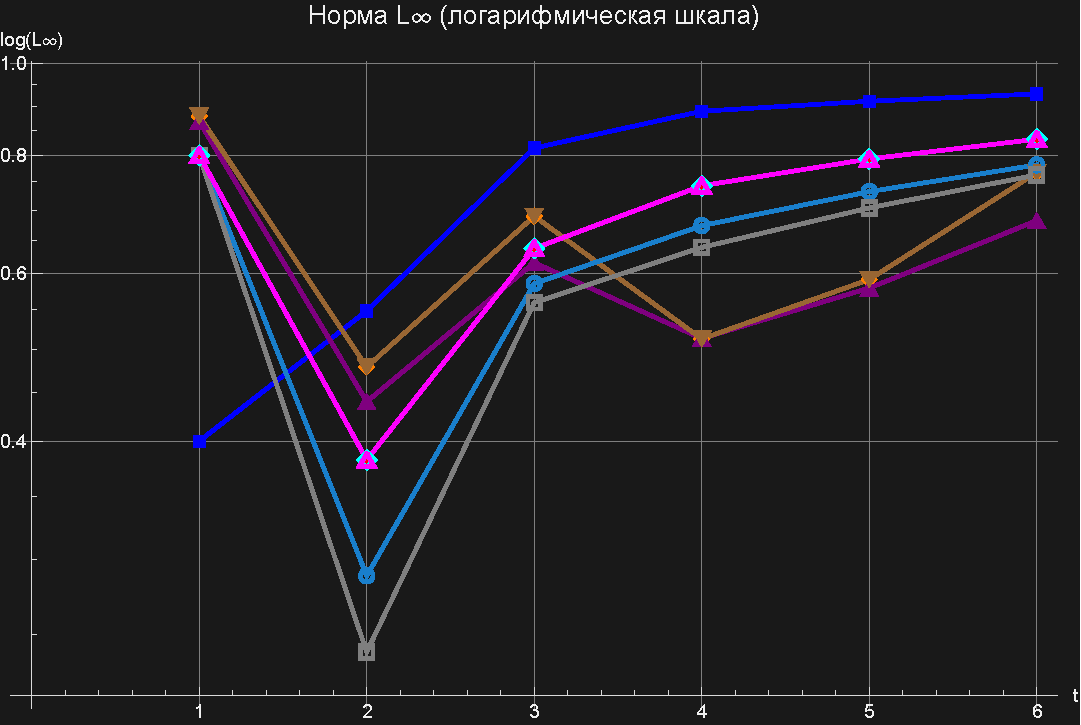
\includegraphics[height=5cm, keepaspectratio]{a_at_log_err_linf.pdf}
		\caption{Логарифмический график ошибок для нормы $L_\infty$}
	\end{subfigure}
	\hspace{0.05\textwidth}
	\begin{subfigure}[b]{0.45\textwidth}
		\centering
		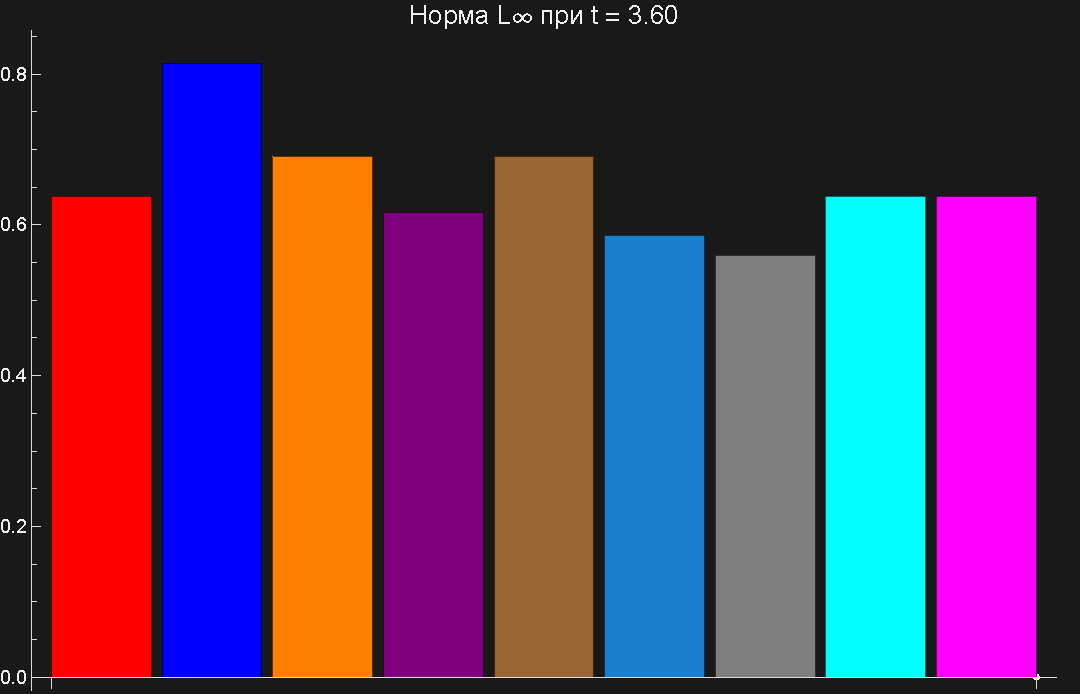
\includegraphics[height=5cm, keepaspectratio]{a_at_bar_err_linf.pdf}
		\caption{Столбчатая диаграмма ошибки для нормы $L_\infty$ при t=3.6}
	\end{subfigure}
	
	\caption{Сравнение ошибок норм при $a=a(t)$ (продолжение)}
	\label{fig:err_comparison_at}
\end{figure}

Так же как и в предыдущем случае на логорифмических графиках цифрами обозначены соответствующие временные точки из таблицы.


\section*{{Случай нестационарного коэффициента $(a(x,t)=x-t)$}}

В случае нестационарной скорости для явных разностных схем, важное внимание следует уделять выбору параметров аппроксимации. Несмотря на то, что схема остается явной, параметры необходимо подбирать так, чтобы они удовлетворяли условию устойчивости на всем рассматриваемом пространственном-временном интервале. Это связано с тем, что при линейной зависимости скорости от координаты и от времени, модуль $a(x,t)$ возврастает при увеличении $x$, $t$, что приводит к локальному росту числа Куранта. При фиксированном пространственном и временном интервалах наибольшее значение скорости достигается на границах определяемой сетки и приводит к повышению критического значения числа Куранта. Исходя из этого параметры $h$, $\tau$ выбиралась таким образом, чтобы они удовлетворяли не строго глобольному условию усточивости, а из локльных требований. 

Для явной схемы условие устойчивости оперделяется из формулы \ref{number:CFL}, этого рассматриваемого случая на расчетной области
\[
\begin{aligned}
	x &\in [-x_{max},\, x_{max}],\\
	t &\in [0,\, t_{max}],
\end{aligned}
\]
Модуль скорости оценивается следующим образом:
\begin{equation}
	\max_{x,t} |a(x,t)| = \max_{x,t} |x - t| \le x_{\max} + t_{\max}.
\end{equation}
Тогда из условия Куранта для явной схемы получаем верхнюю границу шага по времени:
\begin{equation}
	\tau \le \frac{h}{\max|a(x,t)|} = \frac{h}{x_{\max} + t_{\max}}.
\end{equation}
Подставляя значения, принятые для расчёта:
\[
h = 0.5, \quad x_{\max} = 10, \quad t_{\max} = 20,
\]
получаем
\[
\tau \le \frac{0.5}{10 + 20} = \frac{0.5}{30} \approx 0.0167.
\]
Для стабильной и корректной аппроксимации на основной части сетки выбирается шаг времени

\begin{equation}
	\tau = 0.012,
\end{equation}
что обеспечивает коэффициент Куранта примерно равный \(0.72\).
Число временных шагов определяется как

\begin{equation}
	n_{\text{step}} = \left\lfloor \frac{t_{\max}}{\tau} \right\rfloor = \left\lfloor \frac{20}{0.012} \right\rfloor = 1667.
\end{equation}

Таким образом, шаг по времени и количество временных шагов строго вычислены из условия устойчивости и заданного временного интервала расчёта, что обеспечивает корректное поведение явной схемы без чрезмерных осцилляций.


Таким образом парметры аппроксимации имеют вид:
\[
\begin{aligned}
	h &= 0.5, \\
	\tau &= 0.012, \\
	x &\in [-10,\,10], \\
	N &= 1667.
\end{aligned}
\]

Ниже будут представлены рисунки, показывающие графический анализ данного случая коэффициента переноса.

% --- ПЕРВАЯ ЧАСТЬ (4 рисунка: t=0.5, 0.7, 1.5, 2.6) ---
\begin{figure}[H]
	\vspace{10pt}
	\centering
	% Первая строка
	\begin{subfigure}[b]{0.45\textwidth}
		\centering
		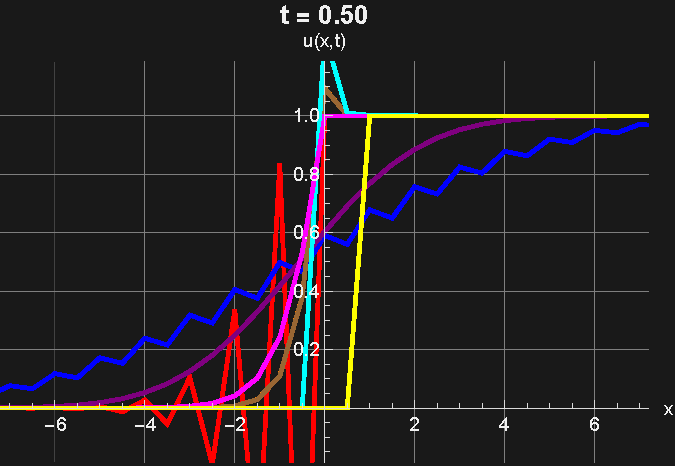
\includegraphics[height=5cm, keepaspectratio]{a_x_t_t_0_50.pdf}
		\caption{Момент времени t=0.5}
		\label{ris:t_0_5}
	\end{subfigure}
	\hspace{0.05\textwidth}
	\begin{subfigure}[b]{0.45\textwidth}
		\centering
		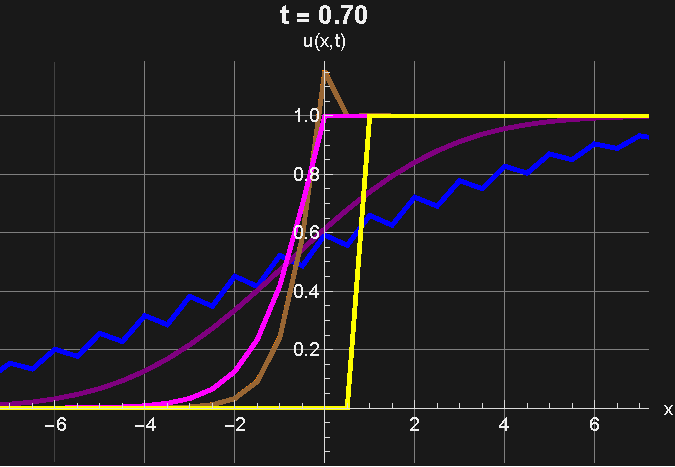
\includegraphics[height=5cm, keepaspectratio]{a_x_t_t_0_7.pdf}
		\caption{Момент времени t=0.7}
	\end{subfigure}
	
	\vspace{0.5cm}
	
	% Вторая строка
	\begin{subfigure}[b]{0.45\textwidth}
		\centering
		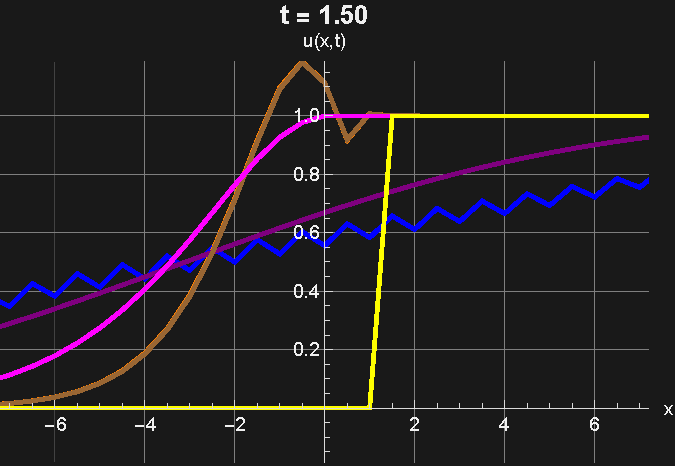
\includegraphics[height=5cm, keepaspectratio]{a_x_t_t_1_50.pdf}
		\caption{Момент времени t=1.5}
	\end{subfigure}
	\hspace{0.05\textwidth}
	\begin{subfigure}[b]{0.45\textwidth}
		\centering
		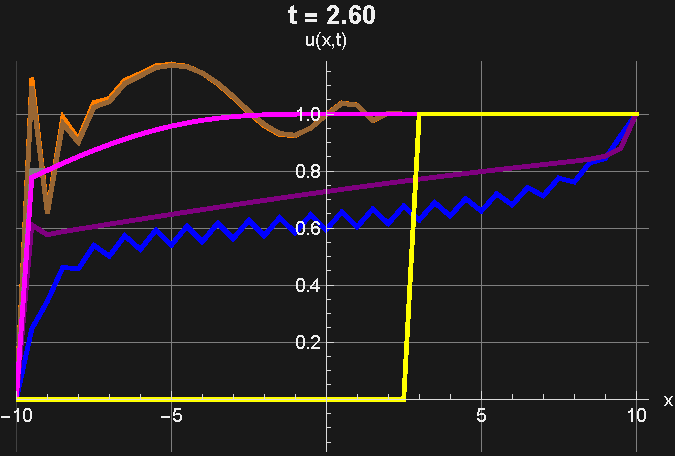
\includegraphics[height=5cm, keepaspectratio]{a_x_t_t_2_6.pdf}
		\caption{Момент времени t=2.6}
	\end{subfigure}
	
	\caption{Сравнение аппроксимаций для всех схем при $a(x,t)=x-t$}
\end{figure}

% --- ВТОРАЯ ЧАСТЬ (2 рисунка: t=6, 10) ---
\begin{figure}[H]
	\vspace{10pt}
	\ContinuedFloat % Сохраняет тот же номер рисунка
	\centering
	% Третья строка (теперь первая в новом блоке)
	\begin{subfigure}[b]{0.45\textwidth}
		\centering
		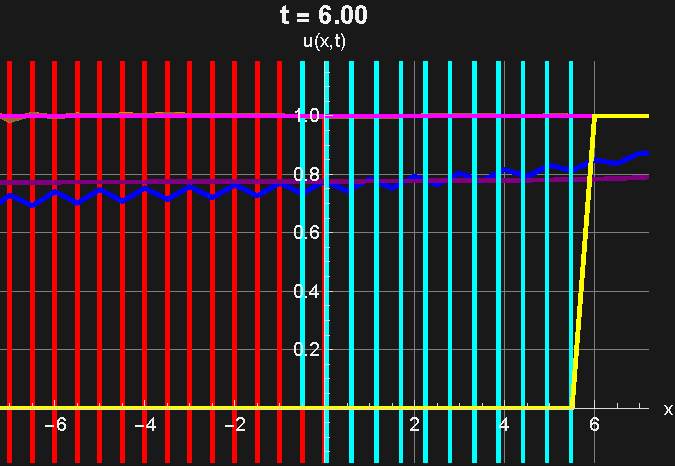
\includegraphics[height=5cm, keepaspectratio]{a_x_t_t_6_0.pdf}
		\caption{Момент времени t=6}
		\label{ris:t_6}
	\end{subfigure}
	\hspace{0.05\textwidth}
	\begin{subfigure}[b]{0.45\textwidth}
		\centering
		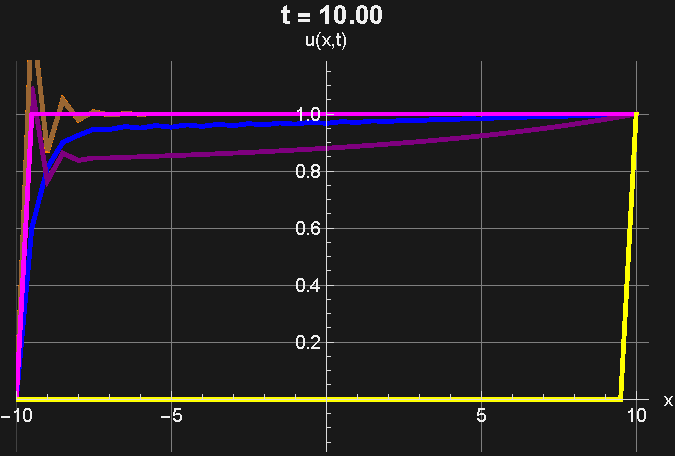
\includegraphics[height=5cm, keepaspectratio]{a_x_t_t_10.pdf}
		\caption{Момент времени t=10}
	\end{subfigure}
	
	\caption{Сравнение аппроксимаций для всех схем при $a(x,t)=x-t$ (продолжение)}
	\label{fig:all_schemes_a_x_t}
\end{figure}

На рисунках \ref{ris:t_0_5} и \ref{ris:t_6} представлены оссциляции создаваемые схемами "Против Потока" и "Русанова", для других рисунков они были убраны, чтобы можно было без помех увидеть другие схемы.
% --- ЧАСТЬ 1: L1 и L2 ---
\begin{table}[H]
	\centering
	\caption{Нормы ошибок для всех схем при $a(x,t)=x-t$}
	\label{tab:norms_a(x,t)}
	\small
	\adjustbox{max width=\textwidth}{
		\begin{tabular}{|c|c|*{10}{c|}}
			\hline
			\rotatebox{90}{Норма} & $t$
			& \rotatebox{90}{Против Потока}
			& \rotatebox{90}{ЛФ}
			& \rotatebox{90}{ЛВ}
			& \rotatebox{90}{Центр. Вязк.}
			& \rotatebox{90}{Мак-Кормак}
			& \rotatebox{90}{TVD}
			& \rotatebox{90}{MUSCL}
			& \rotatebox{90}{Русанов}
			& \rotatebox{90}{Годунов} \\
			\hline
			
			\multirow{6}{*}{$L_1$}
			& 0.5   & 2.616 & 3.497 & 1.313 & 2.006 & 1.312 & 1.472 & 1.472 & 1.146 & 1.472 \\
			& 0.7   & 12.534 & 4.400 & 1.559 & 2.569 & 1.557 & 1.800 & 1.800 & 1.301 & 1.800 \\
			& 1.5   & 5.042e9 & 7.077 & 4.359 & 5.913 & 4.335 & 5.113 & 5.113 & 7.254 & 5.109 \\
			& 2.6   & 3.712e21 & 8.846 & 12.836 & 9.698 & 12.781 & 11.853 & 11.853 & 2.210e3 & 11.840 \\
			& 6     & 1.093e58 & 11.737 & 15.651 & 12.832 & 15.648 & 15.500 & 15.500 & 2.230e17 & 15.500 \\
			& 10    & 6.694e108 & 18.647 & 19.633 & 17.486 & 19.630 & 19.500 & 19.500 & 1.103e45 & 19.500 \\
			\hline
			
			\multirow{6}{*}{$L_2$}
			& 0.5   & 1.483 & 1.072 & 1.087 & 0.898 & 1.086 & 1.085 & 1.085 & 1.153 & 1.085 \\
			& 0.7   & 5.142 & 1.213 & 1.170 & 0.994 & 1.168 & 1.169 & 1.169 & 1.335 & 1.169 \\
			& 1.5   & 4.302e9 & 1.726 & 1.955 & 1.618 & 1.948 & 1.953 & 1.953 & 7.054 & 1.953 \\
			& 2.6   & 4.526e21 & 2.138 & 3.651 & 2.437 & 3.636 & 3.361 & 3.361 & 1.690e3 & 3.358 \\
			& 6     & 1.531e58 & 2.902 & 3.991 & 3.095 & 3.990 & 3.937 & 3.937 & 1.316e17 & 3.937 \\
			& 10    & 9.461e108 & 4.233 & 4.454 & 3.968 & 4.453 & 4.416 & 4.416 & 5.656e44 & 4.416 \\
			\hline
		\end{tabular}
	}
\end{table}

% --- ЧАСТЬ 2: L_inf ---
\begin{table}[H]
	\ContinuedFloat % Сохраняет тот же номер таблицы
	\centering
	\caption{Нормы ошибок для всех схем при $a(x,t)=x-t$ (продолжение)}
	\small
	\adjustbox{max width=\textwidth}{
		\begin{tabular}{|c|c|*{10}{c|}}
			\hline
			\rotatebox{90}{Норма} & $t$
			& \rotatebox{90}{Против Потока}
			& \rotatebox{90}{ЛФ}
			& \rotatebox{90}{ЛВ}
			& \rotatebox{90}{Центр. Вязк.}
			& \rotatebox{90}{Мак-Кормак}
			& \rotatebox{90}{TVD}
			& \rotatebox{90}{MUSCL}
			& \rotatebox{90}{Русанов}
			& \rotatebox{90}{Годунов} \\
			\hline
			
			\multirow{6}{*}{$L_\infty$}
			& 0.5   & 1.107 & 0.591 & 1.095 & 0.691 & 1.094 & 1.000 & 1.000 & 1.280 & 1.000 \\
			& 0.7   & 2.964 & 0.592 & 1.153 & 0.679 & 1.151 & 1.000 & 1.000 & 1.606 & 1.000 \\
			& 1.5   & 5.348 & 0.631 & 1.187 & 0.718 & 1.184 & 1.000 & 1.000 & 9.077 & 1.000 \\
			& 2.6   & 6.330 & 0.678 & 1.174 & 0.765 & 1.170 & 1.000 & 1.000 & 1.704e3 & 1.000 \\
			& 6     & 2.165e58 & 0.831 & 1.445 & 0.924 & 1.437 & 1.000 & 1.000 & 1.064e17 & 1.000 \\
			& 10    & 1.338e109 & 0.998 & 1.360 & 1.094 & 1.352 & 1.000 & 1.000 & 4.010e44 & 1.000 \\
			\hline
		\end{tabular}
	}
\end{table}
Из таблицы \ref{tab:norms_a(x,t)} можно сделать следующие закономерности:
\begin{itemize}
	\item Схемы против потока и Русанова практически с самых малых интервалов времени теряют устойчивость, это связано с численной диффузией и нестабильностью для нестационарного случая.
	\item Схемы Лакса-Фридрихса (ЛФ), Центральная схема с вязкостью, Лакса-Ведроффа (ЛВ), Мак-Кормака, TVD, MUSCL, Годунова сохраняют некую точность на первых шагах и имеют умеренные значения ошибок на всем пространственно-временном интервале, показывая более высокую аппроксимационную точность и контроль осцилляций.
\end{itemize}

\begin{figure}[H]
	\vspace{10pt}
	\centering
	% Первая строка
	\begin{subfigure}[b]{0.45\textwidth}
		\centering
		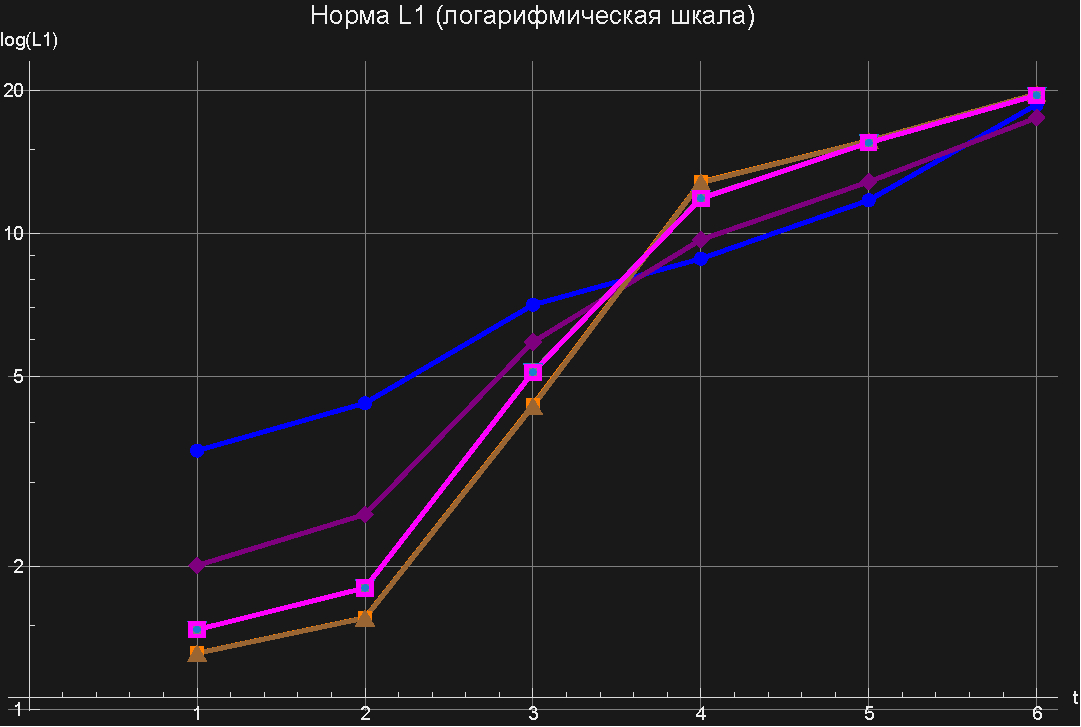
\includegraphics[height=5cm, keepaspectratio]{a_x_t_log_err_l1.pdf}
		\caption{Логарифмический график ошибок для нормы $L_1$}
	\end{subfigure}
	\hspace{0.05\textwidth}
	\begin{subfigure}[b]{0.45\textwidth}
		\centering
		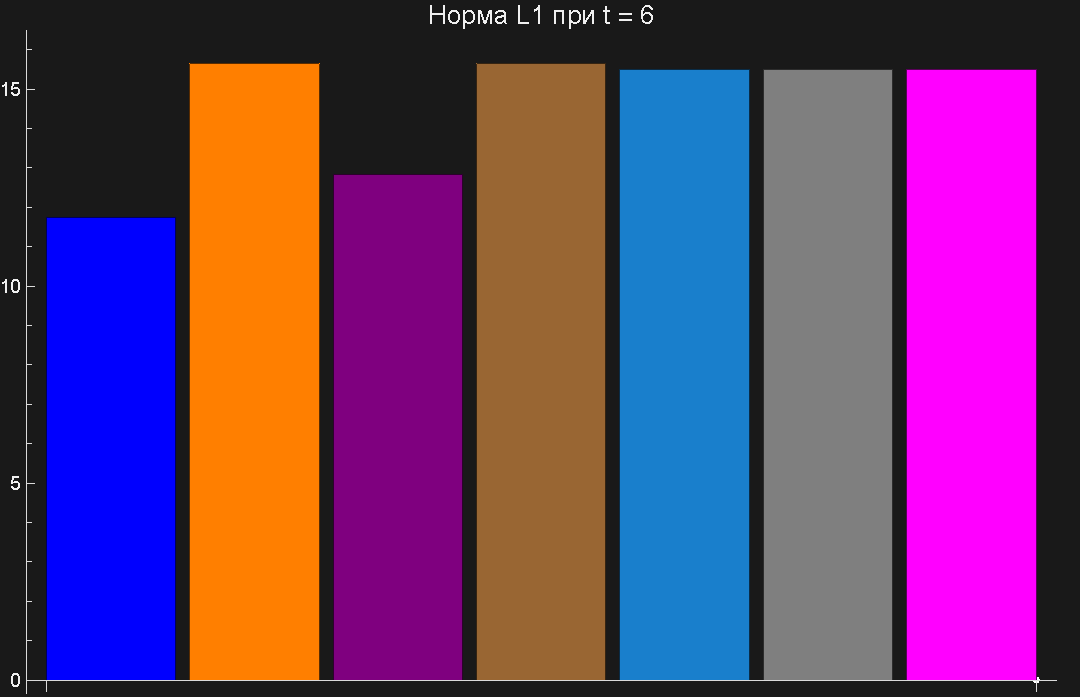
\includegraphics[height=5cm, keepaspectratio]{a_x_t_bar_err_l1.pdf}
		\caption{Столбчатая диаграмма ошибки для нормы $L_1$ при t=6}
	\end{subfigure}
	
	\vspace{0.5cm}
	
	% Вторая строка
	\begin{subfigure}[b]{0.45\textwidth}
		\centering
		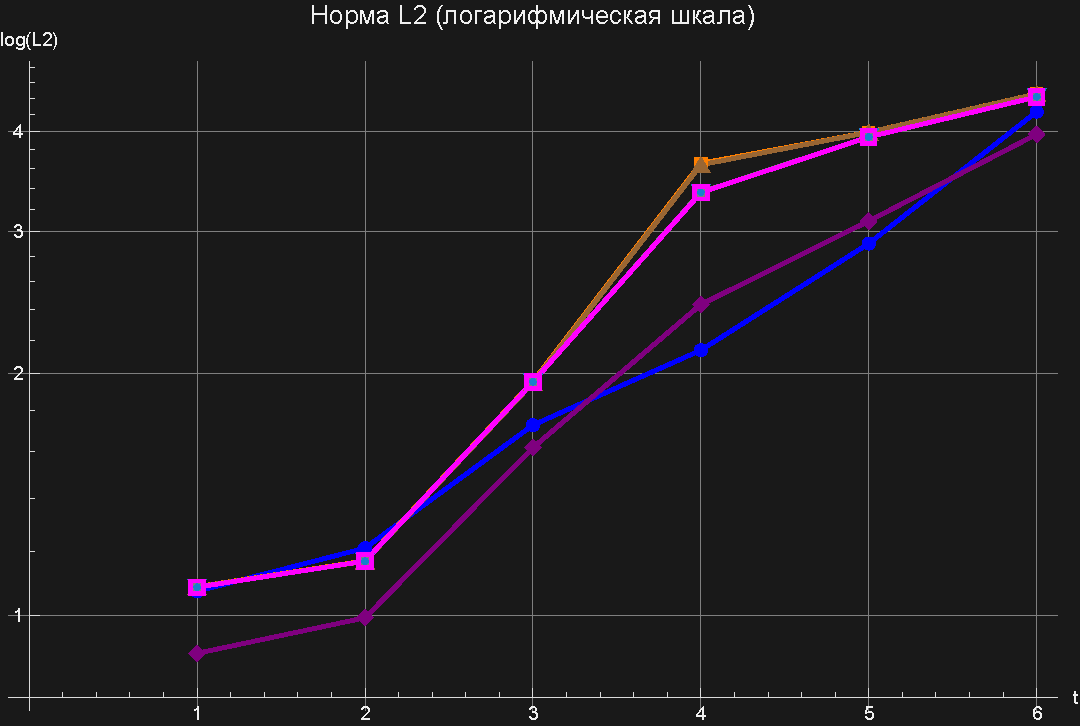
\includegraphics[height=5cm, keepaspectratio]{a_x_t_log_err_l2.pdf}
		\caption{Логарифмический график ошибок для нормы $L_2$}
	\end{subfigure}
	\hspace{0.05\textwidth}
	\begin{subfigure}[b]{0.45\textwidth}
		\centering
		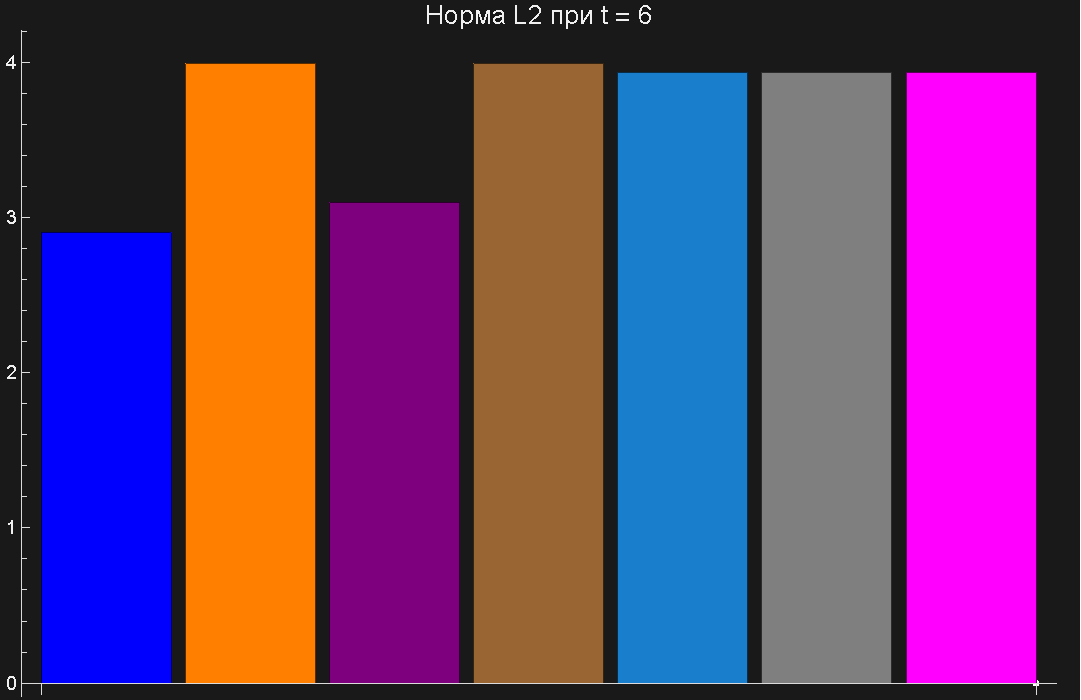
\includegraphics[height=5cm, keepaspectratio]{a_x_t_bar_err_l2.pdf}
		\caption{Столбчатая диаграмма ошибки для нормы $L_2$ при t=6}
	\end{subfigure}
	
	\vspace{0.5cm}
	
	% Третья строка
	\begin{subfigure}[b]{0.45\textwidth}
		\centering
		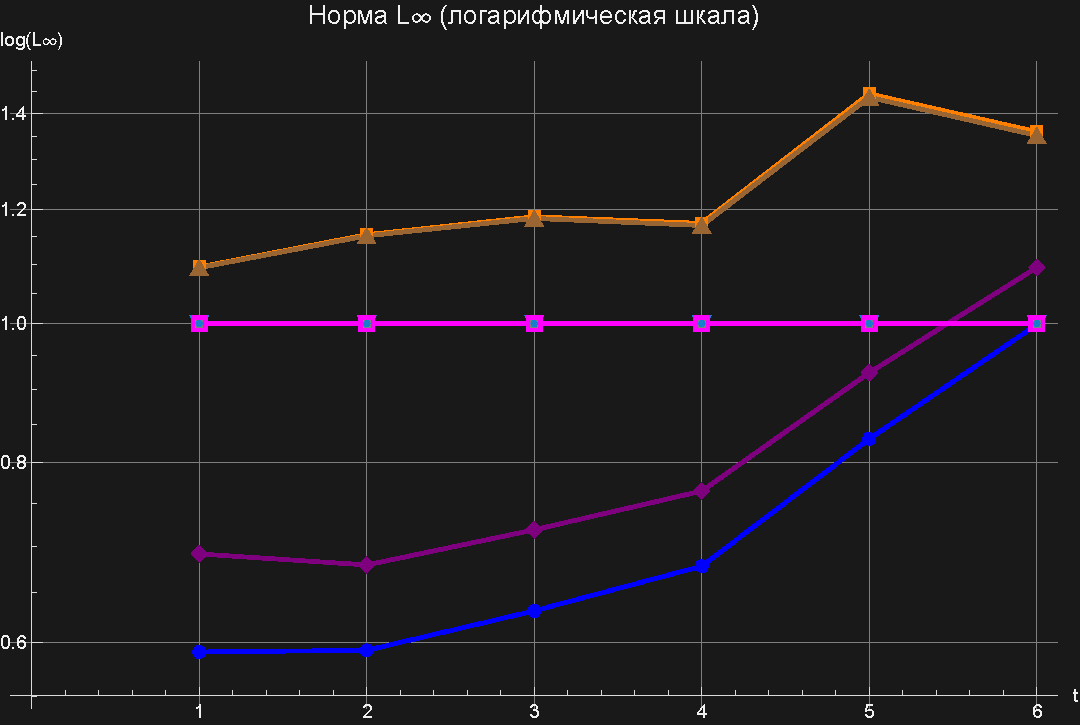
\includegraphics[height=5cm, keepaspectratio]{a_x_t_log_err_linf.pdf}
		\caption{Логарифмический график ошибок для нормы $L_\infty$}
	\end{subfigure}
	\hspace{0.05\textwidth}
	\begin{subfigure}[b]{0.45\textwidth}
		\centering
		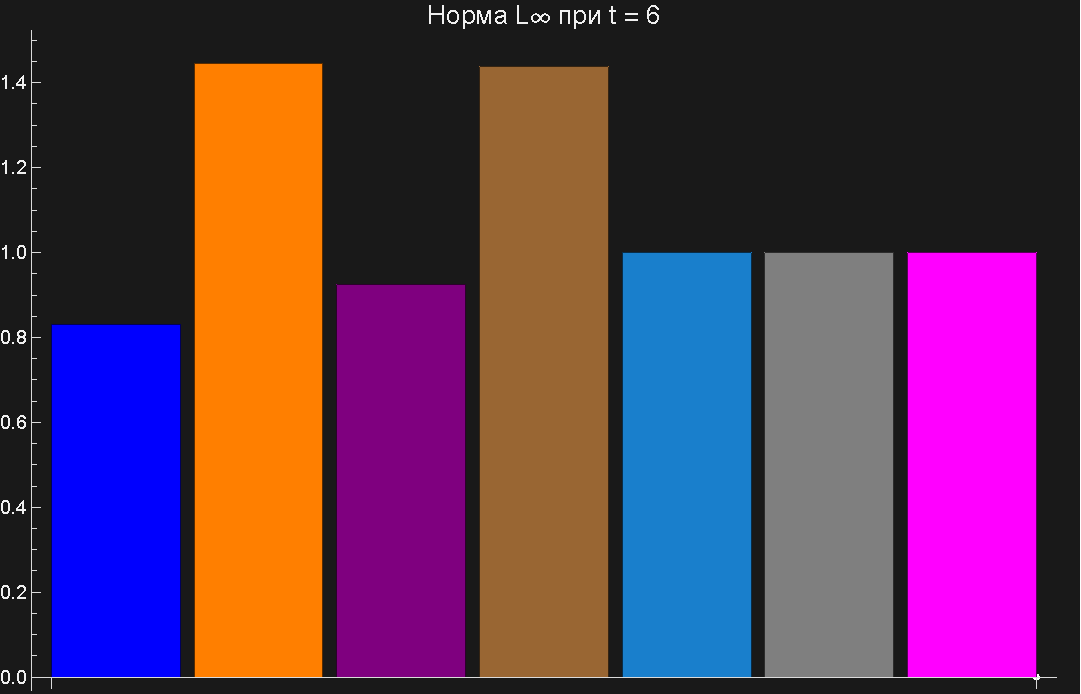
\includegraphics[height=5cm, keepaspectratio]{a_x_t_bar_err_linf.pdf}
		\caption{Столбчатая диаграмма ошибки для нормы $L_\infty$ при t=6}
	\end{subfigure}
	
	\caption{Сравнение ошибок норм при $a(x,t)=x-t$}
\end{figure}

Так же как и в предыдущем случае на логорифмических графиках цифрами обозначены соответствующие временные точки из таблицы. На данных графиках отсутствуют схемы, которые были убраны из рисунка \ref{fig:all_schemes_a_x_t}, так как ошибка слишком большая для этих схем, что мешает на графиках ошибки видеть другие схемы.

Рост ошибки объясняется тем, что для низко-порядковых схем и схем с большой численной диссипацией объясняется тем, что нестационарная скорость в широком диапозоне на расчетной области, что видно из характеристического решения на рисунке \ref{fig:graph1_a_x_t} 

\sectionc{{Итоги аппроксимации явными разностными схемами}}

В данном параграфе были рассмотрены явные разностные схемы для решения уравнения переноса с четырьмя типа коэффициента переноса:

\section*{Постоянный коэффициент $a=const$}

Этот случай является показательным, поскольку показывает стабильное и точное приближение к аналитическому решению, особенно схемы второго порядка(TVD, MUSCL). Низко-порядковые схемы демонстрируют численную диффузию и дисперсию(Мак-Кормак, Лакс-Вендроф, Центральная схема с вязкостью), однако это не влияет на общую картину переноса.

\section*{Коэффициент, зависящий от координаты $a=a(x)$}

При пространственно-зависящем коэффициенте переноса присутствует неравномерное перемещение профиля начальной функции, по этой причине наблюдаются локальные деформации и изменения формы ступеньчатого профиля. Схемы второго порядка(TVD, MUSCL) продолжают демонстрировать высокую точность, а низко-порядковые схемы опять же показывают рассеяние и дисперсии, особенно в областях с резкими градиентами. Схемы же Годунова и Русанова из-за неконсервативности уравнения сводятся к схеме "Против потока".

\section*{Коэффициент, зависящий от времени $a=a(t)$}

Для врмененно-зависящего коэффициента переноса и выбранной функции, профиль решения будет возвращаться в исходную область, что демонстрирует возвратно-поступальное движение. Аппроксимация данного случая абсолютно корректна, даже не смотря на отличие от аналитического решения. Аппроксимация этого случая сопроваждается накоплением численной диссипации при каждом изменении направления переноса, что приводит к уменьшению амплитуды решения.

\section*{Нестационарный коэффициент $a=a(x,t)$}

Случай нестационарной скорости показывает как влияет изменение пространственной и временной пременных на устойчивость явных схем. Для корректной аппроксимации этого случая необходимо учитывать не только глобальное значение числа Куранта, но и локальное значение. Опять же схемы второго порядка показывают более лучшую аппроксимацию, нежели низко-порядковые схемы.

\textit{Анализ, проведенный в данной главе, посвященной аппроксимации явных разностных схем, показывает что они, в целом, могут адекватно аппроксимировать процесс преноса с разными типа его коэффициента. Схемы второго порядка (TVD, MUSCL) лучше показывают себя, когда необходима высокая точность и минизация дисперсии и рассеяния, особенно в задачах с резкими фронтами, как в случае описанным в этой главе. Низко-порядковые схемы применимы в качестве оценки общей картины переноса, но при их использовании требуется учитывать локальные ошибки и численные диффузии.}

\sectionc{{Аппроксимация неявными разностными схемами}}

В данном параграфе будут рассмотрены неявные разностные схемы для уравнения переноса, учитывая разный тип коэффициента переноса. В отличие от явных схем, для неявных нужно решать систему линейных уравнений на каждом временном шаге. Такая система обладает трехдиагональной структурой, что позволяет использовать специализированные методы, отличающиеся от стандартных алгоритмов решения обычных систем линейных уравнений.

Особое внимаение этого параграфа будет уделено анализу данных при числе Куранта больших единицы, поскольку именно в таком случая проявляется преимущестов неявных схем. Условная устойчивость неявных схем позволяет использовать большие временные шаги без потери сходимости. Помимо этого все визуальные представления будут рассматриваться для расширенной пространственной области. Это показывает, что данные схемы можно применять для моделирования процессов переноса на больших интервалах с высокой точностью и устойчивостью.

Исходя из всего вышеперечисленного, можно сказать, что целью данного параграфа является исследование точности, устойчивости и поведение неявных разностных схем при различных типах коэффициента переноса и при числах Куранта, больших единицы, а так же продемонстрировать их преимущество по сравнению с явными схемами.

Для описания неявных схем используются обозначения разностных операторов, введённые в предыдущей главе, а именно формулы \ref{form:oboz1} и \ref{form:oboz2}. 

Помимо этого для неявных схем одним из критериев качества является структура возникающей диагональной матрицы. Наиболее предпочтительным типом матриц является матрица Монте или же М-матрица \cite{kobelkov}.

Квадратная матрица $A=\{a_{ij}\}$ называется М-матрицей, если для нее выполняются следующие условия \cite{kobelkov}.:
\begin{itemize}
	\item Положительность диагональных элементов: $a_{ii} > 0$ для всех $i$;
	\item Неположительность внедиагональных элементов: $a_{ij} \leq 0$ при $i \neq j$;
	\item Диагональное преобладание: Сумма элементов в каждой строке (или столбце) должна быть неотрицательной $\sum_{i \neq j}|a_{ij}| \leq a_{ii}$;
	\item Существование неотрицательной обратной матрицы: Все элементы обратной матрицы $A^{-1}$ должны быть неотрицательны ($a_{ij}^{-1} \geq 0$);
\end{itemize} 

Благодаря М-матрице для неявных схем выполняются следующие свойства, а именно выполнение принципа максимума, то есть решение разностного уравнения не может иметь локальных экстремумов, если их не было в начальных или граничных условиях, выполнение свойства монотонности, то есть решение не может порождать численные осцилляции, выполнение сохранения знака, то есть М-матрица гарантирует, что начальное условие на всех временных шагах остается положительным.
 

\section*{Неявная схема против потока}
\begin{equation}
	u_t + a \, \hat{u}_x^{\mathrm{up}} = 0,    
\end{equation}
где
\[
\hat{u}_x^{\mathrm{up}} =
\begin{cases}
	\hat{u}_{\bar{x}} & a > 0, \\
	\hat{u}_x,      & a < 0.
\end{cases}
\]

Неявная схема против потока является М-матрицей, что объясняет почему она безусловно устойчива и всегда дает гладкое решение без осцилляций (монотонность).

\section*{Неявная центральная схема}
\begin{equation}
	u_t + a\,\hat{u}_{\mathring{x}}=0,
\end{equation}
откуда получаем:
\begin{equation*}
	 \hat{u} \, + \,a\,\frac{\tau}{2h}\,u_{m-1}^{n+1} \, - \,a\,\frac{\tau}{2h}\,\,u_{m+1}^{n+1} = u_m^n 
\end{equation*}

Данная схема не является М-матрицей, так как внедиагональные элементы положительны, что приводит к нарушению монотонности. Ниже на графиках это проявляется в виде сильных осцилляций.

\section*{Неявная схема Лакса-Вендроффа (Регуляризованная схема Лакса-Вендроффа)}
Если взять классическую схему Лакса-Вендроффа и рассмотреть ее на временном слое $n+1$:
\begin{equation*}
	\hat{u} = u_m^n - a\,\frac{\tau}{2h}\left(
	u_{m+1}^{n+1}-u_{m-1}^{n+1} \right)+
	a^2\,\frac{\tau^2}{2h^2}\left(
	u_{m+1}^{n+1} - 2\,u_m^{n+1} + u_{m-1}^{n+1} \right)
\end{equation*}
откуда имеем:
\begin{equation}
	\left( 1 + a^2 \frac{\tau^2}{h^2} \right) u_m^{\,n+1} 
	+ \frac{a\tau}{2h} \left( 1 - \frac{a\tau}{h} \right) u_{m+1}^{\,n+1} 
	- \frac{a\tau}{2h} \left( 1 + \frac{a\tau}{h} \right) u_{m-1}^{\,n+1} = u_m^n.
\end{equation}

Схема не является М-матрицей, так как за счет второго порядка точности она генерирует осцилляции вблизи разрывов. Идет нарушение неположительности внедиагональных элементов.

\section*{Модифицированная неявная схема Кранка–Николсон}

Классическая схема Кранка-Николсона строиться на центральной аппроксимации пространственной производной и имеет симметричный по пространству вид. Однако для уравнения переноса такой подход может приводить к осцилляциям, особенно при наличии разрывов в начальных данных, функциях. Поэтому в работе используется модифицированная неявная схема Кранка-Николсона, в которой пространственная производная аппроксимируется против потока, а усреднение по времени сохраняется
\begin{equation}
	\frac{u_m^{n+1}-u_m^n}{\tau}
	+
	\frac{a}{2}
	\left(
	D_x u_m^{n}
	+
	D_x u_m^{n+1}
	\right)
	=0,
\end{equation}
где $D_x$ определяется следующим образом:
\begin{equation*}
	D_x u_m =
	\begin{cases}
		\dfrac{u_m-u_{m-1}}{h}, & a \ge 0, \\[10pt]
		\dfrac{u_{m+1}-u_m}{h}, & a < 0.
	\end{cases}
\end{equation*}
Если обозначить число Куранта как в формуле \ref{number:CFL}
\begin{equation*}
	\lambda = \dfrac{a\,\tau}{h}.
\end{equation*}
то разностная схема принимает следующий вид.

\text{При} $\lambda \ge 0$:
\begin{equation*}
	\left(1+\frac{\lambda}{2}\right)u_m^{n+1}
	-
	\frac{\lambda}{2}\,u_{m-1}^{n+1}
	=
	\left(1-\frac{\lambda}{2}\right)u_m^{n}
	+
	\frac{\lambda}{2}\,u_{m-1}^{n}
\end{equation*}

\text{При} $\lambda < 0$:
\begin{equation*}
	\left(1-\frac{\lambda}{2}\right)u_m^{n+1}
	+
	\frac{\lambda}{2}\,u_{m+1}^{n+1}
	=
	\left(1+\frac{\lambda}{2}\right)u_m^{n}
	-
	\frac{\lambda}{2}\,u_{m+1}^{n}
\end{equation*}

Данная модификация схемы Кранка-Николсона является М-матрицей, то есть она устойчива и сохраняет монотонность.

\section*{Общая неявная противопоточная схема с учетом направления}
\begin{equation}
	u_t
	+
	\, |a| \,\frac{1}{h} \left[
	\frac{1+\mathrm{sign}(a)}{2} \,	\hat{u}_{\bar{x}}
	+
	\frac{1-\mathrm{sign}(a)}{2} \,\hat{u}_x
	\right] = 0,
\end{equation}
где
\[
\mathrm{sign}(a) =
\begin{cases}
	+1, & a \ge 0, \\
	-1, & a < 0.
\end{cases}
\]

Эта реализация схемы против потока отличается тем, что она автоматически выбирает правильное напрвление аппроксимации производной по пространству в зависимости от знака коэффициента переноса, что является очень полезным при нестационарной скорости переноса. Так же как и неявная против потока, она является М-матрицей.

\section*{Неявная схема с линейной вязкостью}

\begin{equation}
	u_t + a\,\hat{u}_{\mathring{x}} = \frac{\omega\,h^2}{\tau}\,\hat{u}_{\bar{x}x},
\end{equation}
откуда имеем:
\begin{equation*}
	\left(a\,\frac{\tau}{2h} - \omega\right)u_{m+1}^{n+1}\,
	-\,\left(a\,\frac{\tau}{2h} + \omega\right)u_{m-1}^{n+1}\,
	+\,(1+2\omega)\hat{u} = u_m^n
\end{equation*}
Парметр \(0 < \omega < 1\) -- это коэффициент линейной вязкости.

Данная схема позволяет сглаживать численные колебания, которые возникают при неустойчивых численных схемах, что особенно полезно при нестационарных или переменных коэффициентах переноса. 

Тут ситуация обстоит сложнее и все зависит от вязкости, другими словами схема является М-матрицей только при условии, что параметр вязкости $\omega \geq \lambda / 2$

\section*{Неявная схема с вязкостью 4-ого порядка}

\begin{equation}
	u_t + a\,\hat{u}_{\mathring{x}} = \frac{\omega}{8}\left(u_{m+2}^{n+1} - 4u_{m+1}^{n+1} 
	+ 6u_m^{n+1} - 4u_{m-1}^{n+1} + u_{m-2}^{n+1} \right)
\end{equation}

\begin{align*}
	& 
	\frac{\omega}{8} u_{m-2}^{\,n+1} 
	- \Big(\frac{4\omega}{8} + a\,\frac{\tau}{2h} \Big) u_{m-1}^{\,n+1} 
	+ \Big(1 + \frac{6\omega}{8}\Big) u_m^{\,n+1} \notag\\
	&\quad + \Big(- \frac{4\omega}{8} + a\,\frac{\tau}{2h} \Big) u_{m+1}^{\,n+1} 
	+ \frac{\omega}{8} u_{m+2}^{\,n+1} = u_m^n 
\end{align*}
\(0 < \omega < 1\) — коэффициент вязкости четвёртого порядка.  
В данном случае матрица уже не трехдиагональная, а пятидиагональная матрица. Тут для рассмотрения М-матрицы надо смотреть на коэффициенты при $u_{m±1}^{n+1}$, исходя из этого можно заключить, что данная схема не является М-матрицей. Вязкость 4-го порядка хорошо справляется с осцилляциями, но сама структура этой схемы допускает возможность мелких осцилляций.

\section*{Нелинейная вязкостная схема Лакса-Вендроффа}
\begin{equation*}
	u_t + a\,\hat{u}_{\mathring{x}}=
	a^2\,\,\omega\,\tau\,\hat{u}_{\bar{x}x}
\end{equation*}
если обозначить
\begin{equation*}
	\lambda = a\,\frac{\tau}{h}; \quad \nu=\omega\,\frac{a^2\,\tau^2}{2h^2}
\end{equation*}
тогда имеем:
\begin{equation}
	\left(\frac{\lambda}{2}-\nu\right)\,u_{m+1}^{n+1}\,
	+\,(1+2\nu)\,u_{m}^{n+1}-\left(\frac{\lambda}{2} + \nu\right)\,u_{m-1}^{n+1} = u_m^n
\end{equation}

Тут так же надо следить за парметром вязкости, то есть схема является М-матрицей только при условии, что $\nu \geq \lambda / 2$.


\section*{Неявная схема Годунова}

Неявная схема Годунова также учитывает направление волны. В отличие от явной схемы, значение функции на следующем временном слое \(n+1\) вычисляется из системы уравнений, что обеспечивает устойчивость для больших шагов по времени \cite{imranov, kobelkov}.

Численный поток через границу между ячейками выбирается по направлению волны. На границе \(m+1/2\):

\[
F_{m+1/2}^{\,n+1} =
\begin{cases}
	a_{m+1/2}\, u_m^{\,n+1}, & a_{m+1/2} > 0,\\[1mm]
	a_{m+1/2}\, u_{m+1}^{\,n+1}, & a_{m+1/2} < 0,
\end{cases}
\]
на границе \(m-1/2\) соответственно:
\[
F_{m-1/2}^{\,n+1} =
\begin{cases}
	a_{m-1/2}\, u_{m-1}^{\,n+1}, & a_{m-1/2} > 0,\\[1mm]
	a_{m-1/2}\, u_{m}^{\,n+1}, & a_{m-1/2} < 0.
\end{cases}
\]

Значение функции на предыдущем временном слое связано с соседними узлами через формулу:

\begin{equation}
	u_m^n = u_m^{\,n+1} - \frac{\tau}{h} \left(F_{m+1/2}^{\,n+1} - F_{m-1/2}^{\,n+1}\right).
\end{equation}

Раскрывая зависимости от соседних узлов:

\[
u_m^n =
\begin{cases}
	u_m^{\,n+1} - \frac{\tau}{h} \left(a_{m+1/2}\, u_m^{\,n+1} - a_{m-1/2}\, u_{m-1}^{\,n+1}\right), & a_{m+1/2}, a_{m-1/2} > 0,\\[1mm]
	u_m^{\,n+1} - \frac{\tau}{h} \left(a_{m+1/2}\, u_{m+1}^{\,n+1} - a_{m-1/2}\, u_m^{\,n+1}\right), & a_{m+1/2}, a_{m-1/2} < 0,\\[1mm]
	\text{соответствующие комбинации}, & \text{если направления разных знаков}.
\end{cases}
\]

Неявная разностная схема Годунова на верхнем временном слое соответствует системе с М-матрицей. Эта схема - это классический пример монотонной схемы, ее матрица всегда удовлетворяет всем критериям М-матриц.

Так же как в предыдущем параграфе, перед анализом гравической составляющей, будет определено какими цветами будут обозначаться неявные разностные схемы.
\begin{figure}[H]
	\vspace{10pt}
	\centering
	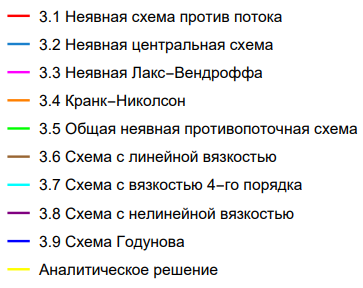
\includegraphics[width=0.45\textwidth,height=6cm,keepaspectratio]{image_2026-01-28_19-58-12.png}
	\caption{Обозначение неявных разностных схем}
	\label{fig:nejavn}
\end{figure}

\section*{{Случай постоянного коэффициента переноса $(a=const)$}}

Как уже ранее отмечалось, неявные схемы преимущественны тем, что для них нет нужды подбирать число Куранта и параметры сетки могут быть абсолютно произвольными.

Так же как и в случае с явными схемами, в данной главе будет использоваться в качестве начальных данных -- функция типа  "ступенька".

Параметры аппроксимации для данного случая:
\[
\begin{aligned}
	a &= 1, \\
	h &= 0.25, \\
	\tau &= 0.5, \\
	x &\in [-280,\,280], \\
	N &= 500.
\end{aligned}
\]

Если проверить число Куранта по формуле \eqref{number:CFL}, то можно действительно убедиться, что данное число превышает единицу:
\[
\lambda = \frac{|a|\tau}{h}=\frac{1 \cdot 0.5}{0.25} = 2\,>\,1
\]


\begin{figure}[H]
	\vspace{10pt}
	\centering
	% Первая строка
	\begin{subfigure}[b]{0.45\textwidth}
		\centering
		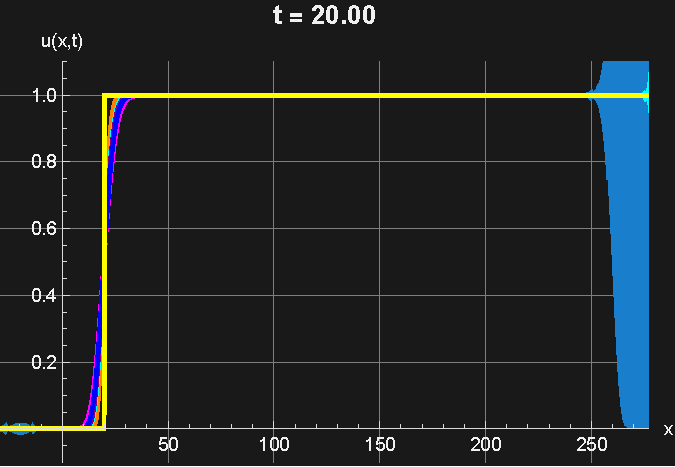
\includegraphics[height=5cm, keepaspectratio]{a_const_nejavn_t_20.pdf}
		\caption{Момент времени t=20}
		\label{fug_lab:t_20}
	\end{subfigure}
	\hspace{0.05\textwidth}
	\begin{subfigure}[b]{0.45\textwidth}
		\centering
		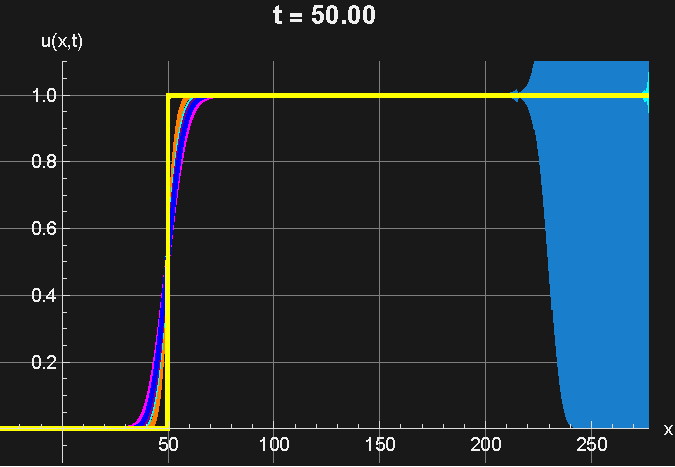
\includegraphics[height=5cm, keepaspectratio]{a_const_nejavn_t_50.pdf}
		\caption{Момент времени t=50}
		\label{fug_lab:t_50}
	\end{subfigure}
	
	\vspace{0.5cm}
	
	% Вторая строка
	\begin{subfigure}[b]{0.45\textwidth}
		\centering
		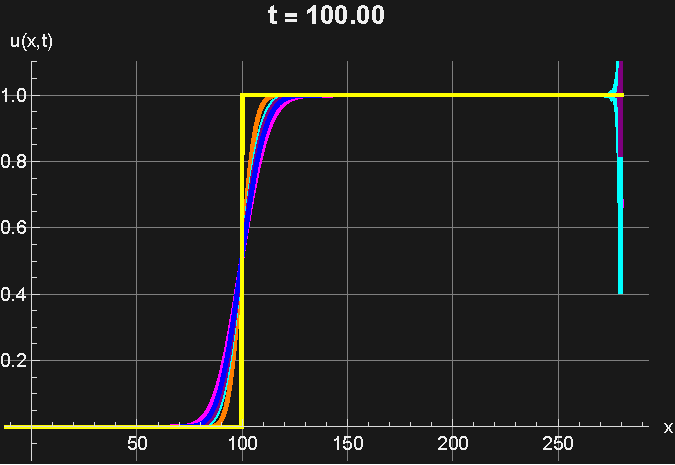
\includegraphics[height=5cm, keepaspectratio]{a_const_nejavn_t_100.pdf}
		\caption{Момент времени t=100}
		\label{fug_lab:t_100}
	\end{subfigure}
	\hspace{0.05\textwidth}
	\begin{subfigure}[b]{0.45\textwidth}
		\centering
		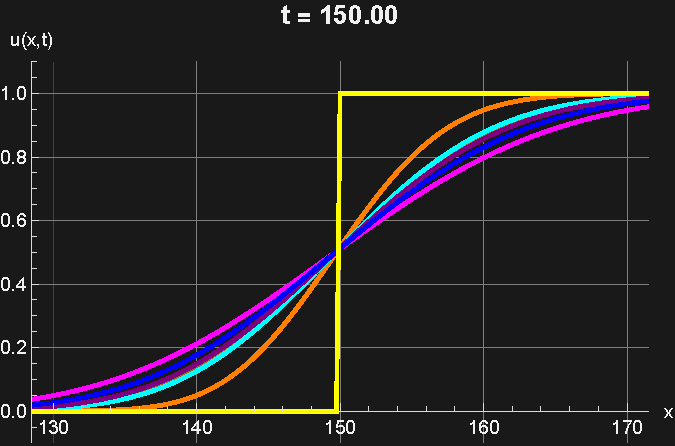
\includegraphics[height=5cm, keepaspectratio]{a_const_nejavn_t_150.pdf}
		\caption{Момент времени t=150}
		\label{fug_lab:t_150}
	\end{subfigure}
	
	\vspace{0.5cm}
	
	% Третья строка
	\begin{subfigure}[b]{0.45\textwidth}
		\centering
		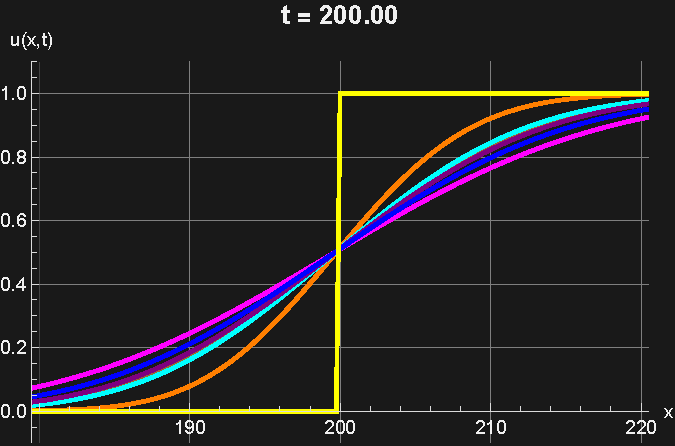
\includegraphics[height=5cm, keepaspectratio]{a_const_nejavn_t_200.pdf}
		\caption{Момент времени t=200}
		\label{fug_lab:t_200}
	\end{subfigure}
	\hspace{0.05\textwidth}
	\begin{subfigure}[b]{0.45\textwidth}
		\centering
		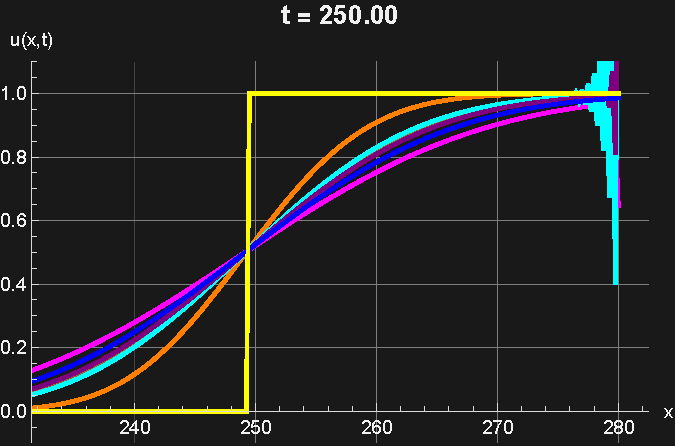
\includegraphics[height=5cm, keepaspectratio]{a_const_nejavn_t_250.pdf}
		\caption{Момент времени t=250}
		\label{fug_lab:t_250}
	\end{subfigure}
	
	\caption{Сравнение аппроксимаций для всех схем при $a=\text{const}$}
	\label{fig:all_schemes_nejavn}
\end{figure}

На рисунках \ref{fug_lab:t_20} и \ref{fug_lab:t_50} видно как для неявной центральной схемы без искусственной вязкости появляются осцилляции, данное поведение связано с отсутствием численного механизма подавления высокочастотных колебаний, именно поэтому в прошлой главе аналог данной схемы был реализован с вязкостью. Также следует отметить, что на последующих рисунках данная схема не приводится, чтобы её осцилляции не затрудняли анализ поведения остальных численных методов. На рисунках \ref{fug_lab:t_150}, \ref{fug_lab:t_200}, \ref{fug_lab:t_250} показана увеличенная сетка. На них отчетливо видно, как неявные схемы сглаживают аналитическое решение, что свидетельствует о проявление диссипативных свойств неявных схем. При увеличении шага по пространству влияние численной диссипации усиливается, что выражается в размывании фронтов и уменьшении амплитуды решения.

Следует подчеркнуть, что несмотря на наличие осцилляций, неявная центральная схема остаётся формально устойчивой при больших числах Куранта, однако получаемое решение теряет физическую корректность из-за отсутствия диссипативного механизма.Данное наблюдение подтверждает, что при практических расчётах неявные схемы целесообразно применять либо в сочетании с искусственной вязкостью, либо в виде аппроксимаций, изначально обладающих направленной диссипацией.

Из таблицы \ref{tab:norms_compact5} можно сделать следующие выводы:
Норма $L_1$ -- отражает суммарную интегральную ошибку по всей области, монотонно возрастает с увеличением времени для всех схем. Это объясняется накоплением численной диффузии и ошибок аппроксимации при длительном счете. Если посмотреть на центральную схему, то ее значения существенно превышают соответствующие значения других схем, что указывает на неустойчивость схемы и наличие осцелляций. Схемы против потока и схема Годунова дают одинаковые соответствующие значения, что подтверждает их эквивалетность для уравнения переноса при постоянном коэффициенте переноса.

\begin{table}[H]
	\centering
	\caption{Нормы ошибок для всех схем при $a=const$}
	\label{tab:norms_compact5}
	\small
	\adjustbox{max width=\textwidth}{
		\begin{tabular}{|c|c|*{10}{c|}}
			\hline
			\rotatebox{90}{Норма} & $t$
			& \rotatebox{90}{Против потока }
			& \rotatebox{90}{Центральная }
			& \rotatebox{90}{ЛВ}
			& \rotatebox{90}{КН}
			& \rotatebox{90}{Общая пртв птк}
			& \rotatebox{90}{Лин. вязкость}
			& \rotatebox{90}{Вяз. 4-го поряд. }
			& \rotatebox{90}{Нелин. вязкость}
			& \rotatebox{90}{Годунов } \\
			\hline
			
			\multirow{6}{*}{$L_1$}
			& 20  & 3.04 & 21.98 & 3.64 & 1.76 & 3.04 & 3.11 & 3.25 & 2.91 & 3.04 \\
			& 50  & 4.88 & 53.99 & 5.76 & 2.82 & 4.88 & 4.68 & 4.75 & 4.55 & 4.88 \\
			& 100 & 6.91 & 105.64 & 8.10 & 3.99 & 6.91 & 6.41 & 6.40 & 6.36 & 6.91 \\
			& 150 & 8.46 & 149.87 & 9.89 & 4.88 & 8.46 & 7.74 & 7.67 & 7.75 & 8.46 \\
			& 200 & 9.77 & 199.87 & 11.41 & 5.64 & 9.77 & 8.87 & 8.74 & 8.93 & 9.77 \\
			& 250 & 10.84 & 249.36 & 12.54 & 6.30 & 10.84 & 9.79 & 9.63 & 9.90 & 10.84 \\
			\hline
			
			\multirow{6}{*}{$L_2$}
			& 20  & 0.95 & 4.28 & 1.03 & 0.72 & 0.95 & 0.98 & 1.04 & 0.93 & 0.95 \\
			& 50  & 1.20 & 6.94 & 1.30 & 0.91 & 1.20 & 1.19 & 1.24 & 1.16 & 1.20 \\
			& 100 & 1.42 & 9.88 & 1.54 & 1.08 & 1.42 & 1.39 & 1.42 & 1.37 & 1.42 \\
			& 150 & 1.57 & 12.11 & 1.70 & 1.20 & 1.57 & 1.52 & 1.54 & 1.51 & 1.57 \\
			& 200 & 1.69 & 14.01 & 1.83 & 1.29 & 1.69 & 1.63 & 1.64 & 1.62 & 1.69 \\
			& 250 & 1.79 & 15.67 & 1.93 & 1.36 & 1.79 & 1.71 & 1.72 & 1.71 & 1.79 \\
			\hline
			
			\multirow{6}{*}{$L_\infty$}
			& 20  & 0.509 & 1.00 & 0.508 & 0.50 & 0.509 & 0.667 & 0.811 & 0.509 & 0.509 \\
			& 50  & 0.505 & 1.00 & 0.505 & 0.50 & 0.505 & 0.667 & 0.811 & 0.505 & 0.505 \\
			& 100 & 0.504 & 1.00 & 0.504 & 0.50 & 0.504 & 0.667 & 0.811 & 0.504 & 0.504 \\
			& 150 & 0.503 & 1.48 & 0.503 & 0.50 & 0.503 & 0.667 & 0.811 & 0.503 & 0.503 \\
			& 200 & 0.503 & 1.49 & 0.503 & 0.50 & 0.503 & 0.667 & 0.811 & 0.503 & 0.503 \\
			& 250 & 0.502 & 1.49 & 0.502 & 0.50 & 0.502 & 0.657 & 0.804 & 0.502 & 0.502 \\
			\hline
	\end{tabular}}
\end{table}


Норма $L_2$ характеризует среднеквадратичную ошибку, данная норма демонстрирует аналогичную тенденцию что и $L_1$. Для устойчивых схем рост ошибки происходит более плавно, тогда как для центральной схемы наблюдается резкое увеличение значений.

Норма $L_\infty$ определяет максимальную локальную ошибку, остается практически постоянной для большинства схем и мало зависит от времени. Это указывает на сохранение максимальной амплитуды численной ошибки, связанной с фронтами численного решения. Для центальной схемы значение данной нормы снова значительнее выше, что подтверждает наличие локальных осцилляций 

\begin{figure}[H]
	\vspace{10pt}
	\centering
	% Первая строка
	\begin{subfigure}[b]{0.45\textwidth}
		\centering
		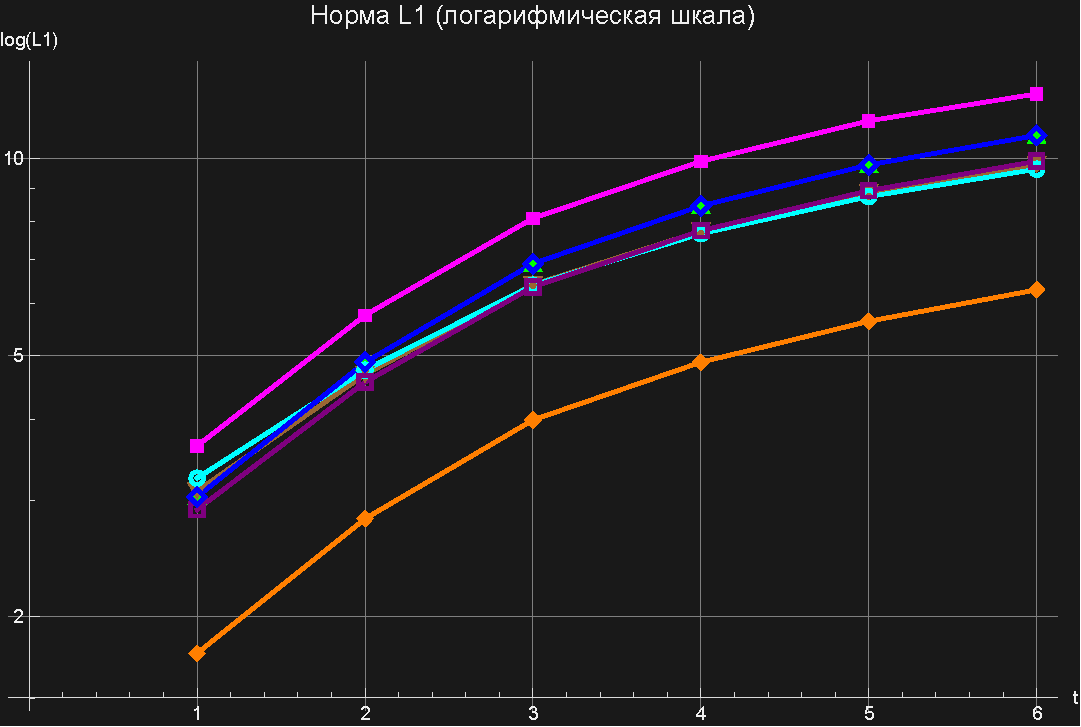
\includegraphics[height=5cm, keepaspectratio]{a_const_t_log_err_l1_nej.pdf}
		\caption{Логарифмический график ошибок для нормы $L_1$}
	\end{subfigure}
	\hspace{0.05\textwidth}
	\begin{subfigure}[b]{0.45\textwidth}
		\centering
		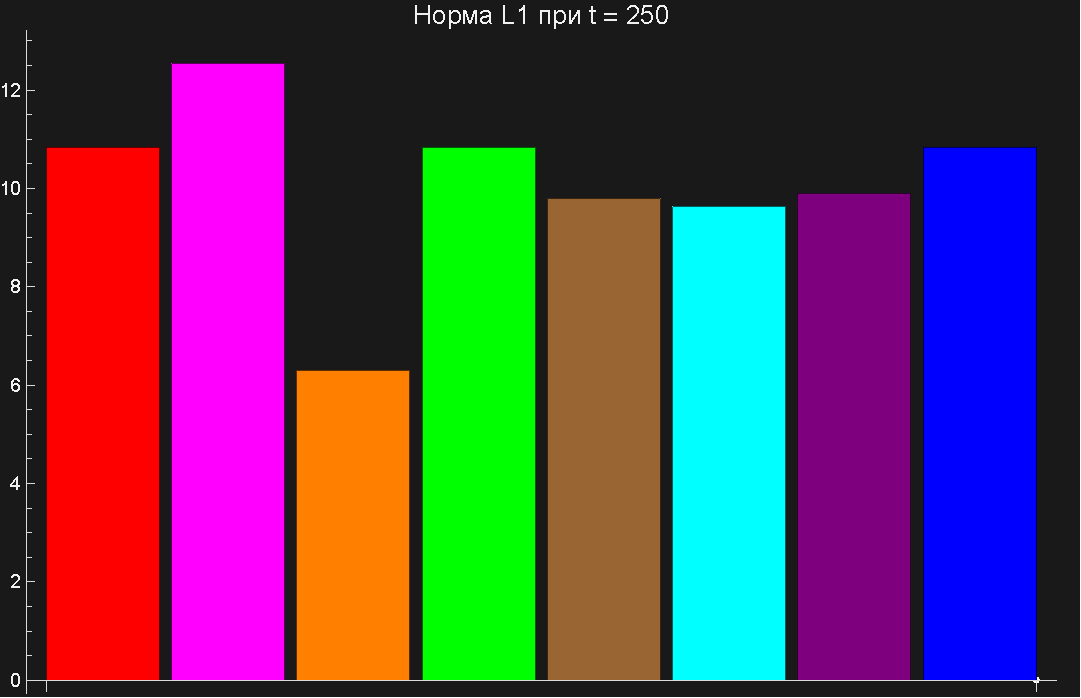
\includegraphics[height=5cm, keepaspectratio]{a_const_t_bar_err_l1_nej.pdf}
		\caption{Столбчатая диаграмма ошибки для нормы $L_1$ при t=250}
	\end{subfigure}
	
	\vspace{0.5cm}
	
	% Вторая строка
	\begin{subfigure}[b]{0.45\textwidth}
		\centering
		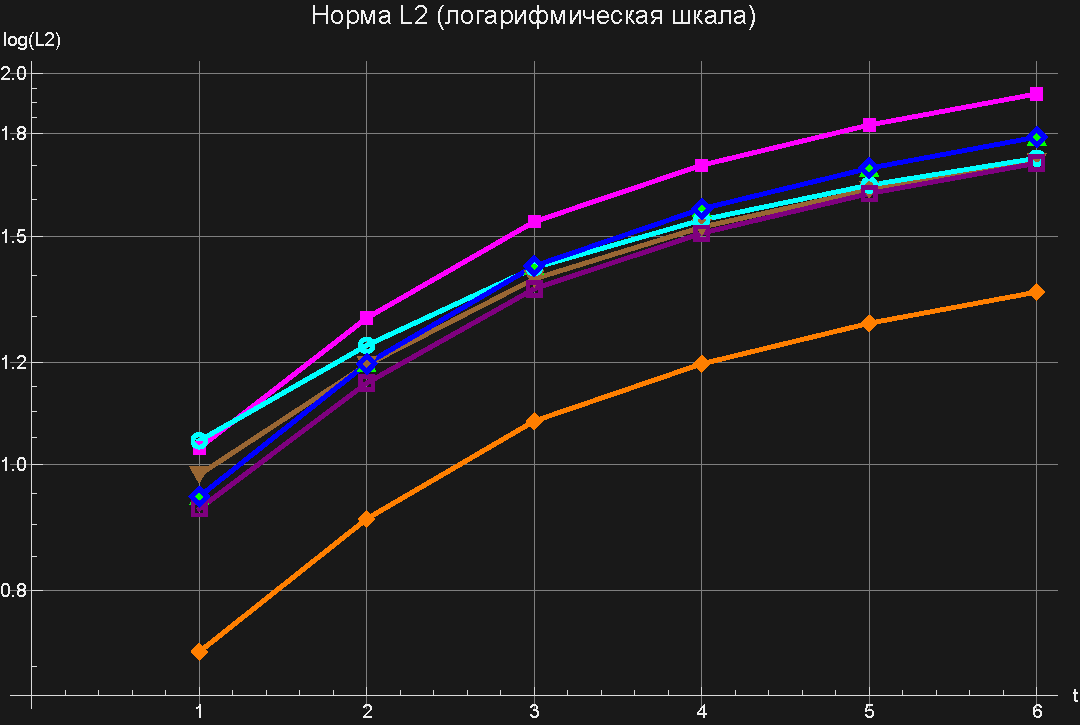
\includegraphics[height=5cm, keepaspectratio]{a_const_t_log_err_l2_nej.pdf}
		\caption{Логарифмический график ошибок для нормы $L_2$}
	\end{subfigure}
	\hspace{0.05\textwidth}
	\begin{subfigure}[b]{0.45\textwidth}
		\centering
		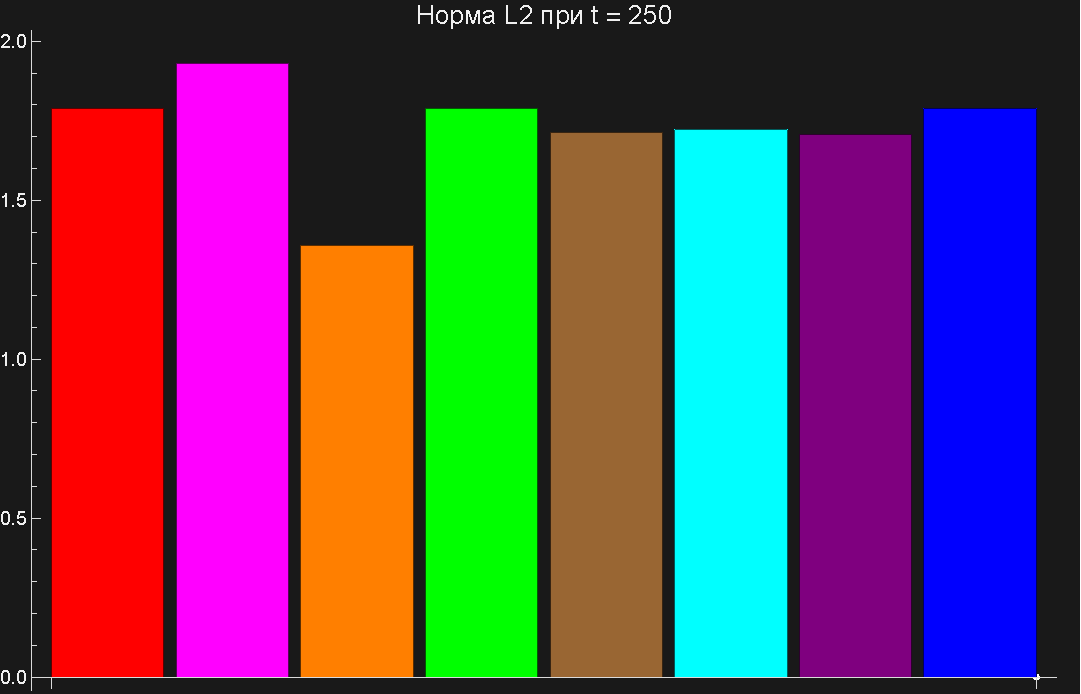
\includegraphics[height=5cm, keepaspectratio]{a_const_t_bar_err_l2_nej.pdf}
		\caption{Столбчатая диаграмма ошибки для нормы $L_2$ при t=250}
	\end{subfigure}
	
	\vspace{0.5cm}
	
	% Третья строка
	\begin{subfigure}[b]{0.45\textwidth}
		\centering
		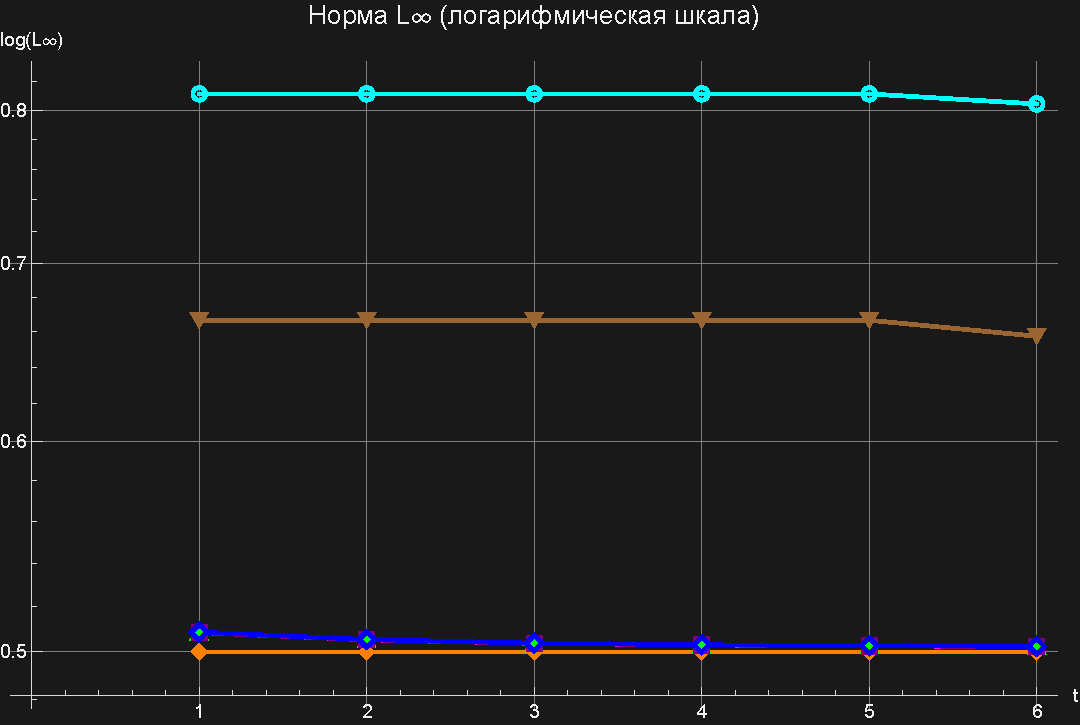
\includegraphics[height=5cm, keepaspectratio]{a_const_t_log_err_linf_nej.pdf}
		\caption{Логарифмический график ошибок для нормы $L_\infty$}
	\end{subfigure}
	\hspace{0.05\textwidth}
	\begin{subfigure}[b]{0.45\textwidth}
		\centering
		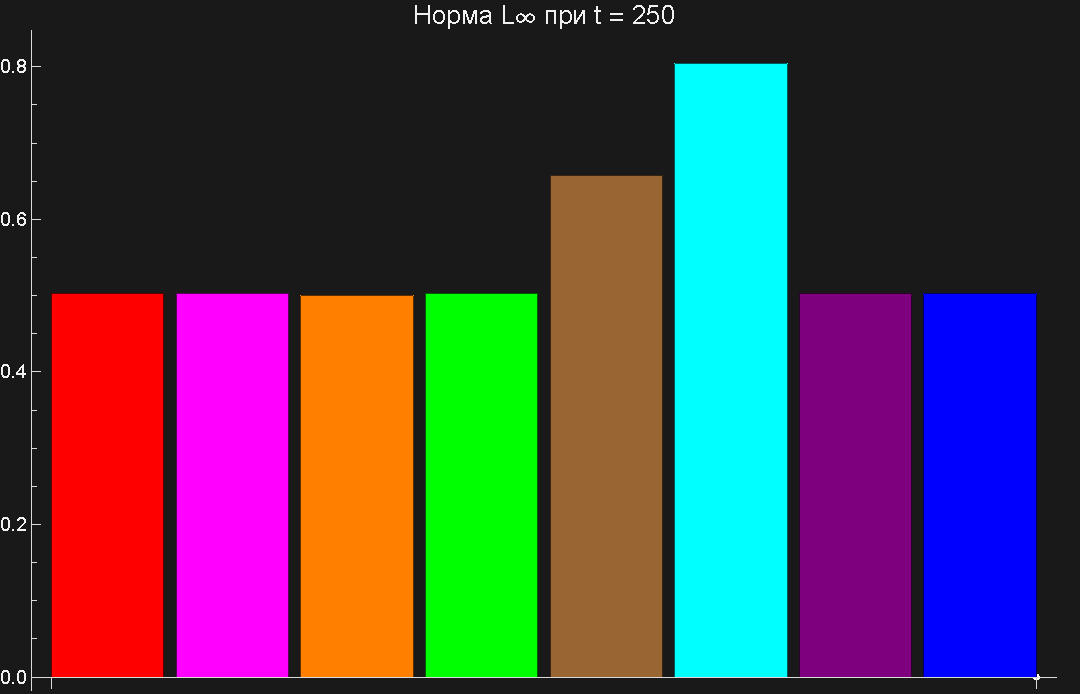
\includegraphics[height=5cm, keepaspectratio]{a_const_t_bar_err_linf_nej.pdf}
		\caption{Столбчатая диаграмма ошибки для нормы $L_\infty$ при t=250}
	\end{subfigure}
	
	\caption{Сравнение ошибок норм при  $a=\text{const}$}
\end{figure}  

В целом по данным значениям норм можно сказать, что при постоянном коэффициенте переноса устойчивые противопоточные и консервативные схемы демонстрируют предсказуемое и согласованное поведение, тогда как центальная схема без стабилизации оказывается непригодной для длительного расчета.

\section*{{Случай коэффициента, зависящего от пространства $(a=a(x))$}}

Параметры аппроксимации для данного случая выглядят следующим образом:
\[
\begin{aligned}
	a(x) &= 1\,+\,\frac{1}{2}\sin(x) , \\
	h &= 0.25, \\
	\tau &= 0.5, \\
	x &\in [-280,\,280], \\
	N &= 500.
\end{aligned}
\]

Для графиков, представленных на рисунке \ref{fig:all_schemes_nejavn_a_x}, исключена центральная схема, так как из рисунка \ref{fug_lab:a_x_t_20} отчётливо проявляются осцелляции. Следует отметить, что с увеличением времени, характер численного решения для данного случая коэффициента переноса усложняется. Схемы помимо диссипативных свойст, присущих неявным схемам, присутствуют волновые колебания аппроксимирующих решений -- это объясняется характером функции $a=a(x)$, ее неоднородной скоростью переноса и локальными изменениями. При этом диссипация неявных разностных схем приводит к сглаживанию фронтов решения, однако полностью подавить волновое искажение, возникающее в результате переменного коэффициента, не представляется возможности. В остальном же все наблюдения схожи со случаем постоянного коэффициента переноса

\begin{figure}[H]
	\vspace{10pt}
	\centering
	% Первая строка
	\begin{subfigure}[b]{0.45\textwidth}
		\centering
		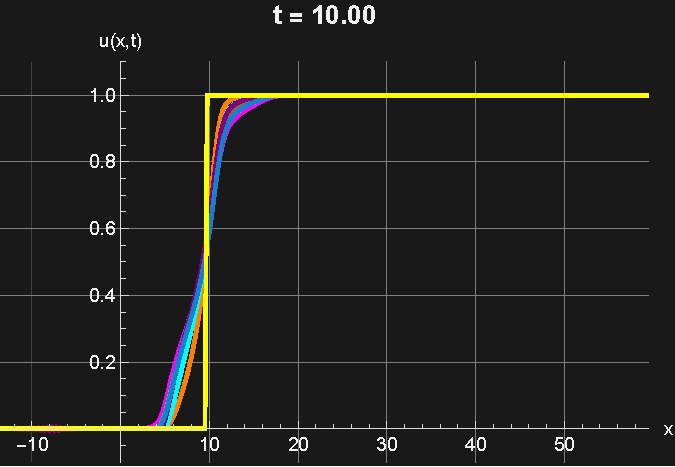
\includegraphics[height=5cm, keepaspectratio]{a_x_nejavn_t_10.pdf}
		\caption{Момент времени t=10}
	\end{subfigure}
	\hspace{0.05\textwidth}
	\begin{subfigure}[b]{0.45\textwidth}
		\centering
		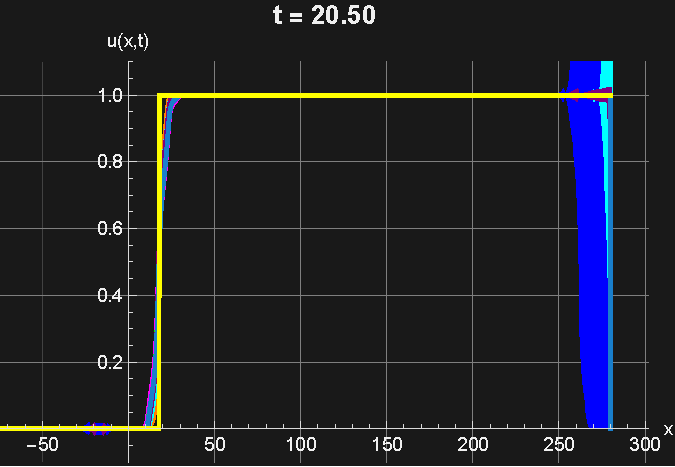
\includegraphics[height=5cm, keepaspectratio]{a_x_nejavn_t_20.pdf}
		\caption{Момент времени t=20}
		\label{fug_lab:a_x_t_20}
	\end{subfigure}
	
	\vspace{0.5cm}
	
	% Вторая строка
	\begin{subfigure}[b]{0.45\textwidth}
		\centering
		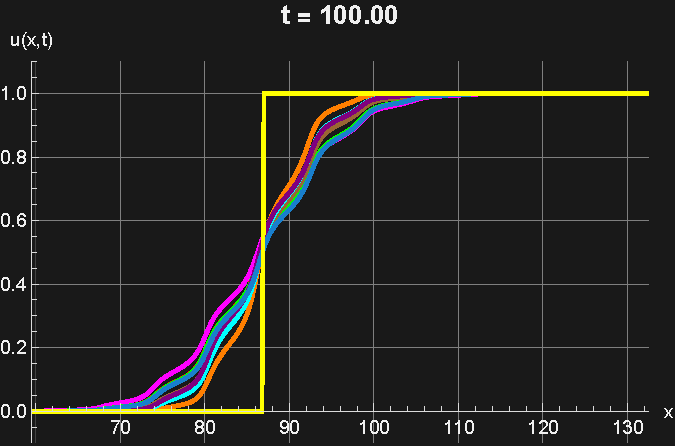
\includegraphics[height=5cm, keepaspectratio]{a_x_nejavn_t_100.pdf}
		\caption{Момент времени t=100}
	\end{subfigure}
	\hspace{0.05\textwidth}
	\begin{subfigure}[b]{0.45\textwidth}
		\centering
		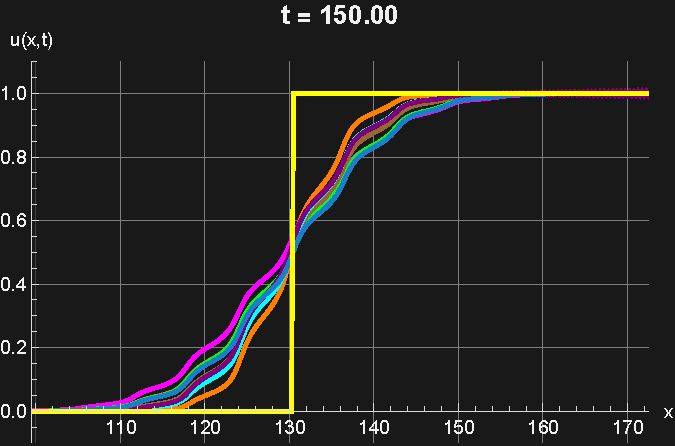
\includegraphics[height=5cm, keepaspectratio]{a_x_nejavn_t_150.pdf}
		\caption{Момент времени t=150}
	\end{subfigure}
	
	\vspace{0.5cm}
	
	% Третья строка
	\begin{subfigure}[b]{0.45\textwidth}
		\centering
		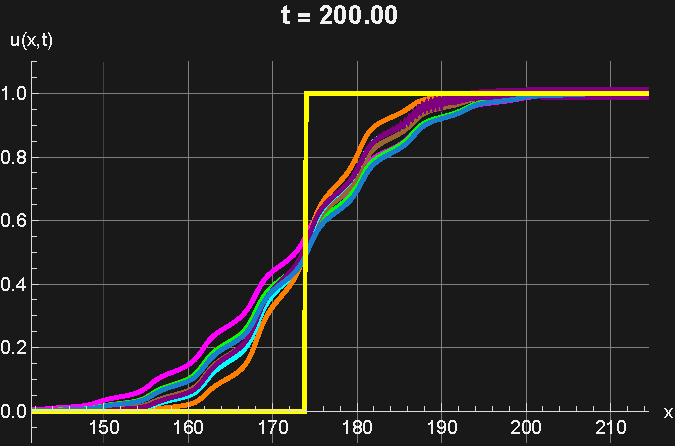
\includegraphics[height=5cm, keepaspectratio]{a_x_nejavn_t_200.pdf}
		\caption{Момент времени t=200}
	\end{subfigure}
	\hspace{0.05\textwidth}
	\begin{subfigure}[b]{0.45\textwidth}
		\centering
		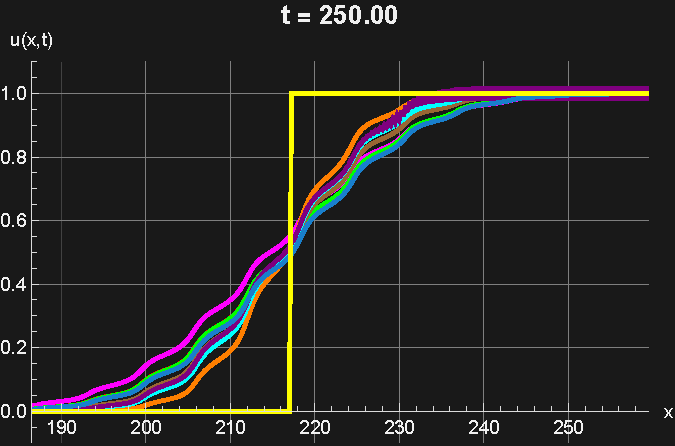
\includegraphics[height=5cm, keepaspectratio]{a_x_nejavn_t_250.pdf}
		\caption{Момент времени t=250}
	\end{subfigure}
	
	\caption{Сравнение аппроксимаций для всех схем при $a=a(x)$}
	\label{fig:all_schemes_nejavn_a_x}
\end{figure}

По данным, приведенным в таблице \ref{tab:norms_compact6}, можно сказать, что поведение норм ошибок для коэффициента, зависящего от пространства, сохраняет те же тенденции роста ошибки, что и для случая с постоянным коэффициентом переноса. Центральная схема вновь демонстрирует наибольшее значение ошибки, другие же схемы показывают сопоставимый уровень точности и схожий рост ошибки со временем. \\

\begin{table}[H]
	\centering
	\caption{Нормы ошибок для всех схем при $a=a(x)$}
	\label{tab:norms_compact6}
	\small
	\adjustbox{max width=\textwidth}{
		\begin{tabular}{|c|c|*{10}{c|}}
			\hline
			\rotatebox{90}{Норма} & $t$
			& \rotatebox{90}{Против потока }
			& \rotatebox{90}{Центральная }
			& \rotatebox{90}{ЛВ}
			& \rotatebox{90}{КН}
			& \rotatebox{90}{Общая пртв птк}
			& \rotatebox{90}{Лин. вязкость}
			& \rotatebox{90}{Вяз. 4-го поряд. }
			& \rotatebox{90}{Нелин. вязкость}
			& \rotatebox{90}{Годунов } \\
			\hline
			
			\multirow{6}{*}{$L_1$}
			& 10  & 2.067 & 10.821 & 2.354 & 1.276 & 2.055 & 2.259 & 3.344 & 2.221 & 2.327 \\
			& 20  & 2.700 & 19.836 & 3.088 & 1.540 & 2.680 & 2.692 & 3.686 & 2.685 & 2.927 \\
			& 100 & 6.296 & 91.924 & 6.995 & 3.909 & 6.256 & 5.763 & 6.510 & 6.454 & 6.513 \\
			& 150 & 7.724 & 135.543 & 8.577 & 4.807 & 7.676 & 6.971 & 7.614 & 8.140 & 7.936 \\
			& 200 & 8.941 & 173.577 & 9.933 & 5.584 & 8.885 & 8.004 & 8.562 & 8.883 & 9.145 \\
			& 250 & 10.028 & 216.695 & 11.165 & 6.303 & 9.967 & 8.936 & 9.423 & 8.790 & 10.218 \\
			\hline
			
			\multirow{6}{*}{$L_2$}
			& 10  & 0.790 & 2.890 & 0.838 & 0.608 & 0.788 & 0.836 & 1.137 & 0.839 & 0.942 \\
			& 20  & 0.849 & 4.090 & 0.913 & 0.627 & 0.846 & 0.853 & 1.136 & 0.827 & 0.979 \\
			& 100 & 1.347 & 9.214 & 1.424 & 1.048 & 1.343 & 1.291 & 1.467 & 1.251 & 1.433 \\
			& 150 & 1.494 & 11.303 & 1.584 & 1.166 & 1.490 & 1.422 & 1.574 & 1.381 & 1.572 \\
			& 200 & 1.612 & 13.055 & 1.714 & 1.266 & 1.607 & 1.529 & 1.665 & 1.483 & 1.683 \\
			& 250 & 1.716 & 14.613 & 1.833 & 1.361 & 1.711 & 1.626 & 1.749 & 1.566 & 1.780 \\
			\hline
			
			\multirow{6}{*}{$L_\infty$}
			& 10  & 0.510 & 1.000 & 0.520 & 0.493 & 0.510 & 0.586 & 0.865 & 0.545 & 1.000 \\
			& 20  & 0.520 & 1.000 & 0.535 & 0.515 & 0.520 & 0.586 & 0.865 & 0.546 & 1.000 \\
			& 100 & 0.511 & 1.000 & 0.540 & 0.510 & 0.511 & 0.586 & 0.865 & 0.531 & 1.000 \\
			& 150 & 0.504 & 1.000 & 0.539 & 0.500 & 0.504 & 0.586 & 0.865 & 0.531 & 1.000 \\
			& 200 & 0.499 & 1.480 & 0.540 & 0.493 & 0.499 & 0.586 & 0.865 & 0.531 & 1.000 \\
			& 250 & 0.504 & 1.506 & 0.549 & 0.502 & 0.504 & 0.586 & 0.865 & 0.531 & 1.000 \\
			\hline
	\end{tabular}}
\end{table}

Влияние коэффициента $a=a(x)$ проявляется преимущественно в количественном изменении норм, не меняя общей картины аппроксимации численного решения.

\begin{figure}[H]
	\vspace{10pt}
	\centering
	% Первая строка
	\begin{subfigure}[b]{0.45\textwidth}
		\centering
		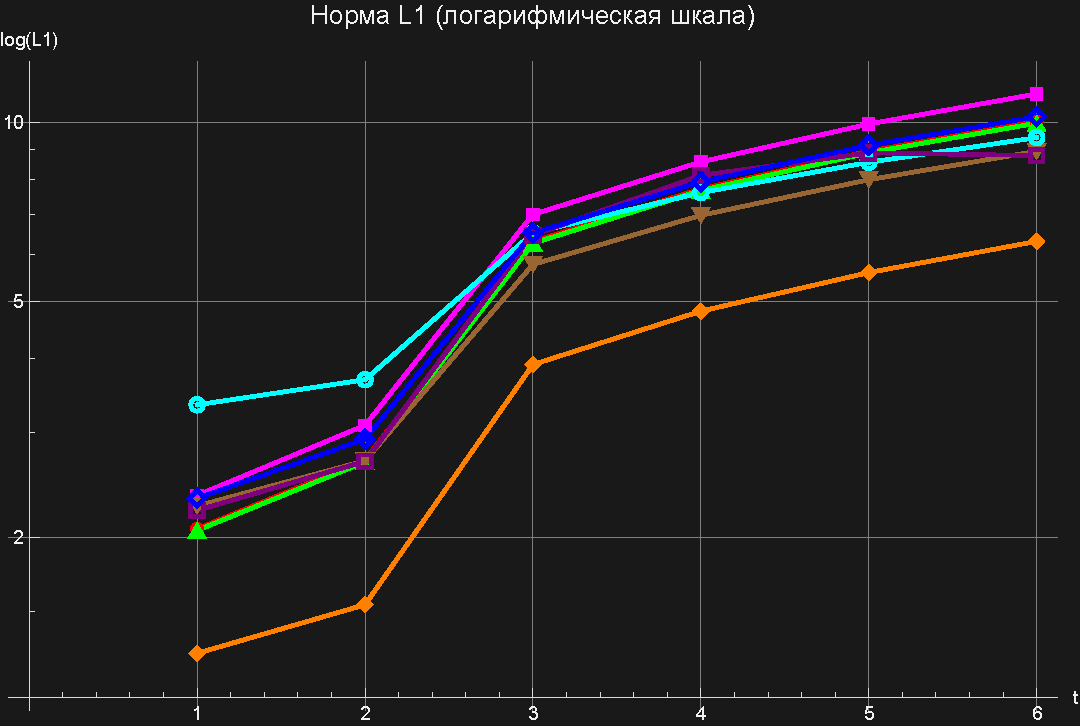
\includegraphics[height=5cm, keepaspectratio]{a_x_log_err_l1_nej.pdf}
		\caption{Логарифмический график ошибок для нормы $L_1$}
	\end{subfigure}
	\hspace{0.05\textwidth}
	\begin{subfigure}[b]{0.45\textwidth}
		\centering
		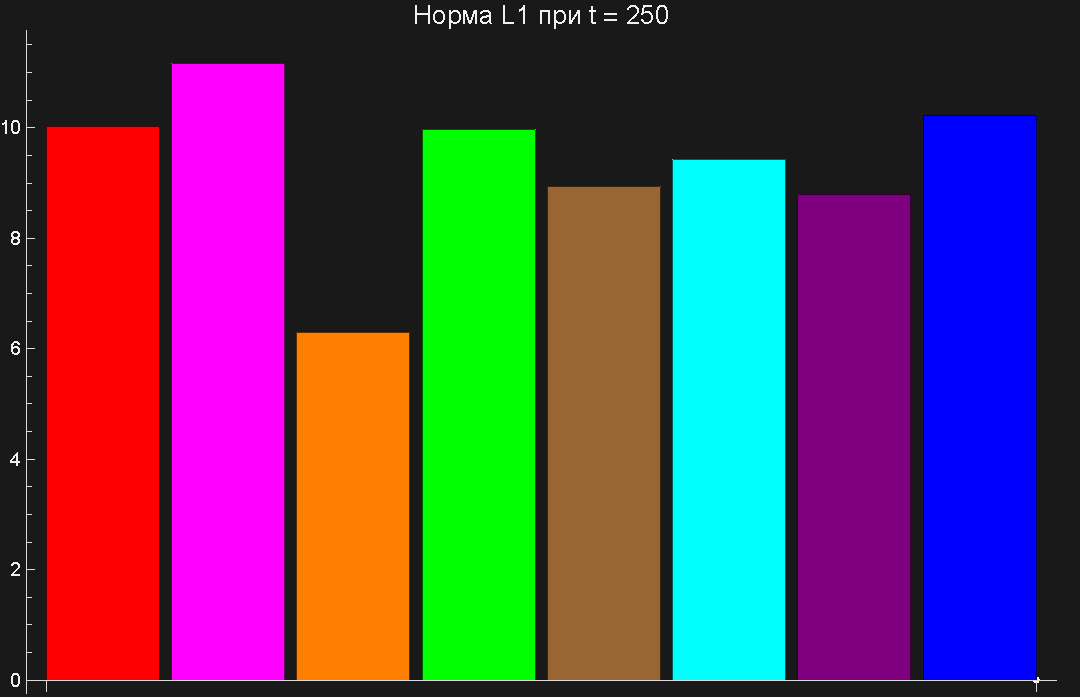
\includegraphics[height=5cm, keepaspectratio]{a_x_bar_err_l1_nej.pdf}
		\caption{Столбчатая диаграмма ошибки для нормы $L_1$ при t=250}
	\end{subfigure}
	
	\vspace{0.5cm}
	
	% Вторая строка
	\begin{subfigure}[b]{0.45\textwidth}
		\centering
		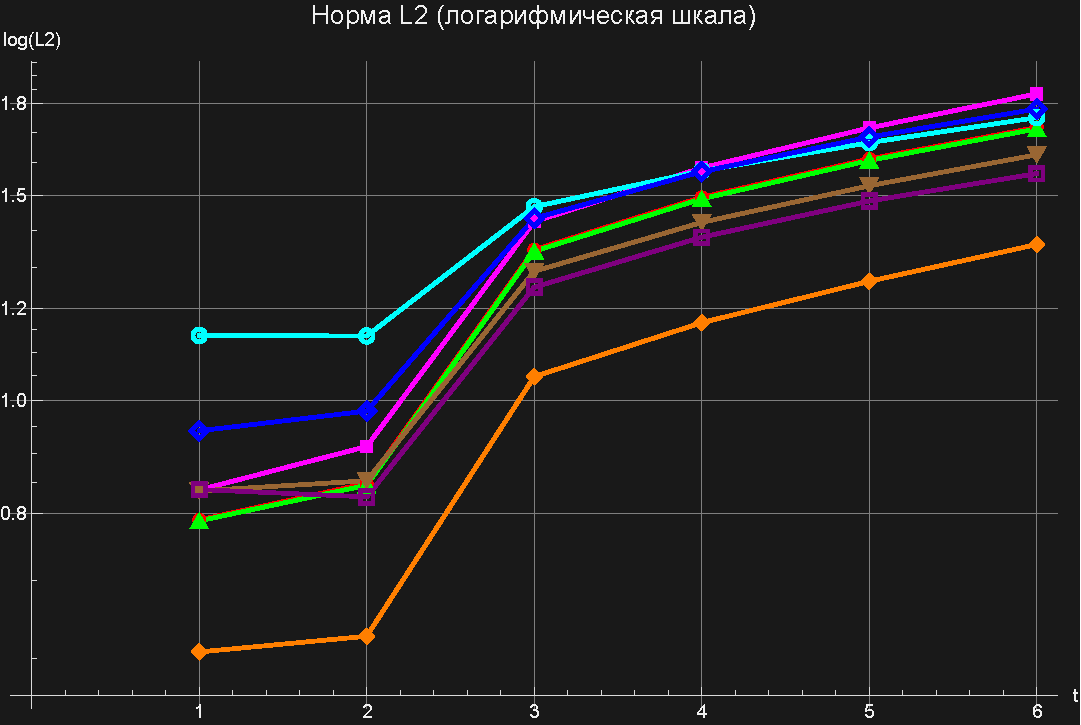
\includegraphics[height=5cm, keepaspectratio]{a_x_log_err_l2_nej.pdf}
		\caption{Логарифмический график ошибок для нормы $L_2$}
	\end{subfigure}
	\hspace{0.05\textwidth}
	\begin{subfigure}[b]{0.45\textwidth}
		\centering
		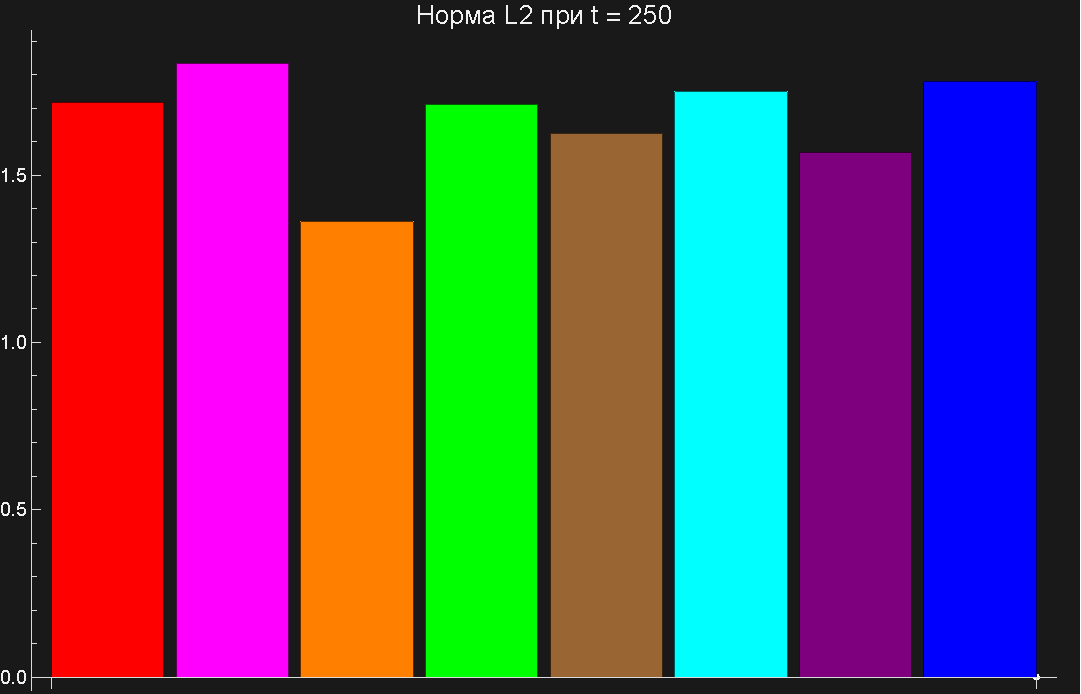
\includegraphics[height=5cm, keepaspectratio]{a_x_bar_err_l2_nej.pdf}
		\caption{Столбчатая диаграмма ошибки для нормы $L_2$ при t=250}
	\end{subfigure}
	
	\vspace{0.5cm}
	
	% Третья строка
	\begin{subfigure}[b]{0.45\textwidth}
		\centering
		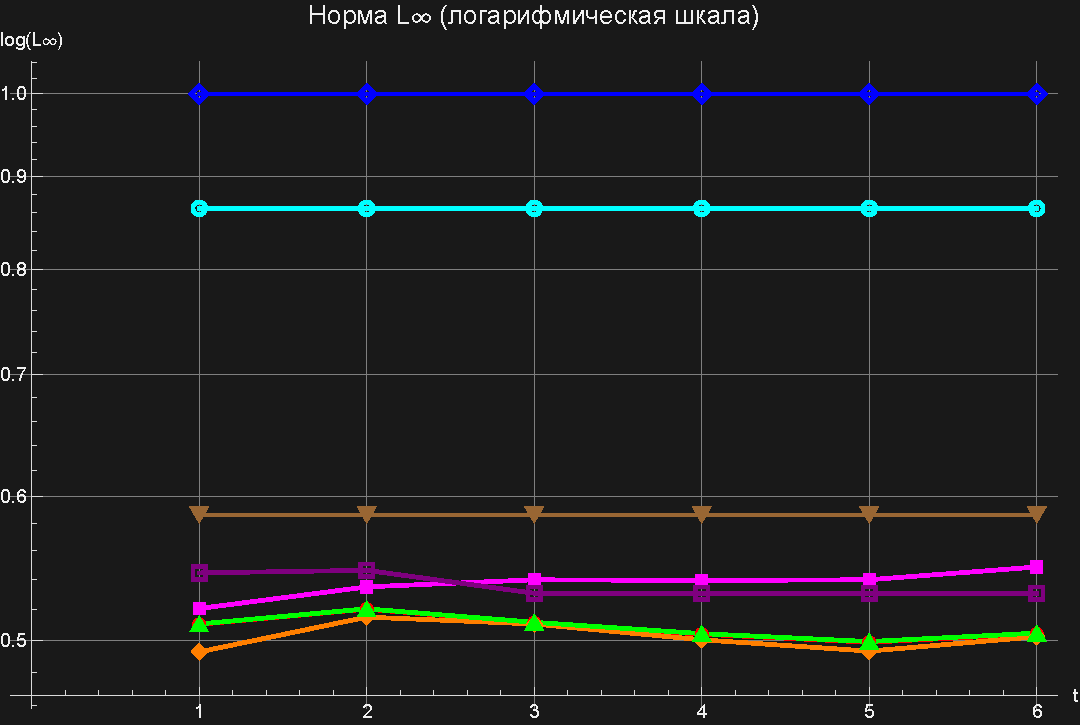
\includegraphics[height=5cm, keepaspectratio]{a_x_log_err_linf_nej.pdf}
		\caption{Логарифмический график ошибок для нормы $L_\infty$}
	\end{subfigure}
	\hspace{0.05\textwidth}
	\begin{subfigure}[b]{0.45\textwidth}
		\centering
		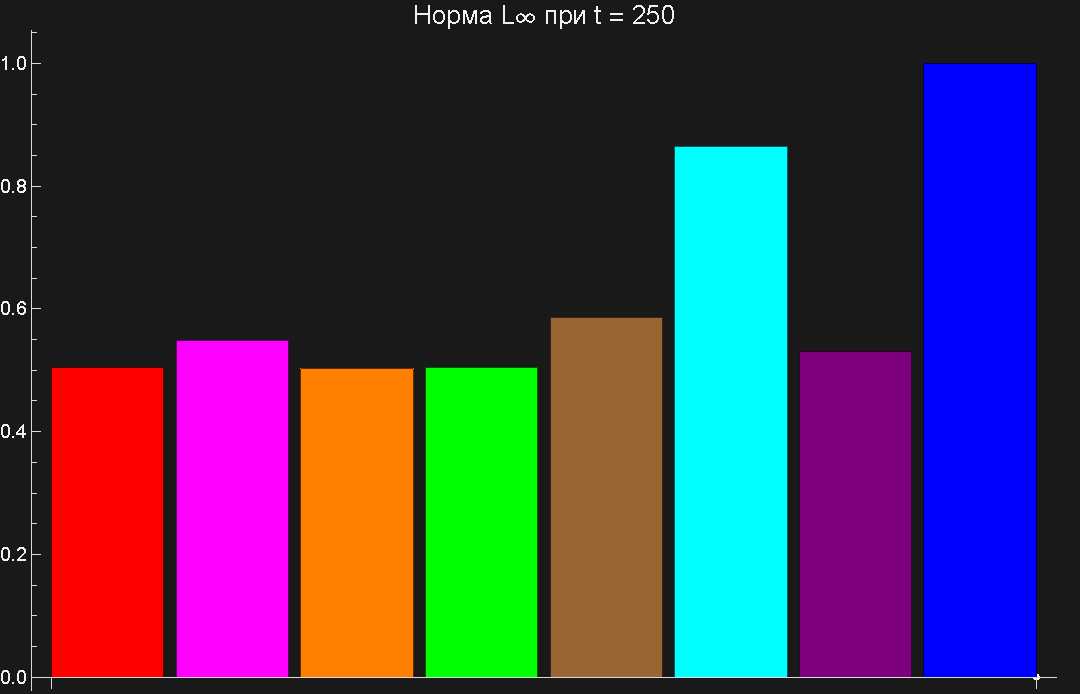
\includegraphics[height=5cm, keepaspectratio]{a_x_bar_err_linf_nej.pdf}
		\caption{Столбчатая диаграмма ошибки для нормы $L_\infty$ при t=250}
	\end{subfigure}
	
	\caption{Сравнение ошибок норм при  $a=a(x)$}
\end{figure}  

\section*{{Случай коэффициента, зависящего от времени $(a=a(t))$}}

Параметры аппроксимации:
\[
\begin{aligned}
	a(t) &= (-1)^{\lfloor t \rfloor}. \\
	h &= 0.025, \\
	\tau &= 0.05, \\
	x &\in [-10,\,10], \\
	N &= 1000.
\end{aligned}
\]

Параметры выбраны таким образом, чтобы показать преимущества неявных схем, при данных параметрах, численное решение явных схем просто взорвалось бы.

Поведение решения в случая коэффициента, зависящего от времени ($a=a(t)$), имеет те же принципиальные особенности, что и описанные выше для явынх схем. Несмотря на то, что неявные схемы обладают большим преимуществом, которое допускает более крупные шаги по пространственно-временной сетке, они также строятся как пошаговая эволюция решения вперед по времени и не способны аппроксимировать движение вдоль одной и той же характеристики в обратном направлении по времени.

Вследствие этого при периодической смене знака коэффициента скорости наблюдается аналогичное накопление численной диссипации при каждом возврате профиля в исходную область по пространственной координате. Отличие неявных схем проявляется преимущественно в степени сглаживания решения: диссипативные свойства выражены сильнее, однако качественная картина процесса и интерпретация расхождения с аналитическим решением полностью совпадают со случаем численного решения явных схем.

\begin{figure}[H]
	\vspace{10pt}
	\centering
	% Первая строка
	\begin{subfigure}[b]{0.45\textwidth}
		\centering
		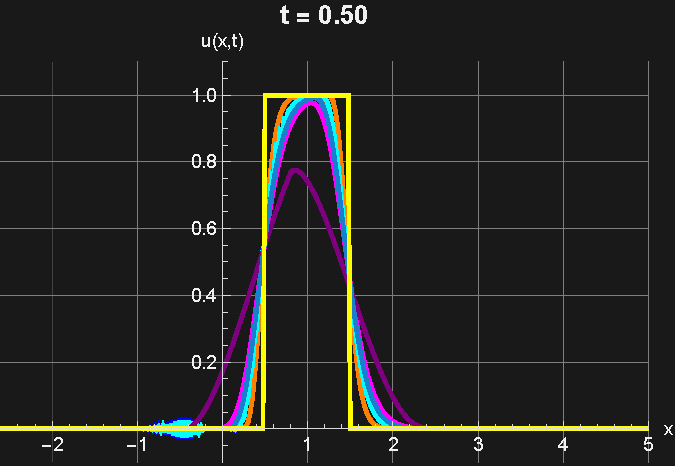
\includegraphics[height=5cm, keepaspectratio]{a_t_nejavn_t_0_50.pdf}
		\caption{Момент времени t=0.5}
	\end{subfigure}
	\hspace{0.05\textwidth}
	\begin{subfigure}[b]{0.45\textwidth}
		\centering
		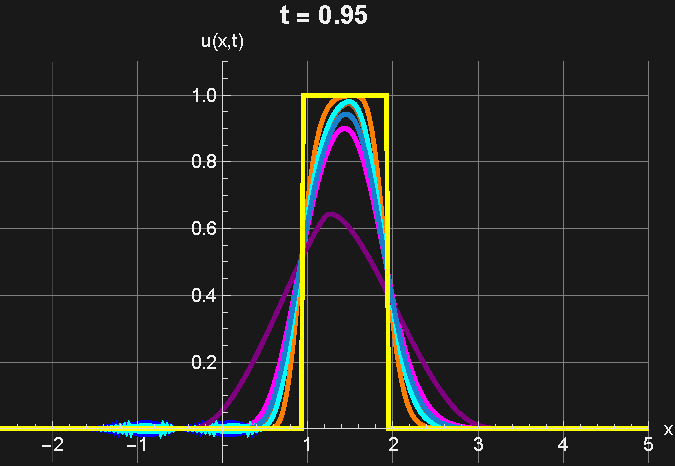
\includegraphics[height=5cm, keepaspectratio]{a_t_nejavn_t_0_95.pdf}
		\caption{Момент времени t=0.95}
	\end{subfigure}
	
	\vspace{0.5cm}
	
	% Вторая строка
	\begin{subfigure}[b]{0.45\textwidth}
		\centering
		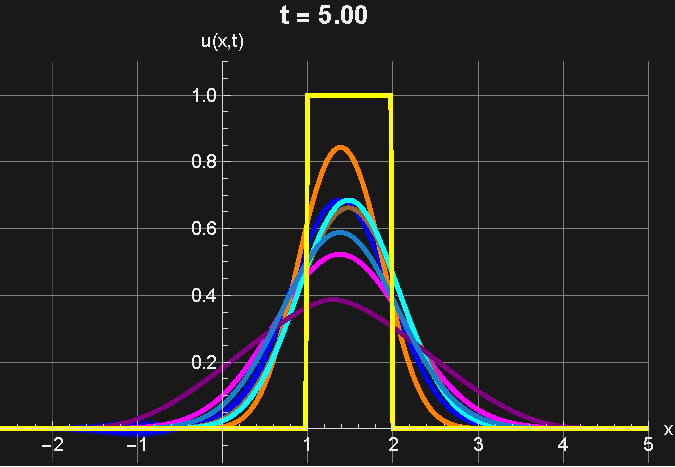
\includegraphics[height=5cm, keepaspectratio]{a_t_nejavn_t_5.pdf}
		\caption{Момент времени t=5}
	\end{subfigure}
	\hspace{0.05\textwidth}
	\begin{subfigure}[b]{0.45\textwidth}
		\centering
		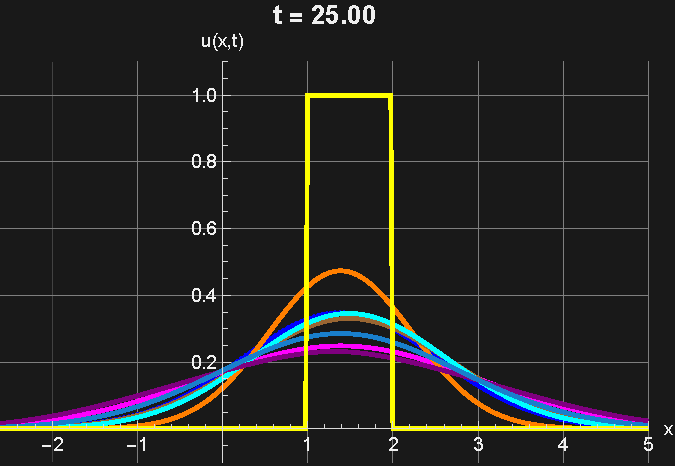
\includegraphics[height=5cm, keepaspectratio]{a_t_nejavn_t_25.pdf}
		\caption{Момент времени t=25}
	\end{subfigure}
	
	\vspace{0.5cm}
	
	% Третья строка
	\begin{subfigure}[b]{0.45\textwidth}
		\centering
		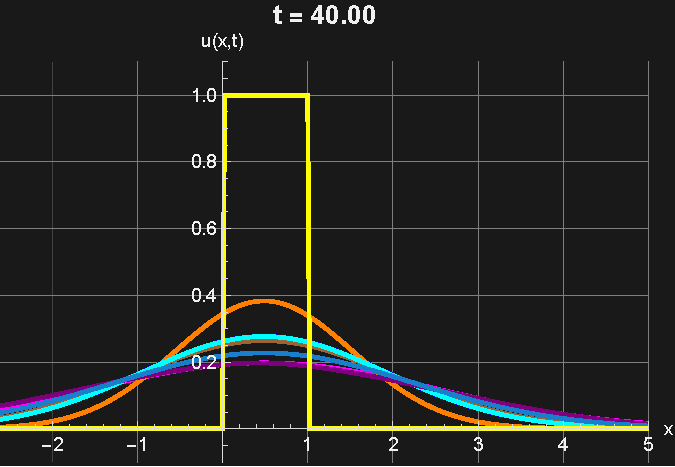
\includegraphics[height=5cm, keepaspectratio]{a_t_nejavn_t_40.pdf}
		\caption{Момент времени t=40}
	\end{subfigure}
	\hspace{0.05\textwidth}
	\begin{subfigure}[b]{0.45\textwidth}
		\centering
		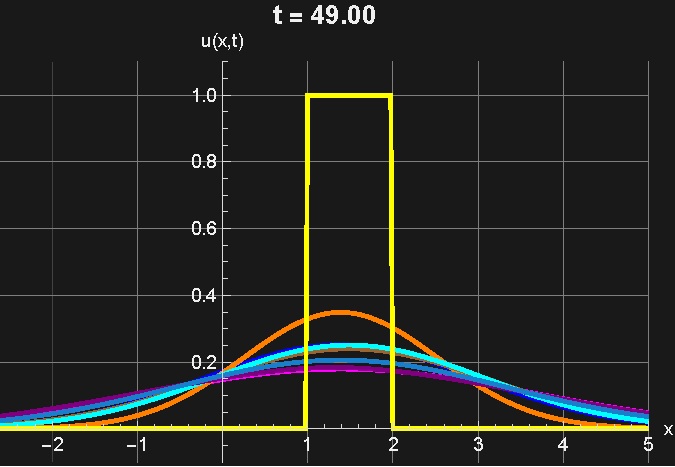
\includegraphics[height=5cm, keepaspectratio]{a_t_nejavn_t_49.pdf}
		\caption{Момент времени t=49}
	\end{subfigure}
	
	\caption{Сравнение аппроксимаций для всех схем при $a=a(t)$}
	\label{fig:all_schemes_nejavn_a_t}
\end{figure}

Таблица \ref{tab:norms_compact7} подтверждает, что при $a=a(t)$ рост ошибки, как и во всех вышеописанных случаях численного решения неявными разностными схемами, обусловлен накоплением численной диссипации при переодической смене направления переноса. 

\begin{table}[H]
	\centering
	\caption{Нормы ошибок для всех схем при $a=a(t)$}
	\label{tab:norms_compact7}
	\small
	\adjustbox{max width=\textwidth}{
		\begin{tabular}{|c|c|*{10}{c|}}
			\hline
			\rotatebox{90}{Норма} & $t$
			& \rotatebox{90}{Против потока }
			& \rotatebox{90}{Центральная }
			& \rotatebox{90}{ЛВ}
			& \rotatebox{90}{КН}
			& \rotatebox{90}{Общая пртв птк}
			& \rotatebox{90}{Лин. вязкость}
			& \rotatebox{90}{Вяз. 4-го поряд. }
			& \rotatebox{90}{Нелин. вязкость}
			& \rotatebox{90}{Годунов } \\
			\hline
			
			\multirow{6}{*}{$L_1$}
			& 0.5  & 0.306 & 0.264 & 0.353 & 0.176 & 0.306 & 0.262 & 0.260 & 0.689 & 0.306 \\
			& 0.95 & 0.424 & 0.370 & 0.489 & 0.244 & 0.424 & 0.363 & 0.360 & 0.875 & 0.424 \\
			& 5    & 0.932 & 0.801 & 1.033 & 0.585 & 0.932 & 0.811 & 0.778 & 1.275 & 0.932 \\
			& 25   & 1.443 & 1.332 & 1.512 & 1.111 & 1.443 & 1.357 & 1.329 & 1.548 & 1.443 \\
			& 40   & 1.551 & 1.458 & 1.609 & 1.262 & 1.551 & 1.481 & 1.458 & 1.611 & 1.551 \\
			& 49   & 1.593 & 1.507 & 1.646 & 1.326 & 1.593 & 1.528 & 1.507 & 1.638 & 1.593 \\
			\hline
			
			\multirow{6}{*}{$L_2$}
			& 0.5  & 0.301 & 0.275 & 0.323 & 0.228 & 0.301 & 0.279 & 0.274 & 0.487 & 0.301 \\
			& 0.95 & 0.355 & 0.320 & 0.383 & 0.268 & 0.355 & 0.328 & 0.320 & 0.570 & 0.355 \\
			& 5    & 0.590 & 0.529 & 0.634 & 0.442 & 0.590 & 0.530 & 0.515 & 0.740 & 0.590 \\
			& 25   & 0.803 & 0.759 & 0.829 & 0.668 & 0.803 & 0.769 & 0.758 & 0.843 & 0.803 \\
			& 40   & 0.844 & 0.808 & 0.865 & 0.730 & 0.844 & 0.817 & 0.808 & 0.866 & 0.844 \\
			& 49   & 0.860 & 0.828 & 0.879 & 0.757 & 0.860 & 0.835 & 0.827 & 0.876 & 0.860 \\
			\hline
			
			\multirow{6}{*}{$L_\infty$}
			& 0.5  & 0.517 & 0.546 & 0.517 & 0.500 & 0.517 & 0.517 & 0.538 & 0.560 & 0.517 \\
			& 0.95 & 0.514 & 0.512 & 0.515 & 0.500 & 0.514 & 0.512 & 0.512 & 0.587 & 0.514 \\
			& 5    & 0.599 & 0.589 & 0.614 & 0.602 & 0.599 & 0.525 & 0.519 & 0.691 & 0.599 \\
			& 25   & 0.739 & 0.696 & 0.768 & 0.629 & 0.739 & 0.695 & 0.684 & 0.787 & 0.739 \\
			& 40   & 0.782 & 0.741 & 0.809 & 0.660 & 0.782 & 0.751 & 0.740 & 0.812 & 0.782 \\
			& 49   & 0.803 & 0.765 & 0.827 & 0.694 & 0.803 & 0.771 & 0.761 & 0.826 & 0.803 \\
			\hline
			
	\end{tabular}}
\end{table}

Следует подчеркнуть, что значения норм не свидетельствуют о потере корректности разностных схем. Возврат профиля назад в пространстве при изменении знака коэффициента скокрости переноса, не сопровождается аналогичным возвратом назад по времени. Таким образом полученные графические результаты, ошибка норм и аналитическое решение данного случая коэффициента переноса по характеристикам полностью согласуются и отражают фундаментальные ограничения разностных схем при моделировании возвратно-поступательного движения. 

\begin{figure}[H]
	\vspace{10pt}
	\centering
	% Первая строка
	\begin{subfigure}[b]{0.45\textwidth}
		\centering
		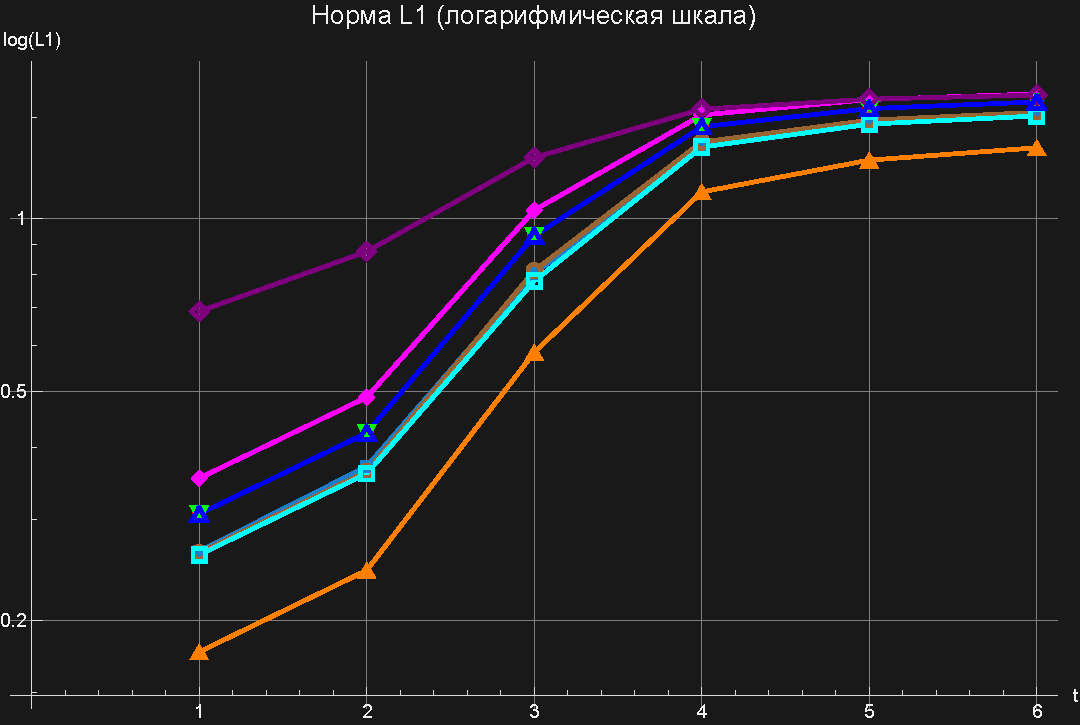
\includegraphics[height=5cm, keepaspectratio]{a_t_log_err_l1_nej.pdf}
		\caption{Логарифмический график ошибок для нормы $L_1$}
	\end{subfigure}
	\hspace{0.05\textwidth}
	\begin{subfigure}[b]{0.45\textwidth}
		\centering
		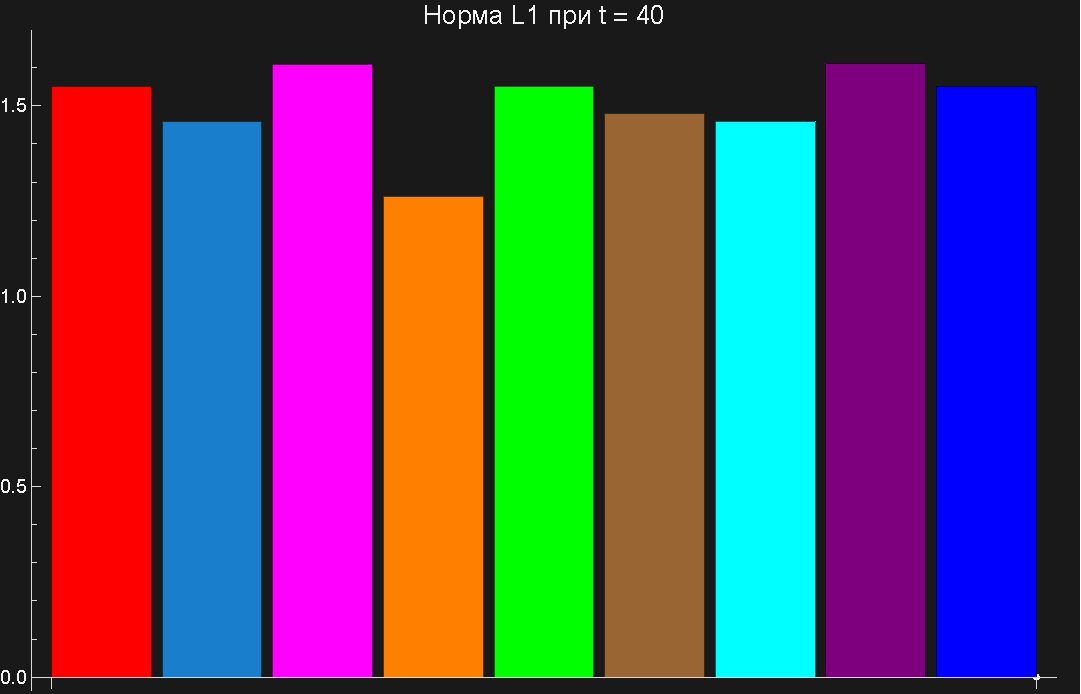
\includegraphics[height=5cm, keepaspectratio]{a_t_bar_err_l1_nej.pdf}
		\caption{Столбчатая диаграмма ошибки для нормы $L_1$ при t=250}
	\end{subfigure}
	
	\vspace{0.5cm}
	
	% Вторая строка
	\begin{subfigure}[b]{0.45\textwidth}
		\centering
		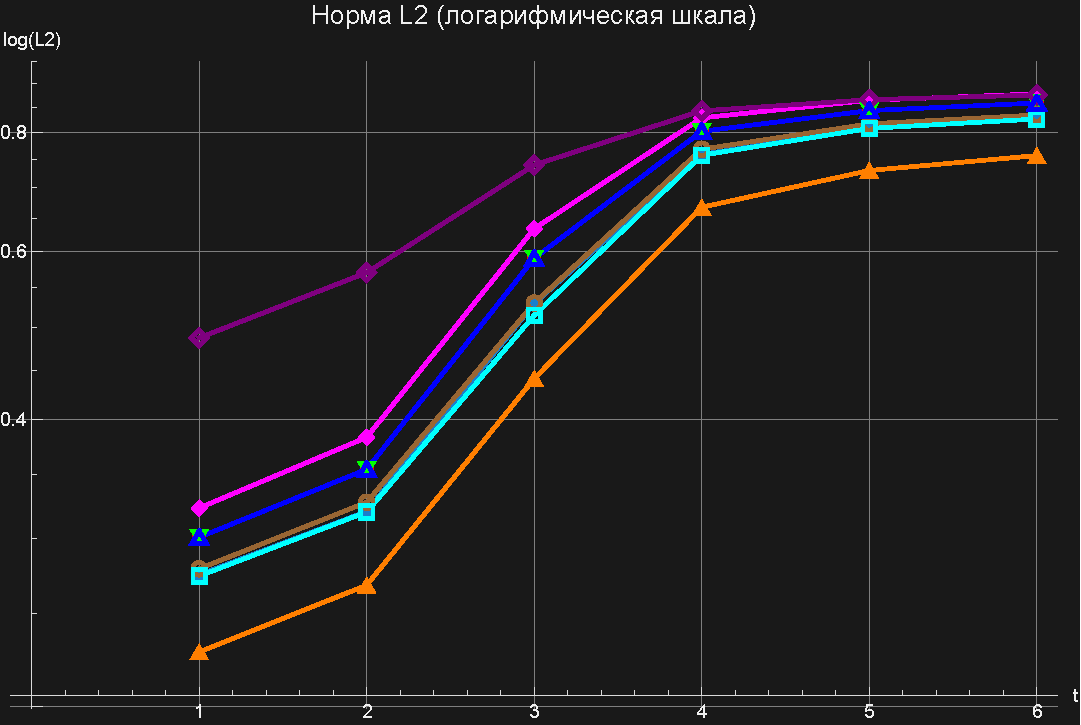
\includegraphics[height=5cm, keepaspectratio]{a_t_log_err_l2_nej.pdf}
		\caption{Логарифмический график ошибок для нормы $L_2$}
	\end{subfigure}
	\hspace{0.05\textwidth}
	\begin{subfigure}[b]{0.45\textwidth}
		\centering
		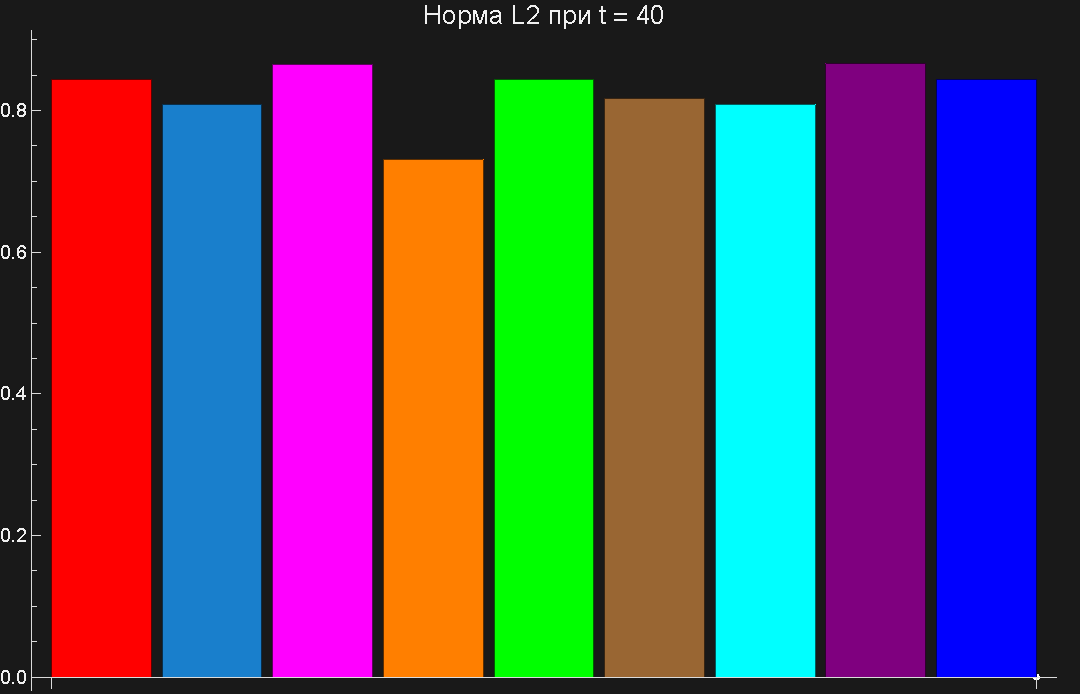
\includegraphics[height=5cm, keepaspectratio]{a_t_bar_err_l2_nej.pdf}
		\caption{Столбчатая диаграмма ошибки для нормы $L_2$ при t=250}
	\end{subfigure}
	
	\vspace{0.5cm}
	
	% Третья строка
	\begin{subfigure}[b]{0.45\textwidth}
		\centering
		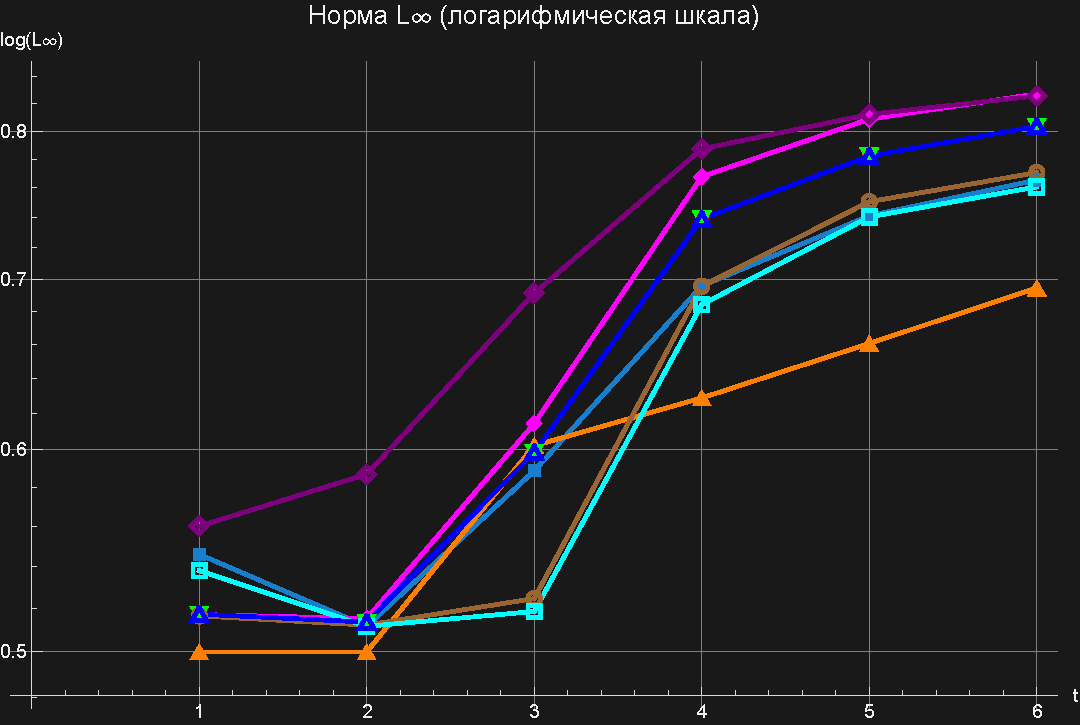
\includegraphics[height=5cm, keepaspectratio]{a_t_log_err_linf_nej.pdf}
		\caption{Логарифмический график ошибок для нормы $L_\infty$}
	\end{subfigure}
	\hspace{0.05\textwidth}
	\begin{subfigure}[b]{0.45\textwidth}
		\centering
		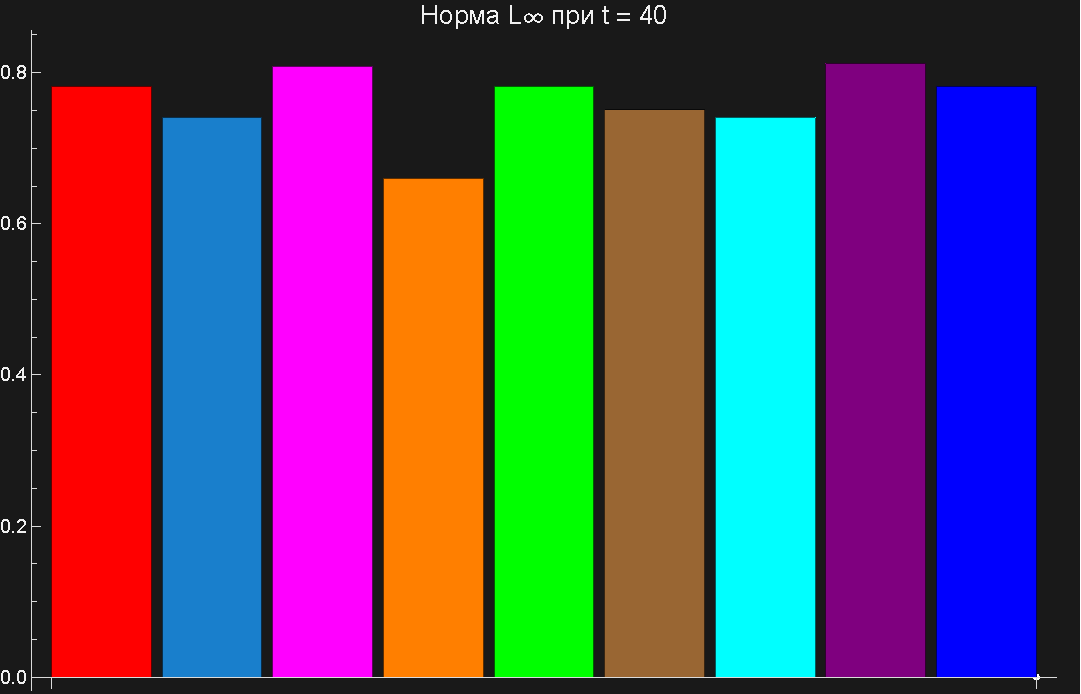
\includegraphics[height=5cm, keepaspectratio]{a_t_bar_err_linf_nej.pdf}
		\caption{Столбчатая диаграмма ошибки для нормы $L_\infty$ при t=250}
	\end{subfigure}
	
	\caption{Сравнение ошибок норм при  $a=a(t)$}
\end{figure}  

\section*{{Случай нестационарного коэффициента $(a(x,t)=x-t)$}}

Параметры аппроксимации:
\[
\begin{aligned}
	h &= 0.025, \\
	\tau &= 0.05, \\
	x &\in [-20,\,20], \\
	N &= 500.
\end{aligned}
\]

Для сравнения явных и неявных схем данный случай коэфициента преноса является очень показательным. Даже при задании параметров аппроксимации видно, что для явного случая параметры тщательно подбирались, то есть не любой шаг по пространственно -- временной сетке мог подойти, иначе решения могло просто численно взорваться. В неявном случая же в таких расчетах нет нужды, расчёты остаются стабильными при значительно более широком диапазоне параметров, и необходимость детальной проверки шагов отпадает.

Из рисунка \ref{fig_lbl:x_t_1} видно, что, несмотря на ослабленные требования к выбору параметров для неявной схемы, у некоторых методов всё же наблюдаются выраженные осцилляции. На этом рисунке -- это схемы "Неявная центральная схема","Схема с линейной вязкостью","Схема с линейной вязкостью 4-ого порядка", поэтому данные схемы были исключены из последующих графиков, чтобы не затруднять анализ более удачных методов аппроксимации.

\begin{figure}[H]
	\vspace{10pt}
	\centering
	% Первая строка
	\begin{subfigure}[b]{0.45\textwidth}
		\centering
		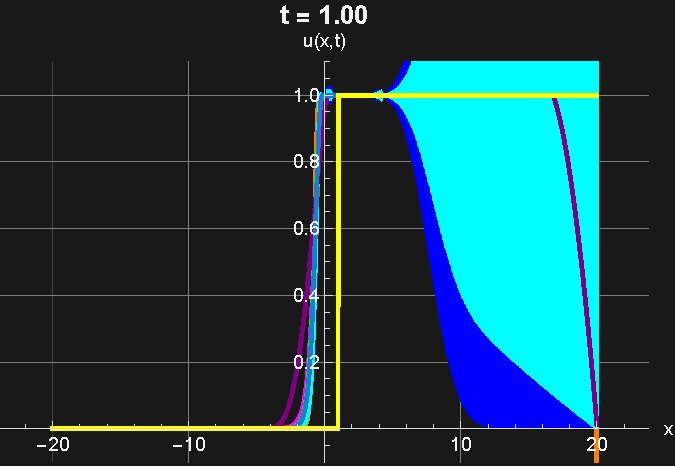
\includegraphics[height=5cm, keepaspectratio]{a_x_t_nejavn_t_1.pdf}
		\caption{Момент времени t=1}
		\label{fig_lbl:x_t_1}
	\end{subfigure}
	\hspace{0.05\textwidth}
	\begin{subfigure}[b]{0.45\textwidth}
		\centering
		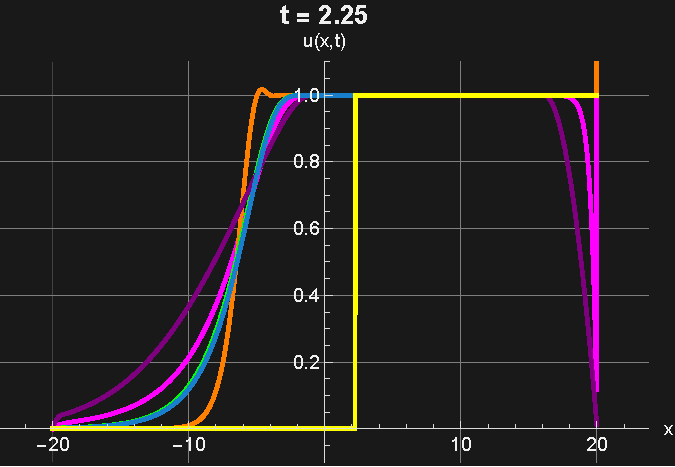
\includegraphics[height=5cm, keepaspectratio]{a_x_t_nejavn_t_2_25.pdf}
		\caption{Момент времени t=2.25}
	\end{subfigure}
	
	\vspace{0.5cm}
	
	% Вторая строка
	\begin{subfigure}[b]{0.45\textwidth}
		\centering
		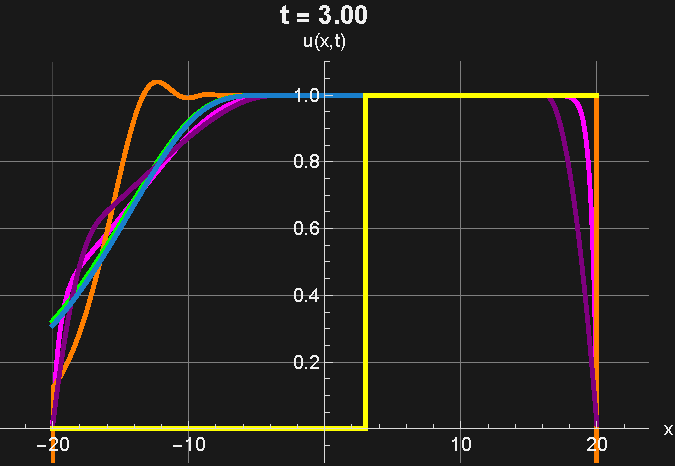
\includegraphics[height=5cm, keepaspectratio]{a_x_t_nejavn_t_3.pdf}
		\caption{Момент времени t=3}
	\end{subfigure}
	\hspace{0.05\textwidth}
	\begin{subfigure}[b]{0.45\textwidth}
		\centering
		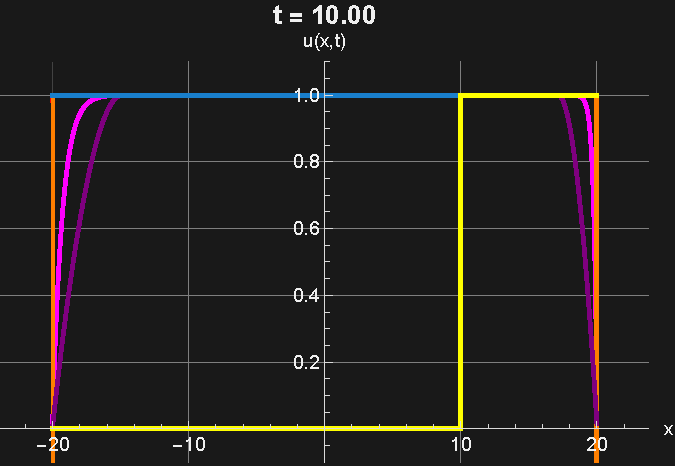
\includegraphics[height=5cm, keepaspectratio]{a_x_t_nejavn_t_10.pdf}
		\caption{Момент времени t=10}
	\end{subfigure}
	
	\vspace{0.5cm}
	
	% Третья строка
	\begin{subfigure}[b]{0.45\textwidth}
		\centering
		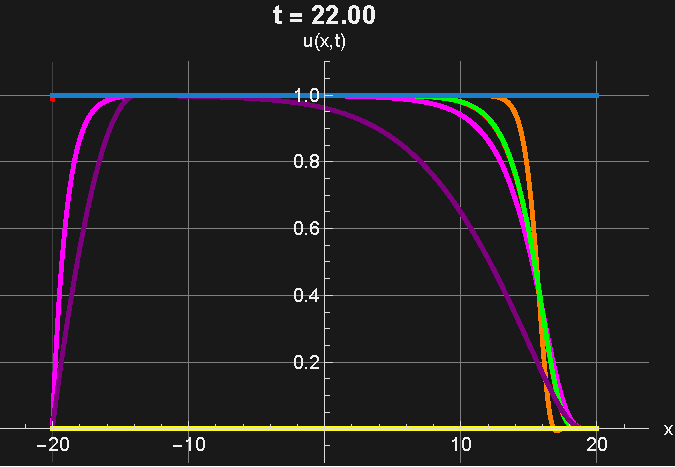
\includegraphics[height=5cm, keepaspectratio]{a_x_t_nejavn_t_22.pdf}
		\caption{Момент времени t=22}
	\end{subfigure}
	\hspace{0.05\textwidth}
	\begin{subfigure}[b]{0.45\textwidth}
		\centering
		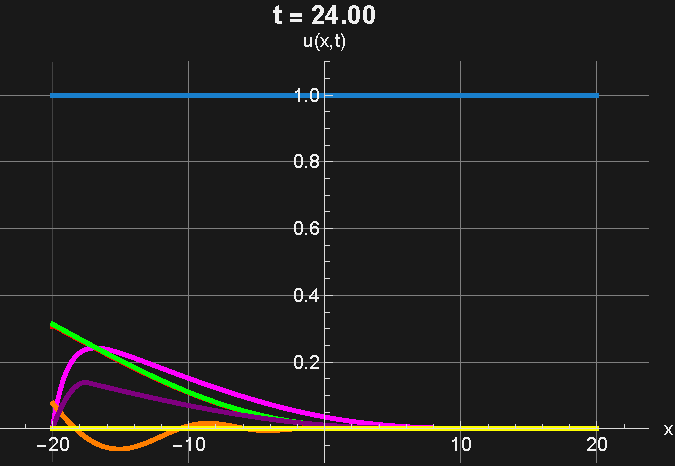
\includegraphics[height=5cm, keepaspectratio]{a_x_t_nejavn_t_24.pdf}
		\caption{Момент времени t=24}
	\end{subfigure}
	
	\caption{Сравнение аппроксимаций для всех схем при $a(x,t)=x-t$}
	\label{fig:all_schemes_nejavn_a_x_t}
\end{figure}

\begin{table}[H]
	\centering
	\caption{Нормы ошибок для всех схем при $a(x,t)=x-t$}
	\label{tab:norms_compact8}
	\small
	\adjustbox{max width=\textwidth}{
		\begin{tabular}{|c|c|*{10}{c|}}
			\hline
			\rotatebox{90}{Норма} & $t$
			& \rotatebox{90}{Против потока }
			& \rotatebox{90}{Центральная }
			& \rotatebox{90}{ЛВ}
			& \rotatebox{90}{КН}
			& \rotatebox{90}{Общая пртв птк}
			& \rotatebox{90}{Лин. вязкость}
			& \rotatebox{90}{Вяз. 4-го поряд. }
			& \rotatebox{90}{Нелин. вязкость}
			& \rotatebox{90}{Годунов } \\
			\hline
			
			\multirow{6}{*}{$L_1$}
			& 1    & 1.834 & 14.835 & 2.290 & 1.805 & 1.834 & 2.781 & 11.249 & 3.484 & 1.812 \\
			& 2.25 & 9.277 & 26.456 & 10.274 & 8.917 & 9.277 & 9.700 & 19.831 & 12.494 & 9.165 \\
			& 3    & 19.087 & 37.117 & 19.300 & 19.804 & 19.088 & 19.423 & 29.418 & 20.307 & 18.951 \\
			& 10   & 30.000 & 42.000 & 29.502 & 29.975 & 30.000 & 30.544 & 36.502 & 29.238 & 30.000 \\
			& 22   & 35.049 & 42.200 & 33.690 & 35.281 & 35.076 & 35.453 & 36.792 & 29.004 & 40.025 \\
			& 24   & 2.068 & 42.400 & 2.534 & 0.416 & 2.097 & 2.411 & 20.691 & 1.177 & 40.025 \\
			\hline
			
			\multirow{6}{*}{$L_2$}
			& 1    & 1.278 & 6.996 & 1.353 & 1.300 & 1.278 & 1.440 & 3.002 & 1.581 & 1.271 \\
			& 2.25 & 2.797 & 7.444 & 2.842 & 2.887 & 2.797 & 2.817 & 3.960 & 3.049 & 2.781 \\
			& 3    & 4.118 & 8.235 & 4.103 & 4.330 & 4.118 & 4.095 & 4.939 & 4.198 & 4.098 \\
			& 10   & 5.477 & 13.036 & 5.388 & 5.475 & 5.477 & 5.572 & 6.812 & 5.307 & 5.477 \\
			& 22   & 5.833 & 16.025 & 5.638 & 5.902 & 5.836 & 5.978 & 7.269 & 5.032 & 6.327 \\
			& 24   & 0.576 & 16.589 & 0.609 & 0.140 & 0.584 & 0.768 & 3.653 & 0.302 & 6.327 \\
			\hline
			
			\multirow{6}{*}{$L_\infty$}
			& 1    & 1.000 & 38.000 & 1.000 & 1.000 & 1.000 & 1.000 & 1.017 & 1.000 & 1.000 \\
			& 2.25 & 1.000 & 35.500 & 1.000 & 1.017 & 1.000 & 1.000 & 1.001 & 1.000 & 1.000 \\
			& 3    & 1.000 & 34.000 & 1.000 & 1.040 & 1.000 & 1.000 & 1.060 & 1.000 & 1.000 \\
			& 10   & 1.000 & 60.000 & 1.000 & 1.000 & 1.000 & 1.923 & 1.934 & 1.000 & 1.000 \\
			& 22   & 1.000 & 84.000 & 1.000 & 1.000 & 1.000 & 1.944 & 1.952 & 0.999 & 1.000 \\
			& 24   & 1.000 & 88.000 & 1.000 & 0.069 & 1.000 & 0.594 & 0.963 & 0.121 & 1.000 \\
			\hline
			
	\end{tabular}}
\end{table}

Из таблицы \ref{tab:norms_compact8} видно, что при коэффициенте переноса $a(x,t)=x-t$ поведение большинства схем носит согласованный характер. Значения норм $L_1$, $L_2$ и $L_\infty$ для устойчивых схем имеют сопоставимый порядок величин на протяжении всего интервала времени.

\begin{figure}[H]
	\vspace{10pt}
	\centering
	% Первая строка
	\begin{subfigure}[b]{0.45\textwidth}
		\centering
		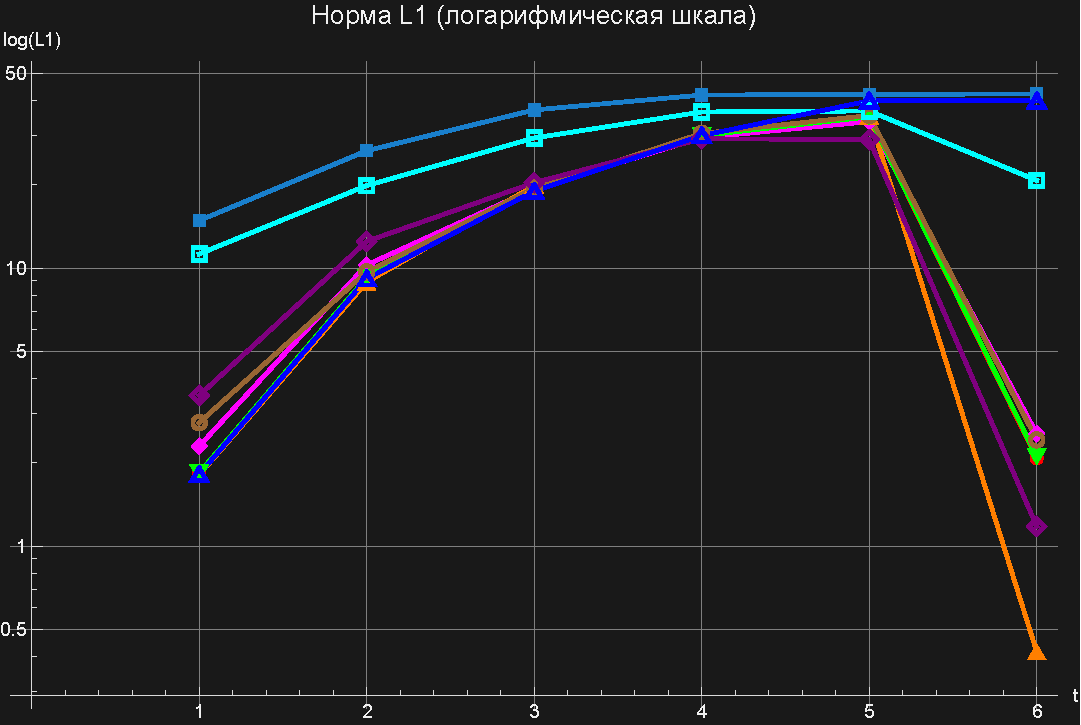
\includegraphics[height=5cm, keepaspectratio]{a_x_t_log_err_l1_nej.pdf}
		\caption{Логарифмический график ошибок для нормы $L_1$}
	\end{subfigure}
	\hspace{0.05\textwidth}
	\begin{subfigure}[b]{0.45\textwidth}
		\centering
		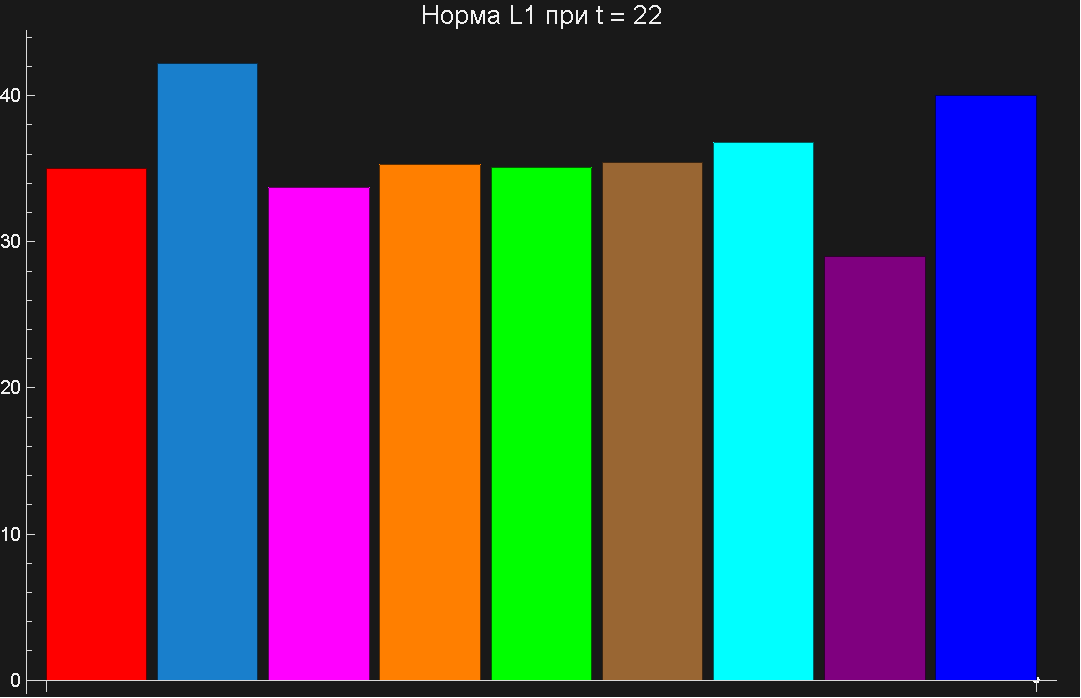
\includegraphics[height=5cm, keepaspectratio]{a_x_t_bar_err_l1_nej.pdf}
		\caption{Столбчатая диаграмма ошибки для нормы $L_1$ при t=22}
	\end{subfigure}
	
	\vspace{0.5cm}
	
	% Вторая строка
	\begin{subfigure}[b]{0.45\textwidth}
		\centering
		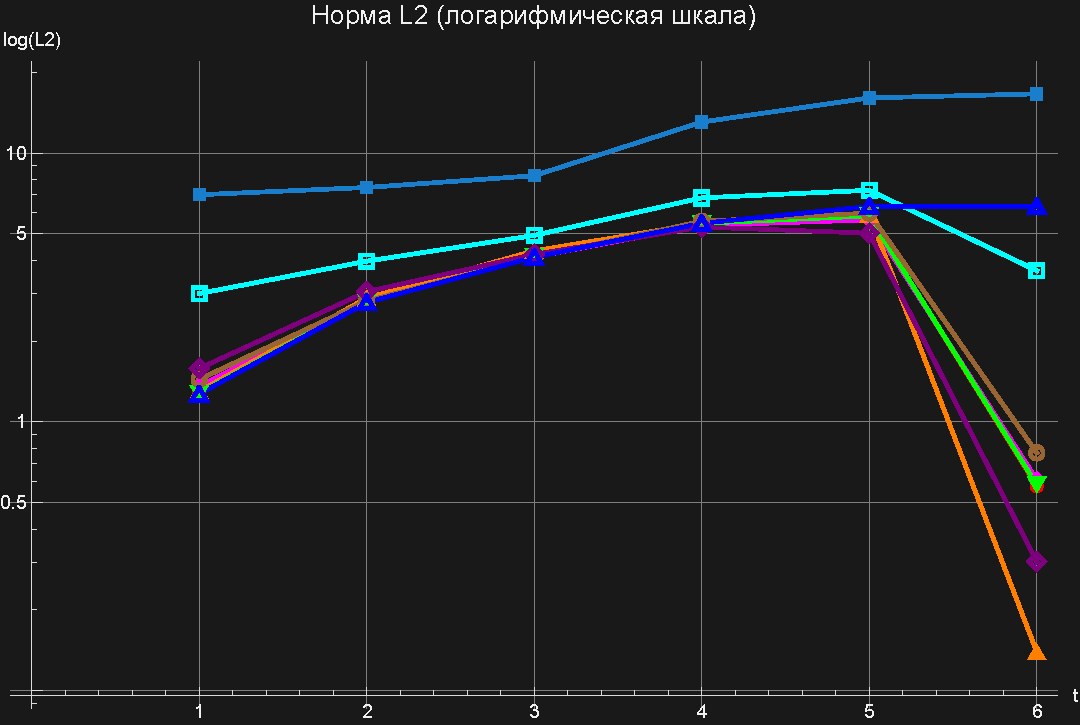
\includegraphics[height=5cm, keepaspectratio]{a_x_t_log_err_l2_nej.pdf}
		\caption{Логарифмический график ошибок для нормы $L_2$}
	\end{subfigure}
	\hspace{0.05\textwidth}
	\begin{subfigure}[b]{0.45\textwidth}
		\centering
		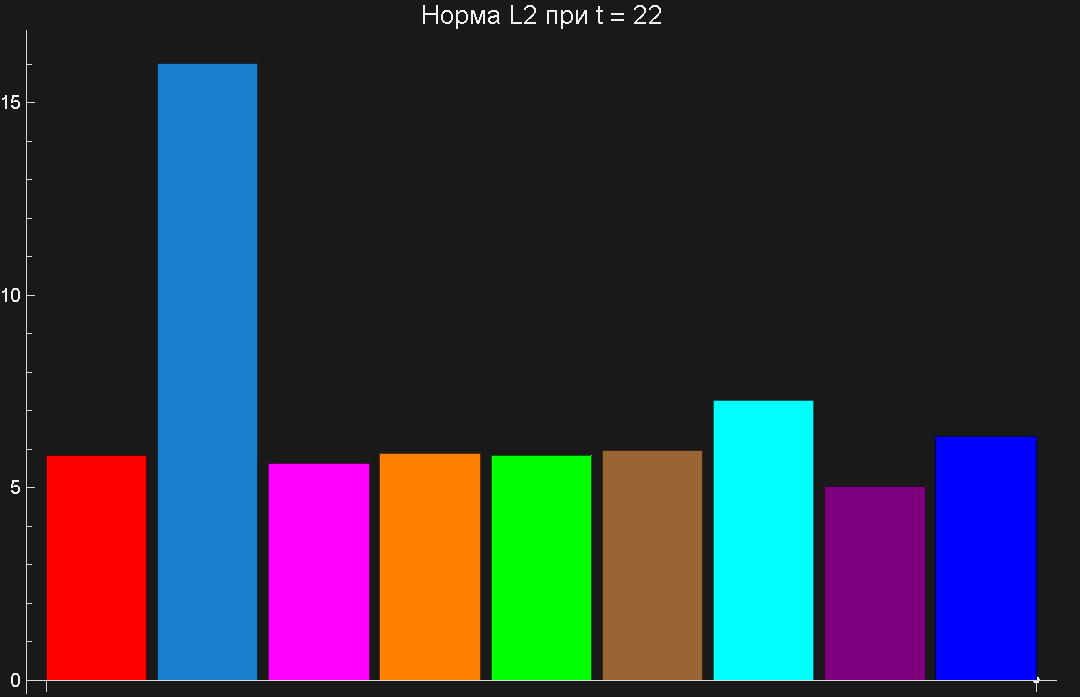
\includegraphics[height=5cm, keepaspectratio]{a_x_t_bar_err_l2_nej.pdf}
		\caption{Столбчатая диаграмма ошибки для нормы $L_2$ при t=22}
	\end{subfigure}
	
	\vspace{0.5cm}
	
	% Третья строка
	\begin{subfigure}[b]{0.45\textwidth}
		\centering
		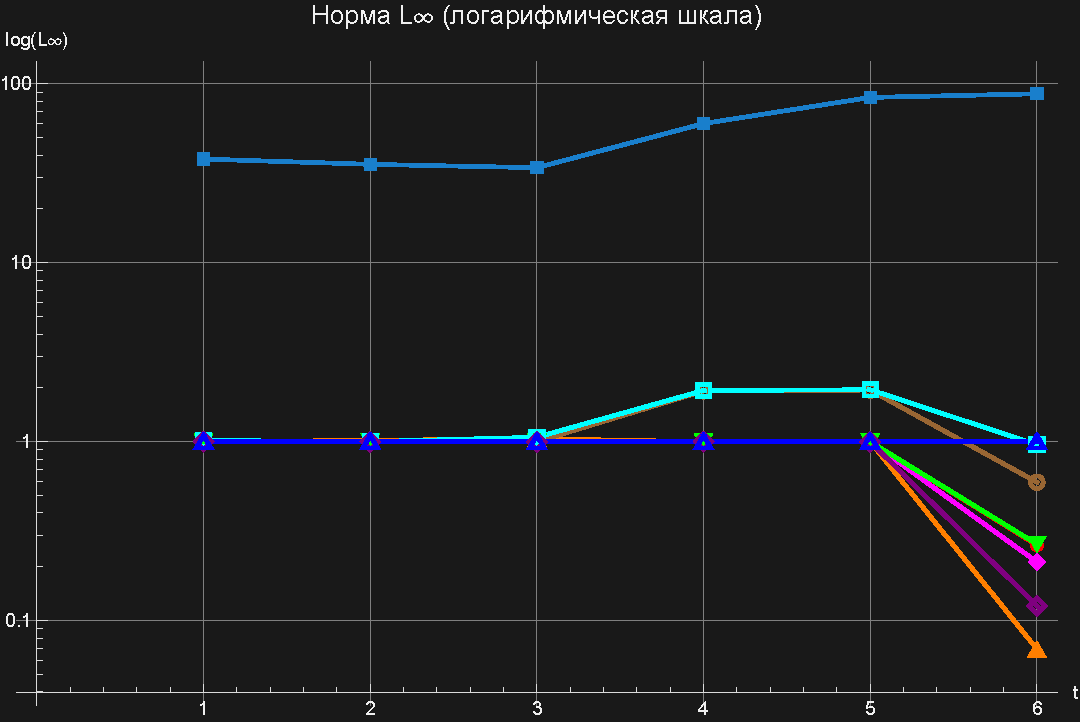
\includegraphics[height=5cm, keepaspectratio]{a_x_t_log_err_linf_nej.pdf}
		\caption{Логарифмический график ошибок для нормы $L_\infty$}
	\end{subfigure}
	\hspace{0.05\textwidth}
	\begin{subfigure}[b]{0.45\textwidth}
		\centering
		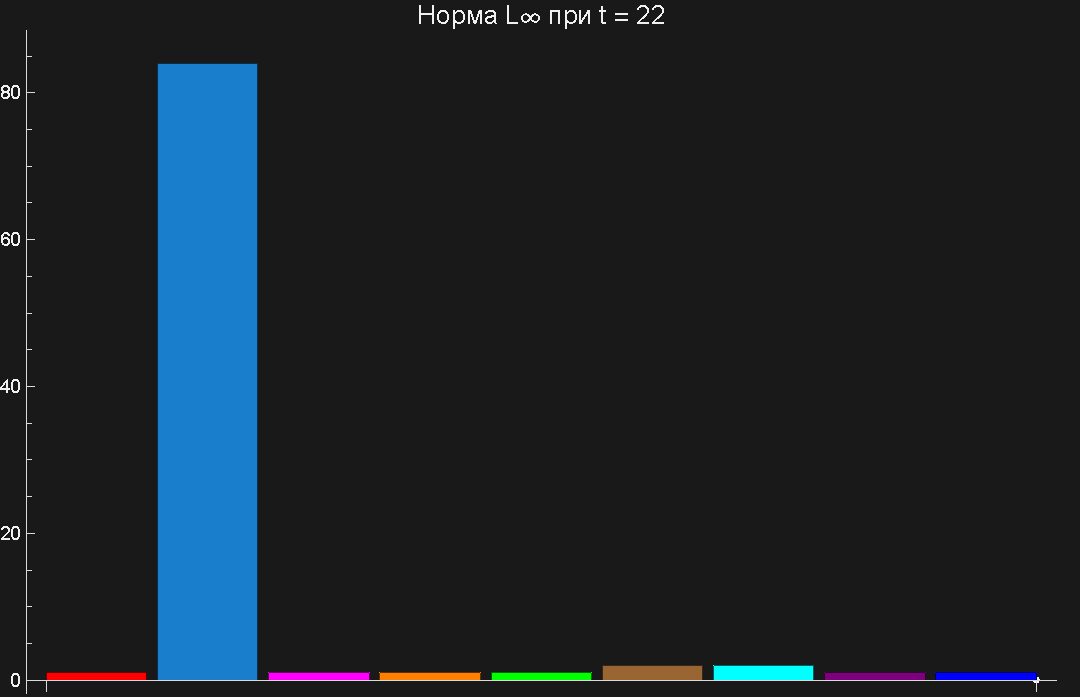
\includegraphics[height=5cm, keepaspectratio]{a_x_t_bar_err_linf_nej.pdf}
		\caption{Столбчатая диаграмма ошибки для нормы $L_\infty$ при t=22}
	\end{subfigure}
	
	\caption{Сравнение ошибок норм при  $a(x,t)=x-t$}
\end{figure} 

Схема Кранка--Николсона в данном случае не демонстрирует аномального роста 
ошибок и по значениям норм находится на уровне схем «против потока» и 
Лакса--Вендрофа. Это указывает на то, что при выбранных параметрах 
аппроксимации её диффузорные свойства не приводят к существенной 
деградации точности.

Следует отметить, что центральная схема существенно уступает остальным 
по всем нормам, что связано с развитием осцилляций при переменном 
коэффициенте переноса. В то же время схемы с добавлением вязкости 
демонстрируют более сглаженное поведение, однако при этом наблюдается 
умеренное увеличение интегральных норм вследствие численной диссипации.

Таким образом, для случая $a(x,t)=x-t$ можно сделать вывод, что 
нестационарность коэффициента переноса сама по себе не приводит 
к резкому ухудшению качества аппроксимации устойчивых схем. 
Различия между ними проявляются главным образом в балансе 
между численной диссипацией и дисперсией, что отражается 
на значениях норм ошибок и форме численного решения.


\sectionc{{Итоги аппроксимации неявными разностными схемами}}

В данном параграфе были рассмотрены неявные разностные схемы и результаты их численной аппроксимации для уранения переноса с различными типа коэффициента переноса. Основной упор был сделан на ослабленных условиях задания параметров аппроксимации, в частности при числах Куранта, превышающих единицу, что принципиально отличает неявные схемы от явных.

Проведенный анализ на базе графической и аналатической (подчсета норм ошибок) составляющей показал, что неявные схемы обладают более высокой устойчивостью по сравнению с явными схеами и позволяют использовать большие временные шаги без потери сходимости. Это делает неявные схемы более предпочтительными при моделировании ситуаций, где перенос осуществляется на большие временные отрезки и где малый шаг по времени затруднен, неэффективен или нецелесообразен.

Однако, в ходе анализа было установленно, что ослабление условий подбора параметров аппроксимации не гарантирует нежелательных эффектов численного решения. Для ряда схем при различных типах коэффициентов переноса наблюдаются выраженные осцелляции и волновые колебания, которые могут приводить к существенному росту норм ошибок, несмотря на визуальную приемлемую форму аппроксимации решения. Это может проявляться в частности для схем с малой численной диссипацией, чувствительных к фазовым ошибкам.

Анализ различных типов коэффициента переноса показал, что при пространственно и временно зависящих скоростях, перенос становится более сложным с точки зрения численной аппроксимации. В этих случаях качество решения определяется не только глобальными параметрами аппроксимации, но и локальными особенностями поведения коэффициента переноса.

\textit{В целом результаты анализа показывают, что наявные схемы являются более эффективным инструментом для решения уравнения переноса в неклассической форме представления. Однако их применение требует аккуратного выбора конкретной схемы и обязательного анализа как численных норм ошибок, так и графического поведения решения. Данный подход позволяет корректно оценить качество аппроксимации и избежать неверных выводов, основанных только на одном их приведенных критериев.}

\chapter*{ЗАКЛЮЧЕНИЕ}
\addcontentsline{toc}{chapter}{ЗАКЛЮЧЕНИЕ}
\markboth{ЗАКЛЮЧЕНИЕ}{ЗАКЛЮЧЕНИЕ}

В данной выпускной квалификационной работе было проведено комплексное исследование явных и неявных разностных схем для решения одномерного уравнения переноса:
\begin{equation*}
	\frac{\partial u}{\partial t}
	+ a(x,t)\frac{\partial u}{\partial x} = 0,
\end{equation*}

В работе были исследованны 4 вида коэффициента переноса: постоянный, зависящий от координаты, зависящий от времени и нестационарный случай $a(x,t)=x-t$. Для каждого из этих случаев было полученно аналитическое решение методом характеристик, которое использовалось в качестве эталона при оценке точности численных методов. Анализ проводился для различных явных и неявных схем, по 9 реализованных схем для каждого типа, а так же для каждой схемы была сделана визуализация с подсчетом трех основных норм ошибок - это $L_1$, $L_2$, $L_\infty$.

Проведенные численные эксперименты показывают, что выбор реализации схемы одного из двух типов,  существенно влияет на характер численного решения. Основные разлиция проявляются в следующих факторах:
\begin{itemize}
	\item Численной диффузиции (размазывание фронта);
	\item Наличии или отсутствии серьезных осцилляций;
	\item Диссипативных свойствах (уменьшение амплитуды колебаний);
	\item Величине локальных и глобальных ошибок;
	\item В устойчивости при различных шагах по времени и пространству;
\end{itemize}

Для явных схем было показано, что наилучшие результаты, по совокупности критериев точности и устойчивости продемонстрировали схемы типа TVD и MUSCL. Они обеспечивают  хорошую аппроксимацию гладких участков, подавляют искусственные осцилляиции, образованные при численном решении и дают наименьшие значения норм ошибок относительно аналитического решения по сравнению с классическими схемами первого порядка. Среди классических явных схем следует обратить внимание на схему Годунова и центральную схему с искусственной вязкостью. Схема Годунова обладает консервативным свойством. Это делает ее одной из ценнейших схем при решении физических задач, основанных на различных законах сохранения (массы, импульса, энергии). Консервативность обеспечивает правильное распределение велечин на всей аппроксимирующей области численного решения и предотвращает накопление нефизических ошибок. Центральная схема без добавления диссипативного члена, является неустойчивой для гиперболических уравнений и приводит к росту осцилляций и "взрыву" решения. Однако добавления в схему искусственной вязкости принципиально изменяет ее поведение, а именно дополнительный член подовляет высокочастотные колебания. В результате чего данная схема становиться более устойчивой и способной корректно воспроизводить процесс переноса.

В случае неявных схем было установлено, что несмотря на их высокую устойчивость и возможность использовать более курпные шаги по времени и пространству, качество передачи формы профиля может ухудшаться. Среди реализованных схем, лучший результат показала схема Кранка-Николсона с аппроксимацией пространственной производной по направлению против потока. Ее особенность заключается в том, что усреднение по времени обеспечивает повышенную точность, а пространственная аппроксимация "против потока" учитывает физическое направление переноса, что опять же позволяет избежать нефизических осцилляций. В отличие от полностью центальной аппроксимации, которая может приводить к непредсказуемым колебаниям.

Из всего вышесказанного можно заключить, что не существует универсальной "лучшей" схемы для решения уравнения переноса с различными типами коэффициента переноса. Выбор схемы должен определяться конкретными целями исследования. Если суть решения заключается в минимазации локальных ошибок и корректной передачи профиля фронта переноса, то следует ориентировтаься на нормы типа $L_\infty$. Если важна средняя точность по всей области аппроксимации, то анализируются нормы $L_1$ и $L_2$. В задачах, где допустимо определенная сглаживаемость фронта переноса, то есть необходимо понять, как в общем виде ведет себя решение, однако требуется безусловная устойчивость, то предпочтения отдают неявным схемам. В задачах же, где критична точность воспроизведения структуры решения, целесообразно использовать явные схемы, лучше всего второго порядка с TVD-ограничителями.

Полученные результаты подтверждают, что эффективность разностной схемы определяется не только её формальным порядком аппроксимации, но и её диссипативными и дисперсионными свойствами, а также соответствием физической природе рассматриваемого процесса переноса.

Поставленные в работе цели были достигнуты: выполнено аналитическое исследование задачи, реализованы численные методы, проведено их сравнительное тестирование и сделаны обоснованные выводы о применимости различных схем в зависимости от характера коэффициента переноса и требований к точности решения. 

\specialchapter{СПИСОК ЛИТЕРАТУРЫ}

\begingroup
\renewcommand{\chapter}[2]{} 
\begin{thebibliography}{99}
	% Чтобы точки после цифр были по ГОСТу (1. вместо [1]):
	\makeatletter \renewcommand{\@biblabel}[1]{#1.} \makeatother
	
	\bibitem{bakhvalov}
	Бахвалов Н.С., Жидков Н.П., Кобельков Г.М.
	\textit{Численные методы} :
	учебник. —
	9-е изд., электрон. —
	М.~: Лаборатория знаний, 2020. —
	636~с.
	
	\bibitem{goloviznin}
	Головизнин В.М., Соловьев А.В.
	\textit{Дисперсионные и диссипативные характеристики разностных схем для уравнений в частных производных гиперболического типа}. —
	М.~: МАКС Пресс, 2018. —
	198~с.
	
	\bibitem{imranov}
	Имранов Ф.Б., Кобельков Г.М., Соколов А.Г.
	О разностной схеме для уравнений баротропного газа //
	\textit{Доклады Академии наук}. —
	М.~: Наука, 2018. —
	Т.~478, №~4. —
	С.~388--391.
	
	\bibitem{kobelkov}
	Кобельков Г.М., Соколов А.Г. 
	Об одной неявной разностной схеме для уравнений баротропного газа // 
	Чебышевский сборник. 2017. Т. 18, № 3. С. 306--317. 
	DOI: 10.22405/2226-8383-2017-18-3-306-317.
	
	\bibitem{popov}
	Попов А.В.
	\textit{Практикум на ЭВМ. Разностные методы решения квазилинейных уравнений первого порядка}. —
	М.~: МГУ им.~М.~В.~Ломоносова, 2003. —
	127~с.
	
	\bibitem{sorokin}
	Сорокин В.Г.
	Аналитические решения нелинейных уравнений с запаздыванием, используемых при математическом моделировании процессов переноса //
	\textit{Инженерный журнал: наука и инновации}. —
	2024. —
	№~3. —
	С.~140--167. —
	DOI: 10.18698/2309-3684-2024-3-140167.
	
	\bibitem{hakimzyanov}
	Хакимзянов Г.С., Черный С.Г.
	\textit{Методы вычислений} :
	в~4~ч.
	Ч.~4 :
	Численные методы решения задач для уравнений гиперболического типа :
	учеб.~пособие /
	Г.~С.~Хакимзянов, С.~Г.~Черный. —
	Новосибирск~: РИЦ НГУ, 2014. —
	207~с.
	
	\bibitem{glasner}
	Glasner K. 
	\textit{The Method of Characteristics} (Lecture Notes, University of Arizona) 
	[Электронный ресурс]. // 
	Режим доступа: \url{https://math.arizona.edu/~kglasner/math456/characteristics.pdf} 
	(дата обращения: 27.02.2026).
	
\end{thebibliography}

\specialchapter{ПРИЛОЖЕНИЯ}

\section*{Листинг A.1. Аналитические решения}

\begin{lstlisting}
DSolve[{D[u[x, t], t] + a*D[u[x, t], x] == 0}, u[x, t], {x, t}][[1, 1]] 

DSolve[{D[u1[x, t], t] + a[x]*D[u1[x, t], x] == 0}, u1[x, t], {x, t}][[1, 1]] 

DSolve[{D[u3[x, t], t] + (x - t)*D[u3[x, t], x] == 0}, u3[x, t], {x, t}][[1, 1]] 

DSolve[{D[u4[x, t], t] + a[t]*D[u4[x, t], x] == 0}, u4[x, t], {x, t}][[1, 1]]
\end{lstlisting}

\section*{Листинг A.2. Явная схема}
\begin{lstlisting}
(*a=const*)

a = 1;
h = 0.25;
tau = 0.05;
lambda = a*tau/h;
xmax = 10;
nstep = 200;
probfunc[x_] := UnitStep[x]
uAnalytic[x_, t_] := probfunc[Round[(x - a t)/h]*h]; 
xgrid = Range[-xmax, xmax, h];

(*---Upwind---*)
uLeft[t_] := probfunc[-xmax - a t];
uRight[t_] := probfunc[xmax - a t];
uJavnmeth = ConstantArray[0, {1 + nstep, Length[xgrid]}];
uJavnmeth[[1]] = probfunc /@ xgrid;

Do[
 Do[
  uJavnmeth[[n + 1, i]] = 
  uJavnmeth[[n, i]] - lambda*(uJavnmeth[[n, i]] - uJavnmeth[[n, i - 1]]);
  , {i, 2, Length[xgrid] - 1}
  ];
  uJavnmeth[[n + 1, 1]] = uLeft[n*tau];
  uJavnmeth[[n + 1, -1]] = uRight[n*tau];
  , {n, 1, nstep}
]

(*a=x-t*)

h = 0.5;
tau = 0.012;
xmax = 10;
nstep = 1667;
probfunc[x_] := UnitStep[x]
uAnalytic[x_?NumericQ, t_?NumericQ] := 
probfunc[Exp[-t]*(x - 1 - t) + Exp[-t]];
xgrid = Range[-xmax, xmax, h];

(*---Upwind---*)
uLeft[t_] := uAnalytic[-xmax, t];
uRight[t_] := uAnalytic[xmax, t];

uJavnmeth = ConstantArray[0, {1 + nstep, Length[xgrid]}];
uJavnmeth[[1]] = probfunc /@ xgrid;
Do[
 tCurr = (n - 1)*tau;
 Do[
  ai = xgrid[[i]] - tCurr;
  If[ai > 0,
   uJavnmeth[[n + 1, i]] = 
   uJavnmeth[[n, i]] - (Abs[ai] tau/h)*
   (uJavnmeth[[n, i]] - uJavnmeth[[n, i - 1]]),
   
   uJavnmeth[[n + 1, i]] =
   uJavnmeth[[n, i]] - (Abs[ai] tau/h)*
   (uJavnmeth[[n, i + 1]] - uJavnmeth[[n, i]])
  ]
  , {i, 2, Length[xgrid] - 1}
 ];
 
 uJavnmeth[[n + 1, 1]] = uLeft[tCurr];
 uJavnmeth[[n + 1, -1]] = uRight[tCurr];
 , {n, 1, nstep}
]
\end{lstlisting}

\section*{Листинг A.3. Неявная схема}
\begin{lstlisting}
(*a=const*)
a = 1;
h = 0.25;
tau = 0.5;
lambda = a*tau/h;
xmax = 280;
nstep = 500;
probfunc[x_] := UnitStep[x]
uAnalytic[x_?NumericQ, t_?NumericQ] := probfunc[x - a t];
xgrid = Range[-xmax, xmax, h];
len = Length[xgrid];

(*Upwind*)
A = SparseArray[{
	Band[{1, 1}] -> (1 + lambda),
	Band[{2, 1}] -> -lambda},
{len, len}];

uImplicit = ConstantArray[0, {nstep, len}];
uImplicit[[1]] = probfunc /@ xgrid;

Do[
	uImplicit[[n + 1]] = LinearSolve[A, uImplicit[[n]]]
	, {n, 1, nstep - 1}
];

(*a=x-t*)
h = 0.025;
tau = 0.05;
xmax = 20;
nstep = 500;
probfunc[x_] := UnitStep[x];
uAnalytic[x_?NumericQ, t_?NumericQ] := 
probfunc[Exp[-t]*(x - 1 - t) + Exp[-t]];
xgrid = Range[-xmax, xmax, h];
len = Length[xgrid];
aGrid = a /@ xgrid;

(*Upwind*)
uImplicit = ConstantArray[0, {nstep, len}];
uImplicit[[1]] = probfunc /@ xgrid;

Do[
 tCurr = n*tau;
 lambdaGrid = (xgrid - tCurr)*tau/h;
 generaldig = ConstantArray[0., len];
 lowerdig = ConstantArray[0., len - 1];
 upperdig = ConstantArray[0., len - 1];
 rhs = uImplicit[[n]];
 Do[
  If[lambdaGrid[[i]] >= 0, 
   generaldig[[i]] = 1 + lambdaGrid[[i]];
   If[i > 1, 
    lowerdig[[i - 1]] = -lambdaGrid[[i]]];,
    generaldig[[i]] = 1 - lambdaGrid[[i]];
    If[i < len, 
     upperdig[[i]] = lambdaGrid[[i]]];
  ]
  , {i, 1, len}];
  
rhs[[1]] = uAnalytic[xgrid[[1]], tCurr];
rhs[[-1]] = uAnalytic[xgrid[[-1]], tCurr];

A = SparseArray[{
	Band[{1, 1}] -> generaldig,
	Band[{2, 1}] -> lowerdig,
	Band[{1, 2}] -> upperdig}
, {len, len}];

uImplicit[[n + 1]] =
LinearSolve[A, rhs];, {n, 1, nstep - 1}];
\end{lstlisting}

\section*{Листинг A.4. Визуализация}
\begin{lstlisting}
Manipulate[ListLinePlot[DeleteCases[
{If[showUpwind, Transpose[{xgrid, uImplicit[[n]]}], Nothing],
	If[showGen, Transpose[{xgrid, uImplicitgen[[n]]}], Nothing],
	If[showLaxVen, Transpose[{xgrid, uImplicitlaksven[[n]]}], Nothing],
	If[showCrank, Transpose[{xgrid, uImplicitCN[[n]]}], Nothing],
	If[showUpwid, Transpose[{xgrid, uImplicitupwid[[n]]}], Nothing],
	If[show320, Transpose[{xgrid, u320[[n]]}], Nothing],
	If[show318, Transpose[{xgrid, u318[[n]]}], Nothing],
	If[show321, Transpose[{xgrid, u321[[n]]}], Nothing],
	If[show319, Transpose[{xgrid, u319[[n]]}], Nothing],
	If[godunov, Transpose[{xgrid, uImplicitGod[[n]]}], Nothing],
	If[showExact, 
	Transpose[{xgrid, uAnalytic[#, (n - 1) tau] & /@ xgrid}], 
	Nothing]}, Nothing], PlotStyle -> DeleteCases[
{If[showUpwind, Red, Nothing],
	If[showGen, Blue, Nothing],
	If[showLaxVen, Magenta, Nothing],
	If[showCrank, Orange, Nothing],
	If[showUpwid, Green, Nothing],
	If[show320, Brown, Nothing],
	If[show318, Cyan, Nothing],
	If[show321, Purple, Nothing],
	If[show319, Brown, Nothing],
	If[godunov, RGBColor[0.1, 0.5, 0.8], Nothing],
	If[showExact, Yellow, Nothing]}, Nothing], 
PlotRange -> Evaluate[{{x0 - sx, x0 + sx}, {y0 - sy, y0 + sy}}], 
GridLines -> Automatic, AxesLabel -> {"x", "u(x,t)"}, 
PlotLabel -> 
Style[Row[{"t = ", NumberForm[(n - 1) tau, {3, 2}]}], 14, 
Bold]], {n, 1, nstep, 
	1}, Delimiter, {{showUpwind, True, 
		Row[{Style["\[FilledSquare]", Red], 
			" Implicit Upwind (3.14)"}]}, {True, False}}, 
			{{showGen, False, 
		Row[{Style["\[FilledSquare]", Blue], 
			" Implicit Gen"}]}, {True, False}}, 
			{{showLaxVen, True, 
		Row[{Style["\[FilledSquare]", Magenta], 
			" Implicit Lax-Wendroff (3.19)"}]}, {True, False}}, 
			{{showCrank, True, 
		Row[{Style["\[FilledSquare]", Orange], 
			" Crank-Nicolson (3.15)"}]}, {True, False}}, 
			{{showUpwid, True, 
		Row[{Style["\[FilledSquare]", Green], 
			" Implicit Upwind (3.17)"}]}, {True, False}}, 
			{{show320, False, 
		Row[{Style["\[FilledSquare]", Brown], 
			" Linear Viscosity (3.20)"}]}, {True, False}}, 
			{{show318, False, 
		Row[{Style["\[FilledSquare]", Cyan], 
			" 4th-Order Viscosity (3.18)"}]}, {True, False}}, 
			{{show321, True, 
		Row[{Style["\[FilledSquare]", Purple], 
			" Nonlinear Viscosity (3.21)"}]}, {True, False}}, 
			{{show319, True, 
		Row[{Style["\[FilledSquare]", Brown], 
			" Regularized Lax-Wendroff (3.19)"}]}, {True, False}}, 
			{{godunov, True, 
		Row[{Style["\[FilledSquare]", RGBColor[0.1, 0.5, 0.8]], 
			" Godunov Scheme"}]}, {True, False}}, 
			{{showExact, True, 
		Row[{Style["\[FilledSquare]", Yellow], 
			" Analytical Solution"}]}, {True, False}}, 
			Delimiter, 
			(* Camera center *)
			{{x0, 0, "Center X"}, -xmax, xmax}, {{y0, 0.5, "Center Y"}, -1, 
	2},{{sx, xmax + 10,  X"}, 1, 
	xmax + 10}, {{sy, 0.6, "Y"}, 0.1, 2}, 
TrackedSymbols :> {n, x0, y0, sx, sy, showUpwind, showGen, 
	showLaxVen, showCrank, showUpwid, show320, show318, show321, 
	show319, godunov, showExact}]
\end{lstlisting}

\section*{Листинг A.5. Нормы}
\begin{lstlisting}
uAnalyticGrid[t_] := uAnalytic[#, t] & /@ xgrid;

ClearAll[normL1, normL2, normLinf];
normL1[err_] := h Total[Abs[err]];
normL2[err_] := Sqrt[h Total[err^2]];
normLinf[err_] := Max[Abs[err]];

timeIndices = <|"t=1" -> 21, "t=2.25" -> 46, "t=3" -> 61, 
"t=10" -> 201, "t=22" -> 441, "t=24" -> 481|>;

computeNorms[uNum_, k_] := Module[{t, err}, t = (k - 1) tau;
err = uNum[[k]] - uAnalyticGrid[t];
{normL1[err], normL2[err], normLinf[err]}];

schemes = <|
"Upwind" -> uImplicit, 
"Central" -> uImplicitgen, 
"Lax-Wendroff" -> uImplicitlaksven, 
"Crank-Nicolson" -> uImplicitCN, 
"Upwind General" -> uImplicitupwid, 
"Linear Viscosity" -> u320, 
"4th-Order Viscosity" -> u318, 
"Nonlinear Viscosity" -> u321, 
"Godunov" -> uImplicitGod
|>;

errors = 
Association@
Table[scheme -> 
Association@
Table[time -> 
computeNorms[schemes[scheme], timeIndices[time]], {time, 
	Keys[timeIndices]}], {scheme, Keys[schemes]}];

norms = {"L1", "L2", "L\[Infinity]"};
times = {"t=1", "t=2.25", "t=3", "t=10", "t=22", "t=24"};

header1 = 
Join[{""}, 
Flatten@Table[
ConstantArray[Style[norm, Bold], Length[times]], {norm, norms}]];

header2 = 
Join[{Style["Схема", Bold]}, Flatten@Table[times, {Length[norms]}]];

rowForScheme[scheme_] := 
Prepend[Flatten@
Table[errors[scheme][time][[i]], {i, 3}, {time, times}], 
Style[scheme, Bold]];

tableData = Join[{header1, header2}, rowForScheme /@ Keys[errors]];

Grid[tableData, Frame -> All, Alignment -> Center, 
Spacings -> {1.4, 1.2}, ItemStyle -> Directive[14], 
Background -> {None, {Lighter[Gray, .9], LightGray, None}}, 
Dividers -> {{False, True}, {False, True, False}}]
\end{lstlisting}

\section*{Листинг A.6. Визуализация Нормы}
\begin{lstlisting}
schemeColors = <|
"Upwind" -> Red, 
"Central" -> RGBColor[0.1, 0.5, 0.8], 
"Lax-Wendroff" -> Magenta, 
"Crank-Nicolson" -> Orange, 
"Upwind General" -> Green, 
"Linear Viscosity" -> Brown, 
"4th-Order Viscosity" -> Cyan, 
"Nonlinear Viscosity" -> Purple, 
"Godunov" -> Blue
|>;

getNormData[normIndex_] := 
Table[errors[scheme][time][[normIndex]], {scheme, 
	Keys[schemes]}, {time, times}];
	
plotNormDynamic[normIndex_, normName_] := 
ListLinePlot[getNormData[normIndex], 

PlotStyle -> (schemeColors /@ Keys[schemes]), 
PlotMarkers -> Automatic, 
PlotLegends -> Placed[Keys[schemes], Right], GridLines -> Automatic,
AxesLabel -> {"t", normName}, 
PlotLabel -> Style["Norm " <> normName, 14], ImageSize -> Large]

plotNormDynamic[1, "L1"]
plotNormDynamic[2, "L2"]
plotNormDynamic[3, "L\[Infinity]"]

plotNormLog[normIndex_, normName_] := 
ListLinePlot[getNormData[normIndex], ScalingFunctions -> "Log", 
PlotStyle -> (schemeColors /@ Keys[schemes]), 
PlotMarkers -> Automatic, 
PlotLegends -> Placed[Keys[schemes], Right], GridLines -> Automatic,
AxesLabel -> {"t", "log(" <> normName <> ")"}, 
PlotLabel -> 
Style["Norm " <> normName, 14], 
ImageSize -> Large]

plotNormLog[1, "L1"]
plotNormLog[2, "L2"]
plotNormLog[3, "L\[Infinity]"]

barAtFinalTime[normIndex_, normName_] := 
BarChart[
Table[errors[scheme]["t=22"][[normIndex]], {scheme, Keys[schemes]}],
ChartStyle -> (schemeColors /@ Keys[schemes]), 
ChartLabels -> Keys[schemes], 
PlotLabel -> Style["Norm " <> normName <> " при t = 22", 14], 
AxesLabel -> {"Shema", normName}, ImageSize -> Large]

barAtFinalTime[1, "L1"]
barAtFinalTime[2, "L2"]
barAtFinalTime[3, "L\[Infinity]"]
\end{lstlisting}

\end{document}
